%-*- root:../thesis.tex -*-
\setcounter{page}{1}
%\begin{bulletList}
%\item First point
%\item Second point
%\item Here is an abbreviation reference \nomenclature{DTI}{Diffusion Tensor Imaging} DTI
%\end{bulletList}
%

\chapter{Biologia jonów wapnia}
\label{chap:wstep}

\section{Mechanizmy transportu drobnych cząsteczek w~komórce}


Komórka przez całe życie wymienia ze środowiskiem wiele rodzajów związków odżywczych, jonów i~substancji sygnałowych. Duże cząsteczki pochłaniane są przez komórkę na drodze endocytozy, czyli wpuklania się błon do wnętrza. Transport drobnych cząsteczek (do 10 kDa) opiera się natomiast na przenoszeniu ich przez błony białkowo-lipidowe na zasadzie \textbf{dyfuzji} lub z udziałem specyficznych transporterów. Prosta dyfuzja cząsteczek hydrofilowych przez błonę biologiczną jest procesem mało efektywnym i~zależy od polarności danego związku. Dlatego transport przez błony biologiczne prawie zawsze wspomagany jest przez specyficzne białka, które mają zwiększyć efektywność i/lub kontrolować ściśle przepływ substancji z-~i~do-~komórki (Ryc.~\ref{fig:transport}).

\begin{figure}[tb]
\centering
\vspace{-40pt}
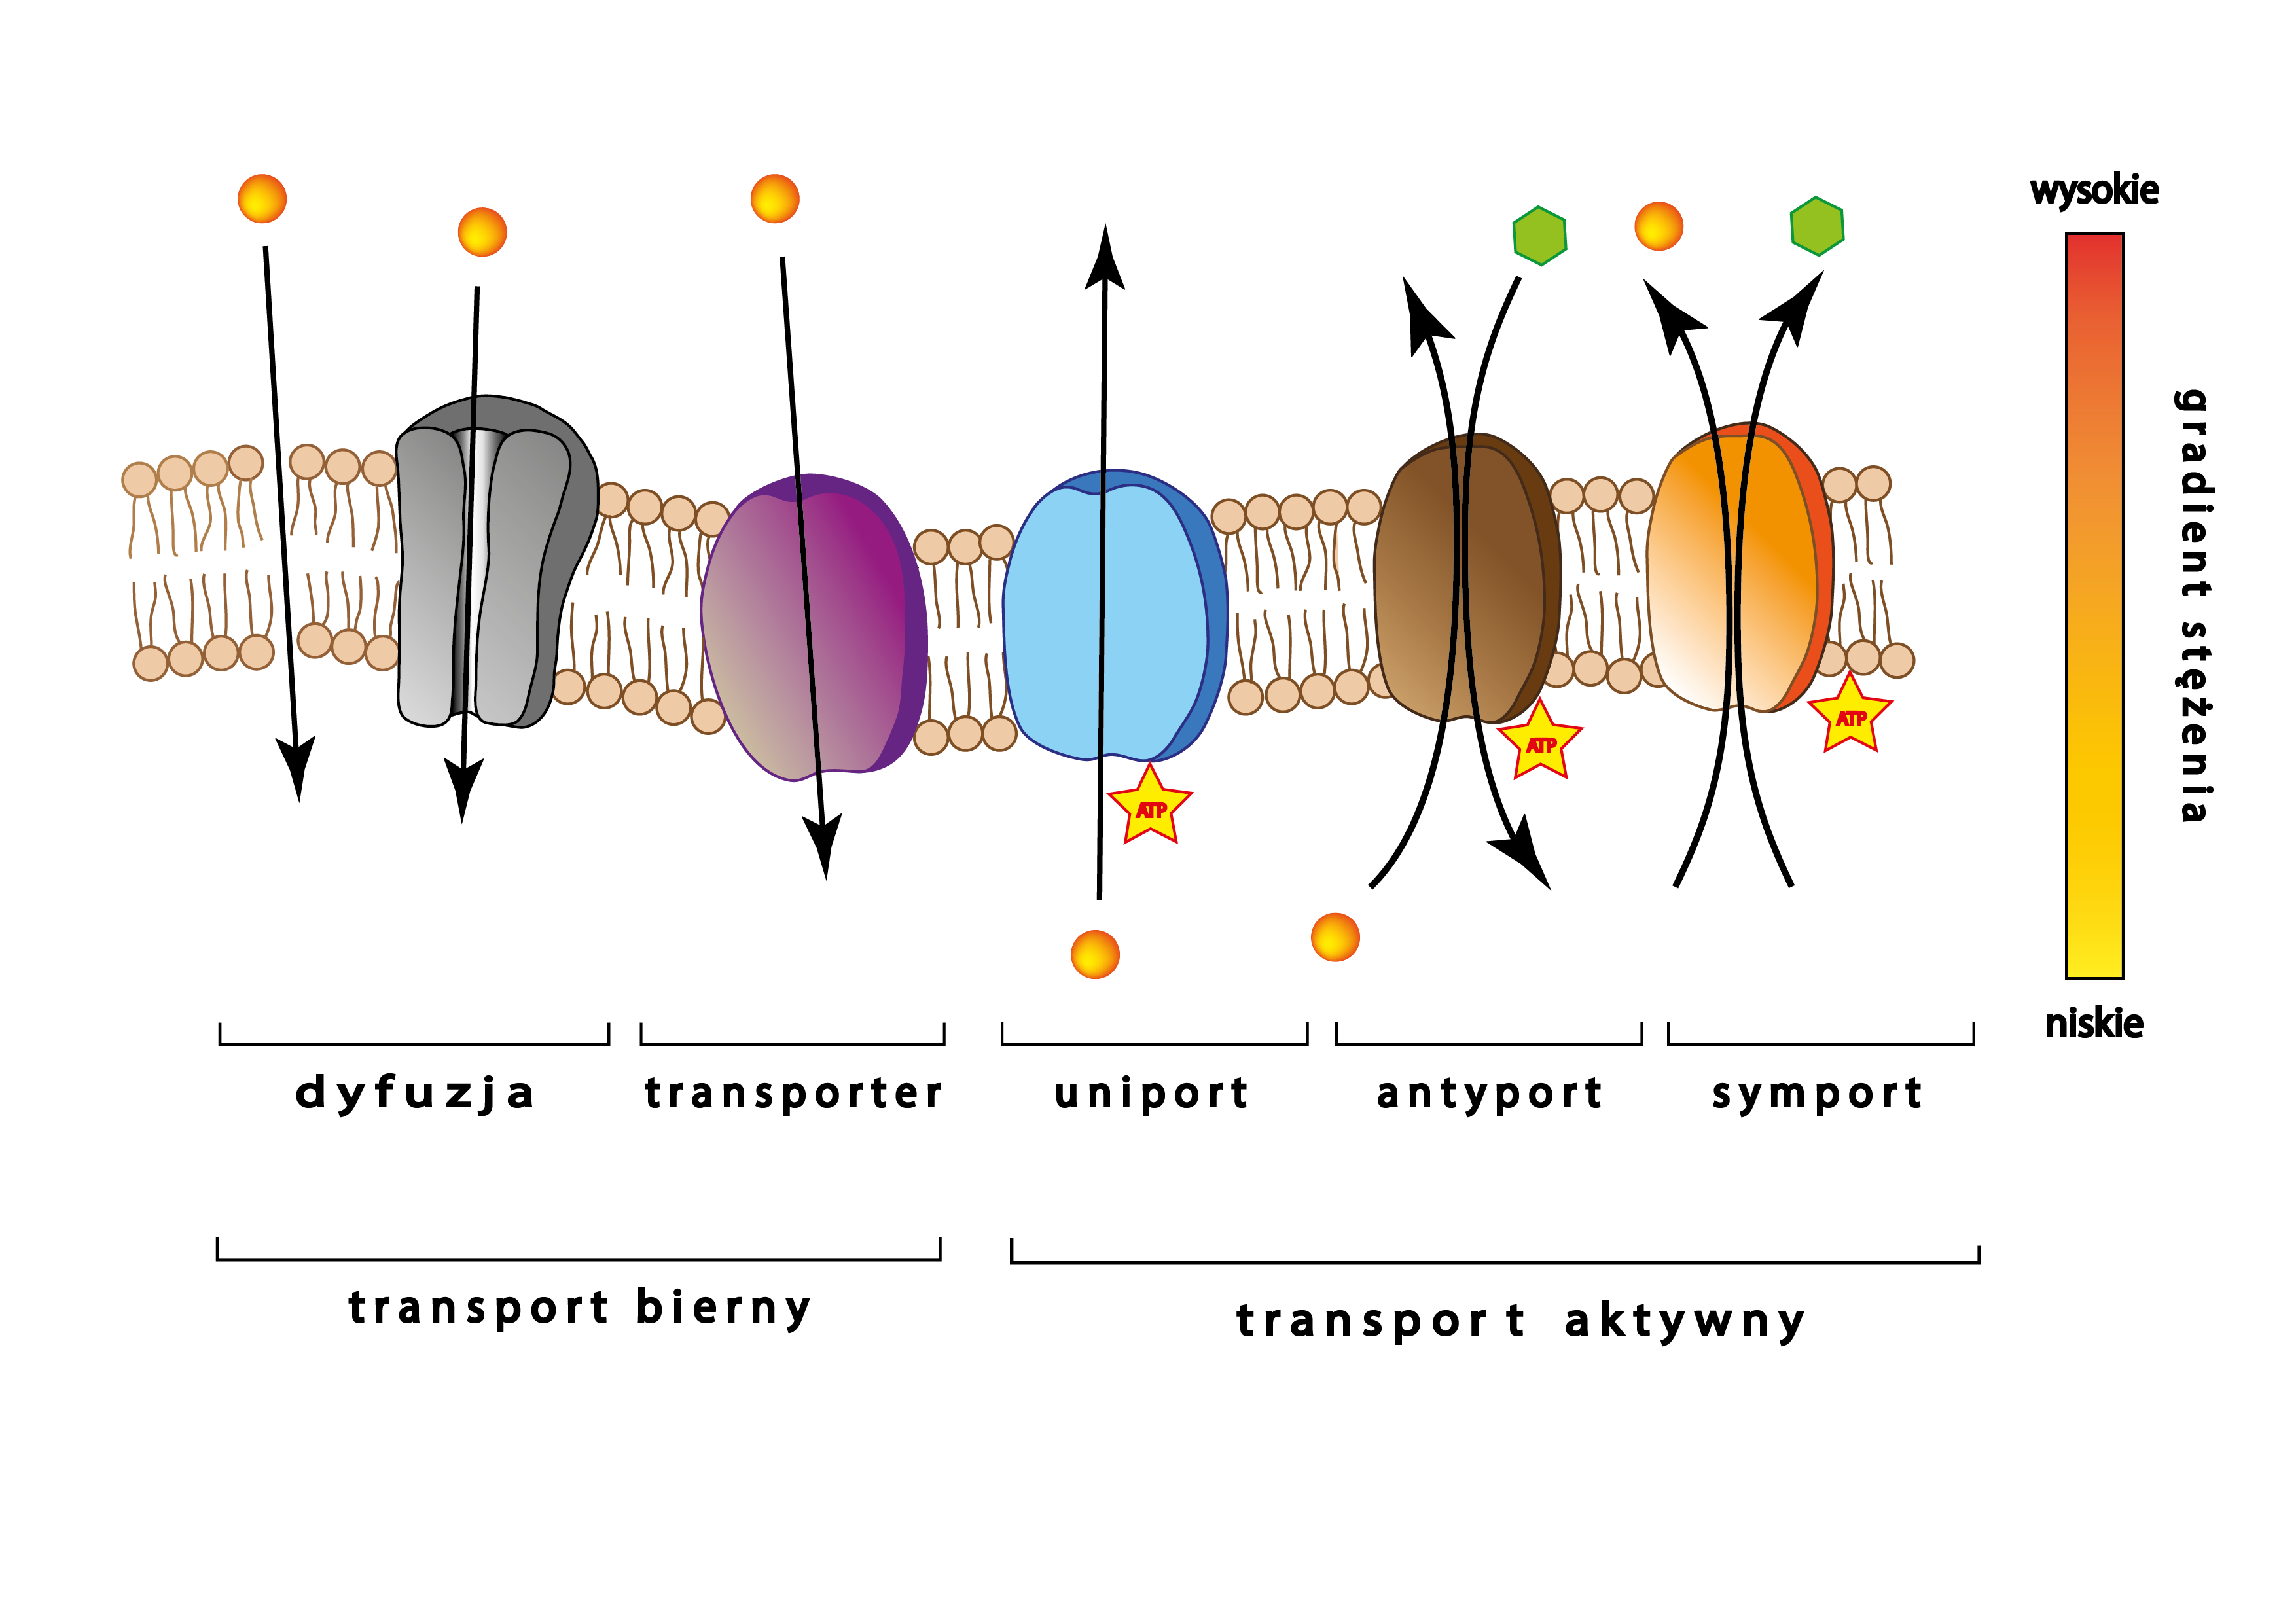
\includegraphics[width=0.85\textwidth]{rysunki/rozdzial_1/rodz_transportu.png}
\vspace{-40pt}
\caption{Różne rodzaje transportu w komórce.}
\label{fig:transport}
\end{figure}

Jeśli dwie substancje są przenoszone w tym samym kierunku, mówimy o \textbf{symporcie}, a jeśli w~przeciwnych kierunkach — o \textbf{antyporcie}. Jeżeli transport cząsteczki w~poprzek błony wymaga nakładu energii, mówimy o~transporcie aktywnym (czynnym). Transport czynny odbywa się w kierunku wyższego stężenia i~napięcia istniejącego w poprzek błony i~w~związku z tym białka realizujące ten rodzaj transportu często nazywane są ,,pompami'' - Ryc. \ref{fig:transport}. (W polskiej literaturze biologicznej termin ,,w kierunku wyższego stężenia'' zastępowany jest zwrotem ,,wbrew gradientowi stężeń''~\cite{Traczyk2007}.). Energia użyta do pracy pochodzi z rozkładu związków wysokoenergetycznych np. adenozyno-5'-trifosforanu (ATP)\nomenclature{ATP}{adenozyno-5'-trifosforan}. Białka przenoszące jedną substancję określa się jako uniporty lub \textbf{uniportery}. Szczególnymi przypadkami transportu aktywnego są kotransportery, które przenoszą jednocześnie dwie różne substancje (przez ten sam nośnik). Kotransportery wykorzystują różnicę gradientu jednej z transportowanych cząsteczek do przeniesienia innej. Gradient budowany jest z kolei przez inne białka przenoszące, tj. specyficzne pompy. Jeżeli substancje przenoszone są w tym samym kierunku mówimy o symporcie, natomiast w antyporcie każda z nich przenoszona jest w przeciwną stronę. Systemy antyportu nazywane są także mechanizmami wymiany. Wszystkie opisane powyżej mechanizmy wykorzystywane są do utrzymania homeostazy wapniowej w~komórce \cite{Traczyk2007}.

W procesach transportu jonów wapnia między komórką a otaczającym środowiskiem uczestniczą trzy systemy przenoszenia jonów:

\begin{bulletList}
\item kanały jonowe pracujące zgodnie z gradientem stężeń
\item aktywne pompy jonowe Ca$^{2+}$ ATP-aza i pompy protonowe (tzw. pierwszorzędowy system aktywnego transportu) przenoszące jony w kierunku wyższego stężenia jonów
\item układ kotransporterów (tzw. drugorzędowy system transportu wykorzystujący różnicę gradientów jonów sodowych i protonów wytworzoną przez aktywne pompy jonowe) działający ze znacznie mniejszą wydajnością.
\end{bulletList}


\section{Sygnałosom wapniowy}

Wapń jest jednym z 21 niezbędnych do życia pierwiastków. Całkowita ilość wapnia w organizmie człowieka wynosi około 1.5\% masy ciała. Jest składnikiem kości (jako hydroksyapatyt) i~stanowi istotny element wielu szlaków sygnalizacji wewnątrzkomórkowej \cite{Heaney2006}. Sygnalizacja wapniowa jest jedną z~najważniejszych w komórce. Kontroluje moment zapłodnienia oraz szereg procesów związanych z~różnicowaniem i~morfogenezą. Z kolei w dojrzałych komórkach sygnalizacja wapniowa ma wpływ na aktywność metaboliczną, sekrecję, ruch, przekaźnictwo sygnałów elektrycznych oraz plastyczność synaptyczną (p. rozdz.~\ref{sec:rolaCa}). Ostatecznie, podwyższona ilość wapnia w~komórce może doprowadzić do jej śmierci w~wyniku aktywacji szlaku programowanej śmierci (apoptozy - podrozdział~\ref{s:apoptoza}) lub bardziej chaotycznego procesu nekrotycznego (występującego podczas zawału lub niedotlenienia). Podstawowe grupy białek, które pełnią odrębne funkcje i~wchodzące w skład typowego sygnałosomu wapniowego to:\clearpage

\begin{bulletList}
\item białka transportujące wapń (kanały i pompy)
\item bufory wapniowe: białkowe (CaBP)\nomenclature{CaBP}{białka wiążące wapń \textit{ang. \textit{\textbf{ca}lcium \textbf{b}inding \textbf{p}roteins}}} i nieorganiczne \ce{PO4^3-}%(PO$_{4}^{3-}$)
\item sensory wapniowe (np. białka z rodziny kalmodulin)
\item białka efektorowe (kinazy białkowe)
\end{bulletList}

\newcommand{\ngray}{\rowcolor[gray]{.90}}
\begin{table}[h!]
\small
\centering
\begin{tabular}{lcccc} \toprule[0.12em]
 \textbf{Element}     & \textbf{Mięśnie}   & \textbf{Kardio-} & \textbf{Neurony}  & \textbf{Limfocyty} \\
 \textbf{Sygnałosomu}   & \textbf{Szkieletowe} & \textbf{miocyty} & \textbf{CA1}    &  \textbf{T}    \\\midrule[0.06em]
\textbf{Receptory}    &   --       & ET-1R/$\alpha$1R & mGluR1       & TCR        \\[0.3em]
             &           & AngIIR      & M1         &          \\[0.3em]
\textbf{PLC}       & --         & PLC$\beta$    & PLC$\beta$     & PLC$\gamma$1    \\[0.3em]
\textbf{EC}        & Ca$_V$1.1      & Ca$_V$1.2    & Ca$_V$1.2/Ca$_V$2.1& Orai1       \\[0.3em]
             &           &         & Ca$_V$2.2/NMDAR  &          \\[0.3em]
\textbf{RC}        & RyR1         & RyR2       & RyR2        & InsP$_3$R1     \\[0.3em]
             &           & InsP$_3$R2    & InsP$_3$R2     &          \\[0.3em]
\textbf{PMCA's}      & PMCA1a, 1c, 1d    & PMCA1c, 1d, 2a  & PMCA1a, 2a, 3a   & PMCA4b       \\[0.3em]
\textbf{SERCA's}     & SERCA1a, 1b     & SERCA2a     & SERCA2b, 3     & SERCA2b, 3     \\[0.3em]
\textbf{Wymienniki}    & NCX         & NCX1       & NCX1, 3      & --         \\[0.3em]
\textbf{Bufory}      & Parwalbumina     &   --      & Parwalbumina    &--         \\[0.3em]
             &           &         & Kalbindyna 28K   &          \\[0.3em]
\textbf{Sensory}     & Troponina C     & Troponina C   & Kalmodulina    & Kalmodulina    \\[0.3em]
             & Kalmodulina     & Kalmodulina   &          &          \\\bottomrule[0.12em]
\end{tabular}
\caption[Przykładowy sygnałosom]{Przykładowy układ elementów sygnałosomu wapniowego, specyficznego dla danego typu komórki. \textbf{EC} - kanały wpuszczające wapń do komórki; \textbf{RC} - kanały uwalniające wapń z~magazynów; \textbf{PMCA's} - pompy wapniowe na błonie komórkowej; \textbf{SERCA's} - pompy wapniowe siateczki sródplazmatycznej \cite{Berridge2012a}.}
\label{tab:sygnalosom}
\end{table}

Tak jak większość szlaków sygnalizacyjnych, szlak wapniowy rozpoczyna się w momencie aktywacji receptorów zewnątrzkomórkowych w postaci specyficznego bodźca chemicznego lub elektrycznego. Receptory przekazują informacje do różnego rodzaju przekaźników i wzmacniaczy (białko G, kinazy, fosfolipaza C), które wytwarzają substancje przekaźnikowe drugiego rzędu. Substancje te mają za zadanie przekazać sygnał z powierzchni komórki do rezydujących w cytozolu sensorów i efektorów. Substancje przekaźnikowe drugiego rzędu charakterystyczne dla wapniowej ścieżki sygnalizacyjnej to:

\begin{bulletList}
\item inozytolo 1,4,5-trifosforan (IP$_3$)\nomenclature{IP$_3$}{inozytolo 1,4,5-trifosforan} i diacyloglicerol (DAG) \nomenclature{DAG}{diacyloglicerol}, łączące aktywację receptora powiązanego z białkiem G z resztą wapniowej ścieżki sygnalizacyjnej i uwalnianie wapnia z magazynów wewnątrzkomórkowych
\item cykliczna ADP-ryboza (cADPR), uwalnia Ca$^{2+}$ z magazynów wewnątrzkomórkowych
\item fosforan dinukleotydu nikotynoamidoadeninowego (NADP)\nomenclature{NADP}{fosforan dinukleotydu nikotynoamidoadeninowego}
\item jony wapnia
\end{bulletList}

\textbf{Sensory} i \textbf{efektory}, podobnie jak \textbf{receptory} na powierzchni komórki, służą do detekcji przekaźników drugiego rzędu. Typowymi przykładami dla ścieżki wapniowej są białka wiążące wapń (np. kalmodulina), które wykrywają zwiększenie stężenia wapnia w cytozolu i przekazują tę informację do różnych efektorów kontrolujących takie procesy jak skurcz włókienek aktynowo-miozynowych, czy sekrecja. Niekiedy sensory są równocześnie efektorami, np. enzymy wrażliwe na cykliczne nukleotydy (np. cAMP/cGMP). Efektory mogą tworzyć również skomplikowany system złożony z wielu komponentów, np. system sterujący procesami egzocytozy, fagocytozy, czy transkrypcji genów, odpowiedzialne za aktywację specyficznej odpowiedzi komórkowej.

Różnorodność sygnalizacji wapniowej osiągana jest za pomocą dużej ilości białek efektorowych wrażliwych na wapń. Wszystkie białka zaangażowane w przekazywanie sygnału wapniowego tworzą tzw. ,,\textbf{sygnałosom wapniowy}''. Poszczególne rodzaje komórek zawierają różne elementy sygnałosomu, który dostosowany jest do typu komórki i~funkcji, jakie pełni (Tab.~\ref{tab:sygnalosom}). W taki sposób każda komórka generuje specyficzny sobie sygnał wapniowy. Istotną właściwością każdego sygnałosomu jest fakt, iż wraz rozwojem i różnicowaniem komórek ulega on przebudowie, co może wpłynąć na charakter odpowiedzi komórkowej na sygnał wapniowy.

Podstawowymi elementami białkowymi biorącymi udział w transdukcji sygnału wapniowego są \cite{Berridge2012,Lytton2007,Schwaller2012}:

\begin{bulletList}
\label{bialkaTransportowe}

\item kanały wapniowe (transport bierny):
	\begin{itemize}[label=\textopenbullet]
	\item kanały wapniowe błony komórkowej (bramkowane napięciem -VGCC)\nomenclature{VGCC}{kanały wapniowe bramkowane napięciem (ang. \textit{\textbf{v}oltage \textbf{g}ated \textbf{c}alcium \textbf{c}hannels})} \\ i~bramkowane ligandem - (LGCC)\nomenclature{LGCC}{kanały wapniowe bramkowane ligandem (ang. \textit{\textbf{l}igand \textbf{g}ated \textbf{c}alcium \textbf{c}hannels})}
	\item kanały transportujące wapń z siateczki śródplazmatycznej: receptor\\ \mbox{inozytolo-3-fosforanu} (IP$_3$R) \nomenclature{IP$_3$R}{receptor inozytolo-1,4,5-trifosforanu} oraz receptor rianodynowy (RyR)\nomenclature{RyR}{receptor rianodynowy}
	\item kanały transportujące wapń do mitochondrium - VDAC \nomenclature{VDAC}{ang. \textit{\textbf{v}oltage \textbf{d}ependent \textbf{a}nion \textbf{c}hannel}} oraz mitochondrialny uniporter
	\item kanały pojemnościowego napływu jonów wapniowych (SOCEC)\nomenclature{SOCEC}{kanały pojemnościowego napływu jonów wapniowych (ang. \textit{\textbf{s}tore-\textbf{o}perated \textbf{c}alcium \textbf{e}ntry \textbf{c}hannels})}
	\item kanały wapniowe aktywowane poprzez receptor (ROCC)\nomenclature{ROCC}{kanały wapniowe aktywowane poprzez receptor (ang. \textit{\textbf{r}eceptor \textbf{o}perated \textbf{c}alcium \textbf{c}hannels})}
	\item kanały TRPC (ang. transient receptor potential channel)\nomenclature{TRPC}{ang. \textit{\textbf{t}ransient \textbf{r}eceptor \textbf{p}otential \textbf{c}hannel}}
	\end{itemize}
\item pompy wapniowe (transport czynny)
	\begin{itemize}[label=\textopenbullet]
	\item plazmatyczna Ca$^{2+}$-ATPaza (PMCA)\nomenclature{PMCA}{plazmatyczna Ca$^{2+}$-ATPaza (ang. \textit{\textbf{p}lasma \textbf{m}embrane \textbf{c}alcium \textbf{A}TPaze})}
	\item sarko(endo)plazmatyczna Ca$^{2+}$-ATPaza (SERCA)\nomenclature{SERCA}{sarko(endo)plazmatyczna Ca$^{2+}$-ATPaza (ang. \textit{\textbf{s}arco(\textbf{e}ndo)-\textbf{p}lasmatic \textbf{c}alcium \textbf{A}TPaze})}
	\end{itemize}
\item wymienniki wapniowe (transport czynny)
	\begin{itemize}[label=\textopenbullet]
	\item wymiennik sodowo/wapniowy (NCX)\nomenclature{NCX}{wymiennik sodowo/wapniowy (ang. \textit{\textbf{N}a/\textbf{C}a e\textbf{x}changer})}
	\item wymiennik sodowo/wapniowo/potasowy (NKCX)\nomenclature{NKCX}{wymiennik sodowo/wapniowo/potasowy (ang. \textit{\textbf{N}a/\textbf{K}/\textbf{C}a e\textbf{x}changer})}
	\end{itemize}
\end{bulletList}

%Praca ta zawiera analizę modelu przepływu jonów wapnia w komórce, ze szczególnym uwzględnieniem specyficznych struktur, tworzących się na styku kompartmentów sub-komórkowych: siateczki śródplazmatycznej i mitochondriami.


\section{Rola jonów wapnia w komórce}
\label{sec:rolaCa}

\begin{wrapfigure}{o}{0.6\textwidth}
%\vspace{-10pt}
  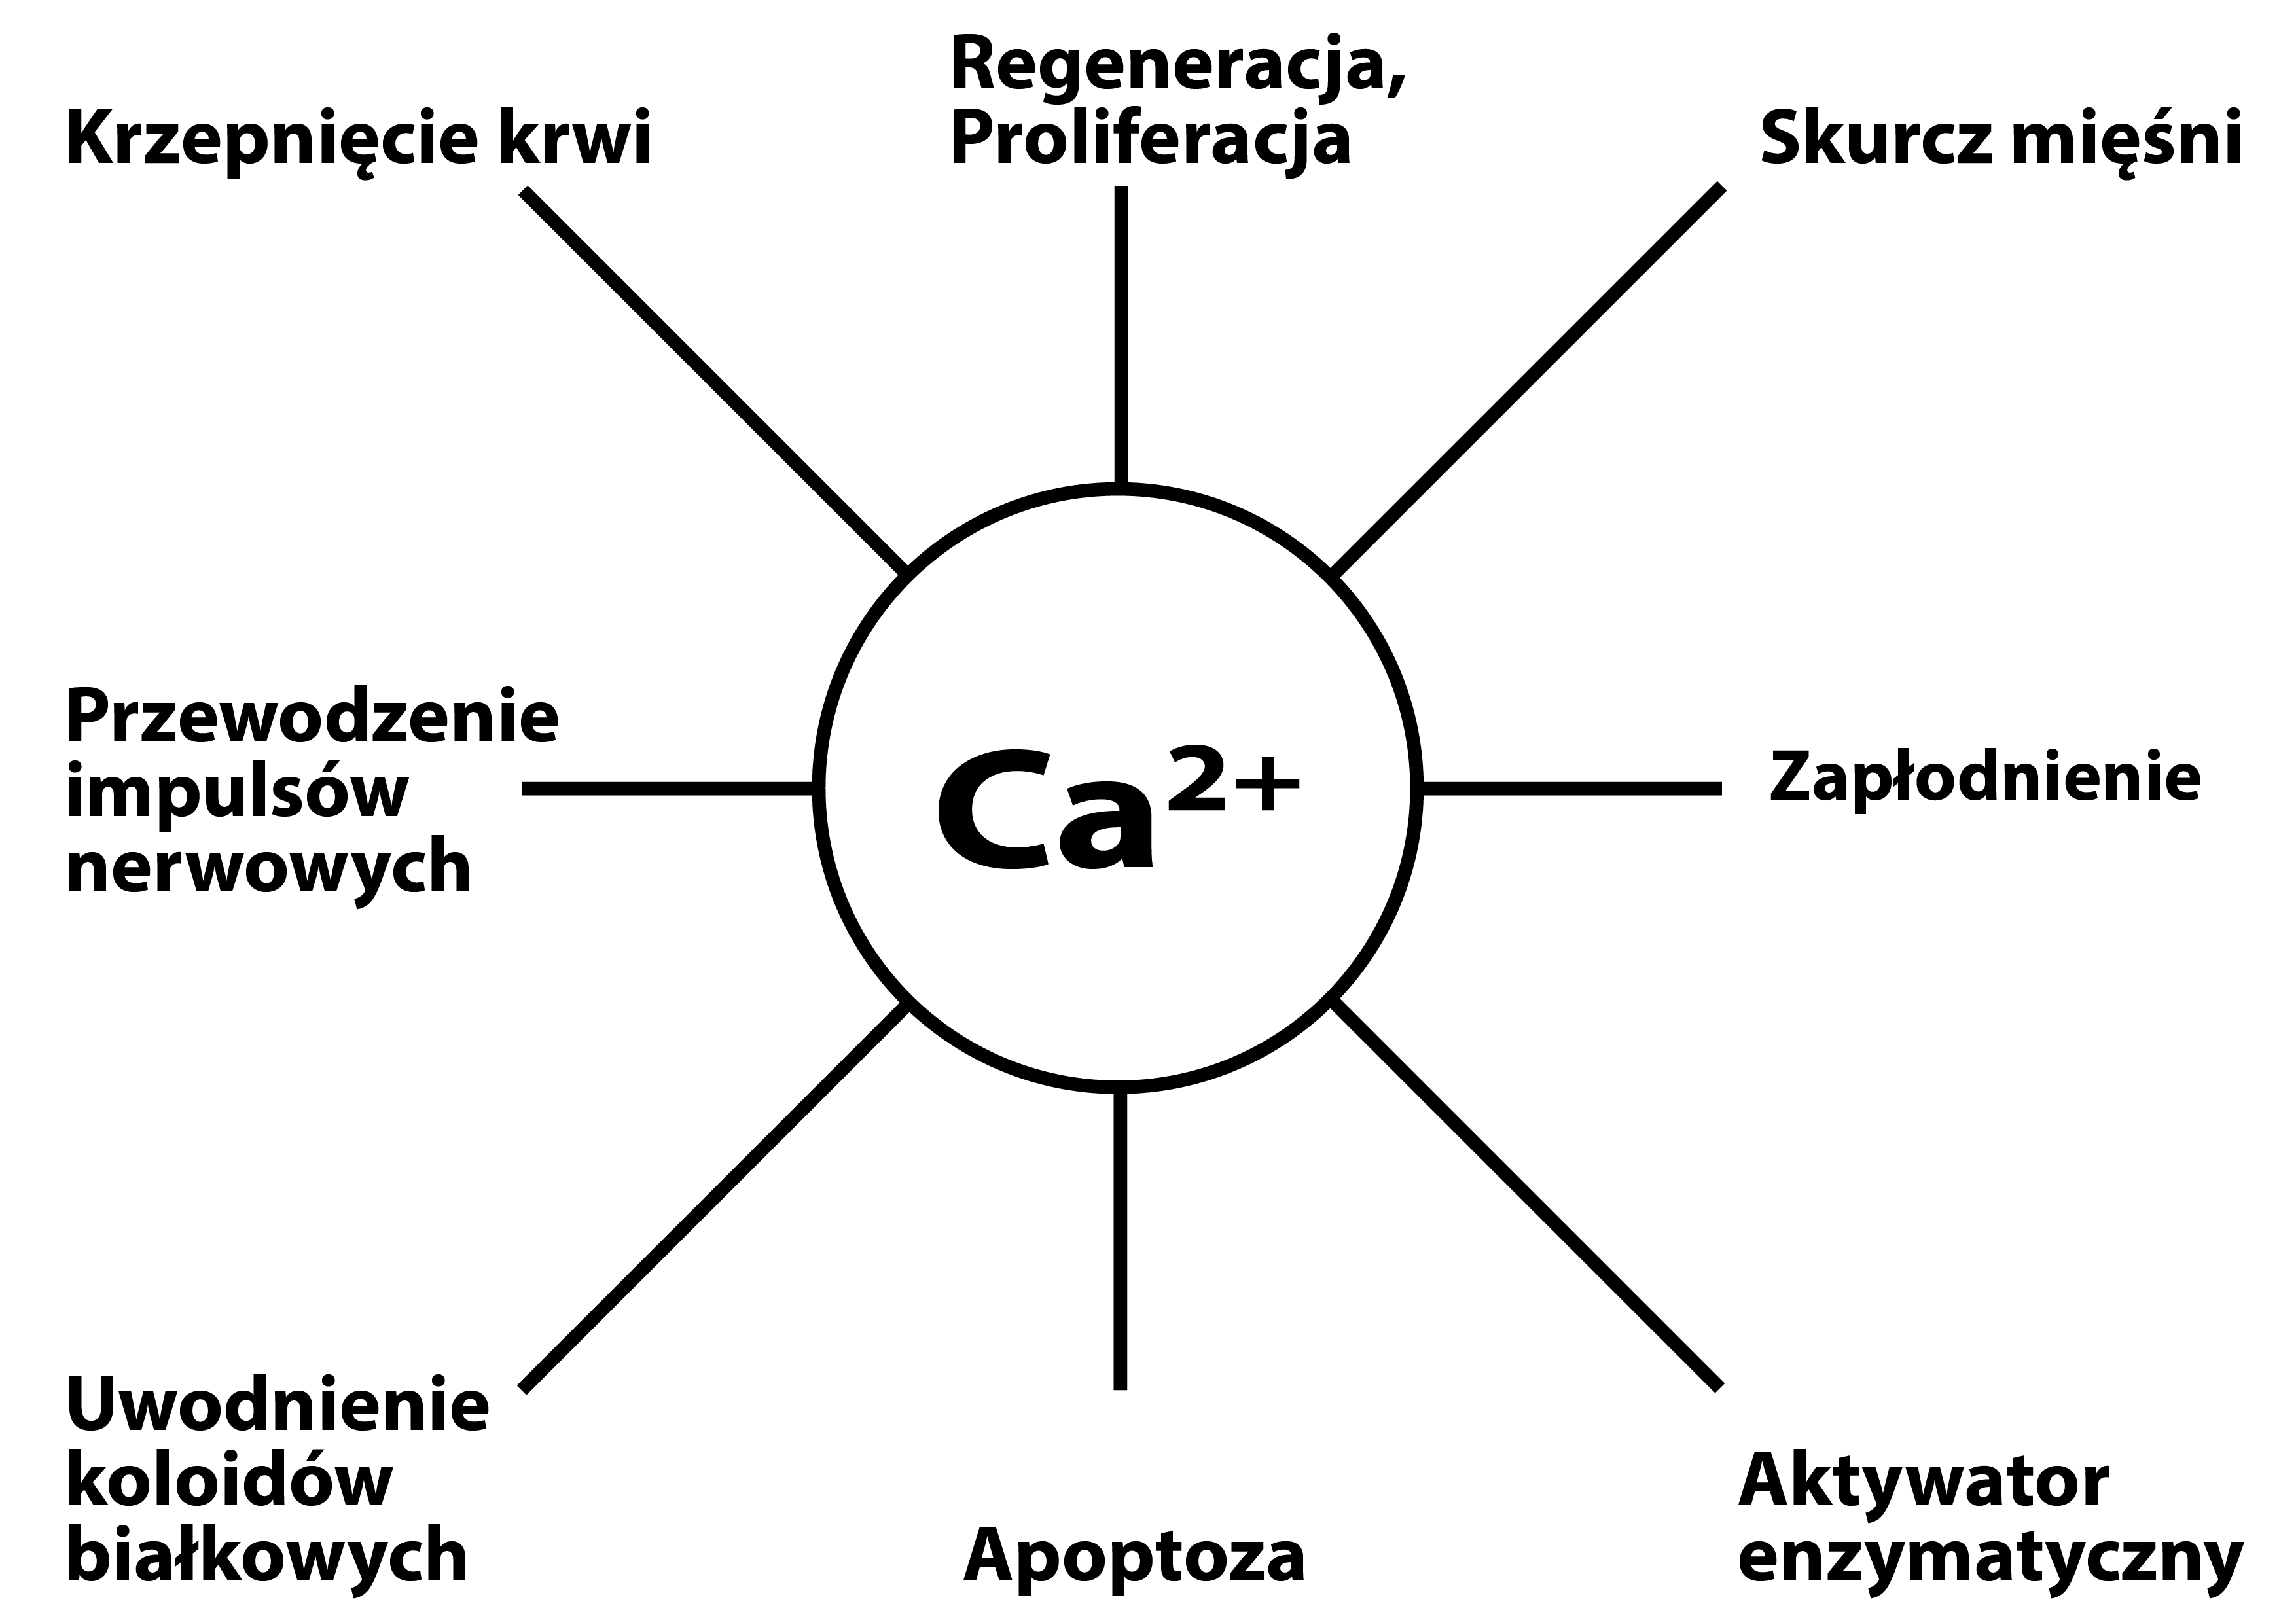
\includegraphics[width=0.58\textwidth]{rysunki/rozdzial_1/funkcjeCa.png}
 \caption[Udział jonów Ca$^{2+}$ w integracji szlaków sygnałowych]{Udział jonów wapnia w integracji różnych szlaków i procesów komórkowych.}
 \label{fig:integracja}
\end{wrapfigure}

W toku ewolucji wytworzyło się wiele mechanizmów wykorzystujących wapń jako cząsteczkę sygnałową do realizacji specyficznych procesów fizjologicznych działających w różnych ramach czasowych. Sygnał wapniowy może działać od kilkunastu mikrosekund, po wiele godzin. Szybkie zmiany związane bezpośrednio z wahaniami stężenia wapnia w cytozolu obejmują takie zjawiska jak: skurcz mięśni poprzecznie prążkowanych, sekrecja hormonów, wzmożona produkcja ATP. Zmiany te zachodzą w komórce w ciągu sekund lub kilku minut. W dłuższej perspektywie czasu aktywowane są różne mechanizmy kontrolujące ekspresje genów w komórce, które mogą wpływać na różnicowanie komórek, proliferację, cykl komórkowy lub programowaną śmierć. Tego typu reorganizacja czynności komórki wymaga dłuższego czasu i zajmuje od kilku do kilkunastu godzin.

Wapń w cytozolu stanowi więc przekaźnik informacji i może być używany jako sygnał integrujący procesy zachodzące w różnych przedziałach komórki lub sygnał przekazujący informację pomiędzy środowiskiem zewnętrznym, a komórką lub pomiędzy komórkami. Stanowi kluczowy element integrujący szereg szlaków sygnalizacyjnych i~procesów: mechano-chemicznych, biochemicznych i elektrycznych (Ryc.~\ref{fig:integracja}). Aktywowane szlaki sygnalizacyjne prowadzą do zmian w~funkcjonowaniu komórki, które mogą objawiać się w bardzo różnorodny sposób - od apoptozy po skurcz mięśni i kontrolę procesu zapłodnienia.

\subsection{Sprzężenie mechano-chemiczne (skurcz mięśni)}

Wszystkie typy mięśni wykazują zdolność do odpowiadania skurczem na docierające do nich sygnały elektryczne/chemiczne. Elementami kurczliwymi są włókienka fibrylarne tworzące sarkomer. Skrócenie sarkomeru wymaga energii dostarczanej przez hydrolizę związku wysokoenergetycznego ATP do ADP\nomenclature{ADP}{adenozyno-5'-difosforan} i reszty fosforanowej. W obu typach mięśni (gładkich i poprzecznie prążkowanych) czynnikiem inicjującym skurcz jest wzrost stężenia jonów wapnia w cytoplazmie. Ciąg zdarzeń następujący od momentu inicjacji sygnału elektrycznego do skurczu mięśnia nosi nazwę sprzężenia mechano-chemicznego.


\paragraph{Etap 1}
Potencjał czynnościowy osiąga akson neuronu ruchowego. Potencjał czynnościowy aktywuje kanały wapniowe zależne od napięcia zlokalizowane w błonie komórkowej aksonu, co powoduje gwałtowne wnikanie jonów wapnia Ca$^{2+}$ do wnętrza komórki. Pod wpływem kaskady sygnałowej uruchomionej zwiększonym stężeniem wapnia, pęcherzyki zawierające acetylocholinę łączą się z~błoną komórkową uwalniając neurotransmiter do szczeliny płytki nerwowo-mięśniowej.



\noindent Acetylocholina dyfunduje przez szczelinę, łącząc się na jej drugim końcu z receptorami nikotynowymi, co powoduje otwarcie kanałów sodowych i potasowych zlokalizowanych w błonie komórkowej miocytu. Przewaga jonów sodu powoduje depolaryzację błony komórkowej i powstanie dodatniego potencjału czynnościowego. Pod wpływem potencjału czynnościowego retikulum endoplazmatyczne komórki mięśniowej uwalnia jony wapnia.

\paragraph{Etap 2}
Mechanizm skurczu opisuje ,,ślizgowa teoria skurczu''. Skracanie białek fibrylarnych jest wynikiem oddziaływań pomiędzy włóknami aktyny i~miozyny, powiązanych z troponiną C (tzw. tropomiozyna). Zwiększenie stężenia jonów wapnia w cytozolu powoduje zmianę konformacji troponiny C. Kompleks tropomiozyny zmienia swoje położenie względem aktyny, odsłaniając miejsca kontaktu znajdujące się na włóknie aktynowym. Umożliwia to oddziaływanie aktyny z miozyną. Główki miozyny po połączeniu z~aktyną, pod wpływem ADP przesuwają się, doprowadzając do przemieszczenia się włókienek względem siebie, co w efekcie powoduje wsuwanie się filamentów aktynowych głębiej pomiędzy filamenty miozynowe co prowadzi do skracania się sarkomeru. Główki miozyny pod wpływem ATP odłączają się od aktyny. Etap ten powtarzany jest przez cały czas, kiedy w cytozolu utrzymuje się podwyższone stężenie jonów wapnia.

W mięśniach gładkich nie ma troponiny C. Procesem inicjującym skurcz jest w nich fosforylacja lekkiego łańcucha miozyny przez zależną od kalmoduliny i wapnia kinazę lekkich łańcuchów miozyny.

\paragraph{Etap 3}
Wapń jest aktywnie wpompowywany z powrotem do zbiorników retikulum endoplazmatycznego przez pompę wapniową (Ca/ATP-azę). Tropomiozyna wraca do pierwotnej konfiguracji, blokując miejsca wiązania miozyny na aktynie.

\bigskip
\FloatBarrier
\subsection{Regulacja procesów biochemicznych}\label{ss:metabo}

W wyniku związania ligandu lub zmiany różnicy napięć na powierzchni błony komórkowej, do komórki dostają się jony wapnia. Jony te są w stanie regulować aktywność szeregu protein, które w tym kontekście nazywane są białkami efektorowymi. Białka takie posiadają zdolność regulacji aktywności innych białek, należących do kaskady sygnałowej. Jednym z pierwszych poznanych białek efektorowych zależnych od wapnia była kalmodulina. Przyłączenie czterech jonów wapnia powoduje zmianę konformacji kalmoduliny, w~wyniku czego może ona oddziaływać z innymi białkami. W~ten sposób aktywowanych jest wiele enzymów zależnych od kalmoduliny (m.in. kinaza II). Kinazy aktywują inne białka, charakterystyczne dla danej kinazy, co w efekcie prowadzi do propagacji sygnału, który może dawać różnorodne efekty zależne od obecności w komórce poszczególnych elementów sygnałosomu. W odpowiedzi na aktywację kalmoduliny w~komórce mogą zostać aktywowane szlaki odpowiedzialne za takie procesy jak: procesy zapalne, apoptozę, ekspresję genów, transport wewnątrzkomórkowy lub regulację cyklu komórkowego \cite{Berridge2012i}.

Sygnalizacja wapniowa oparta na receptorach metabotropowych polega na stymulacji receptorów błonowych sprzężonych z białkami G, które aktywują \textbf{fosfolipazę C} (PLC)\nomenclature{PLC}{fosfolipaza C}. Enzym ten powoduje hydrolizę 4,5-difosforanu fosfatydyloinozytolu do inozytolotrifosforanu (IP$_3$), który wiąże się z receptorami \textbf{IP$_3$R} oraz \textbf{diacyloglicerolu} (DAG). Po związaniu IP$_3$ prowadzi do uwolnienia jonów wapnia z siateczki śródplazmatycznej do cytoplazmy. Sygnał wapniowy następnie może być propagowany w postaci fali wapniowej lub aktywować szereg kinaz białkowych zależnych od wapnia (Ryc.~\ref{fig:transdukcja}). DAG z kolei jest przekaźnikiem drugiego rzędu, który docelowo aktywuje rodzinę kinaz białkowych typu C (PKC)\nomenclature{PKC}{kinaza białkowa typu C}. PKC reguluje aktywność kilkudziesięciu innych białek \cite{Newton1995}.

W zależności od organellum i właściwości sygnału wapniowego, aktywowane mogą być różne ścieżki efektorowe. W~mitochondrium, wapń w ilościach mikromolowych, stymuluje produkcję ATP poprzez regulację allosteryczną trzech dehydrogenaz cyklu Krebsa: pirogronianowej, izocytrynianowej oraz $\alpha$-ketoglutaranowej \cite{Denton2009,Griffiths2009}. W~momencie, kiedy poziom wapnia utrzymuje się na podwyższonym poziomie przez dłuższy czas, mitochondria akumulują znaczne ilości tego jonu, co może doprowadzić do precypitacji fosforanu wapnia, produkcji reaktywnych form tlenu i utraty mitochondrialnego potencjału transbłonowego. Skutkuje to zwiększeniem ich objętości, powstają wtedy specyficzne pory permeabilizacyjne PTP (ang. \textit{\textbf{p}ermeability \textbf{t}ransition \textbf{p}ore})\nomenclature{PTP}{ang. \textit{\textbf{p}ermeability \textbf{t}ransition \textbf{p}ore}}, które uwalniają zawartość matriks do cytozolu. Pośród uwolnionych czynników znajdują się m. in.czynnik indukujący apoptozę (AIF ang. \textit{\textbf{a}poptosis \textbf{i}nducing \textbf{f}actor})\nomenclature{AIF}{ang. \textit{\textbf{a}poptosis \textbf{i}nducing \textbf{f}actor}} i cytochrom C, odpowiedzialne za aktywację kaspaz (ang. \textit{caspases -- \textbf{c}ysteine-dependent \textbf{asp}artate specific protea\textbf{ses}}) i wejście komórki na szlak apoptotyczny (Ryc.~\ref{fig:apoptoza}) \cite{Demaurex2003,Desagher2000}.

W jądrze komórkowym, które otoczone jest podwójną błoną białkowo-lipidową, tzw. otoczką jądrową (jej przedłużenie stanowi szorstka siateczka śródplazmatyczna, określana jako RER (ang. \textbf{r}ough \textbf{e}ndoplazmic \textbf{r}eticulum))\nomenclature{RER}{szorstka siateczka śródplazmatyczna (ang. \textbf{r}ough \textbf{e}ndoplazmic \textbf{r}eticulum)}, wzrost stężenia Ca$^{2+}$ może wpłynąć na transkrypcję genów pośrednio lub bezpośrednio. Pośrednio - poprzez aktywację jądrowych kinaz zależnych od wapnia, albo bezpośrednio, w~wyniku aktywacji czynników transkrypcyjnych wiążących Ca$^{2+}$ \cite{Gomes2006}. Jądro komórkowe określane jest czasami jako komórka wewnątrz komórki, ponieważ otoczka jądrowa zawiera własne elementy metabotropowej gałęzi szlaku sygnalizacji wapniowej, takie jak PLC, PKC, IP$_3$R, RyR, które generują osobne impulsy wapniowe wewnątrz jądra \cite{Rodrigues2009}.


W oocytach fala wapniowa uwolniona w momencie wniknięcia plemnika powoduje zmianę organizacji osłon jaja. Mechanizm polega na aktywacji i dyfuzji specyficznej dla plemników fosfolipazy C uwalnianej w~wyniku fuzji plemnika i oocytu. Gwałtowna zmiana stężenia wapnia propaguje się w postaci fali wapniowej rozchodzącej się po obwodzie całej komórki i doprowadza do zlewania się drobnych pęcherzyków z przestrzeni podbłonowej z błoną komórkową. Zawartość pęcherzyków modyfikuje skład otoczki oocytu \cite{Whitaker2006}.

\begin{figure}[tb]
\centering
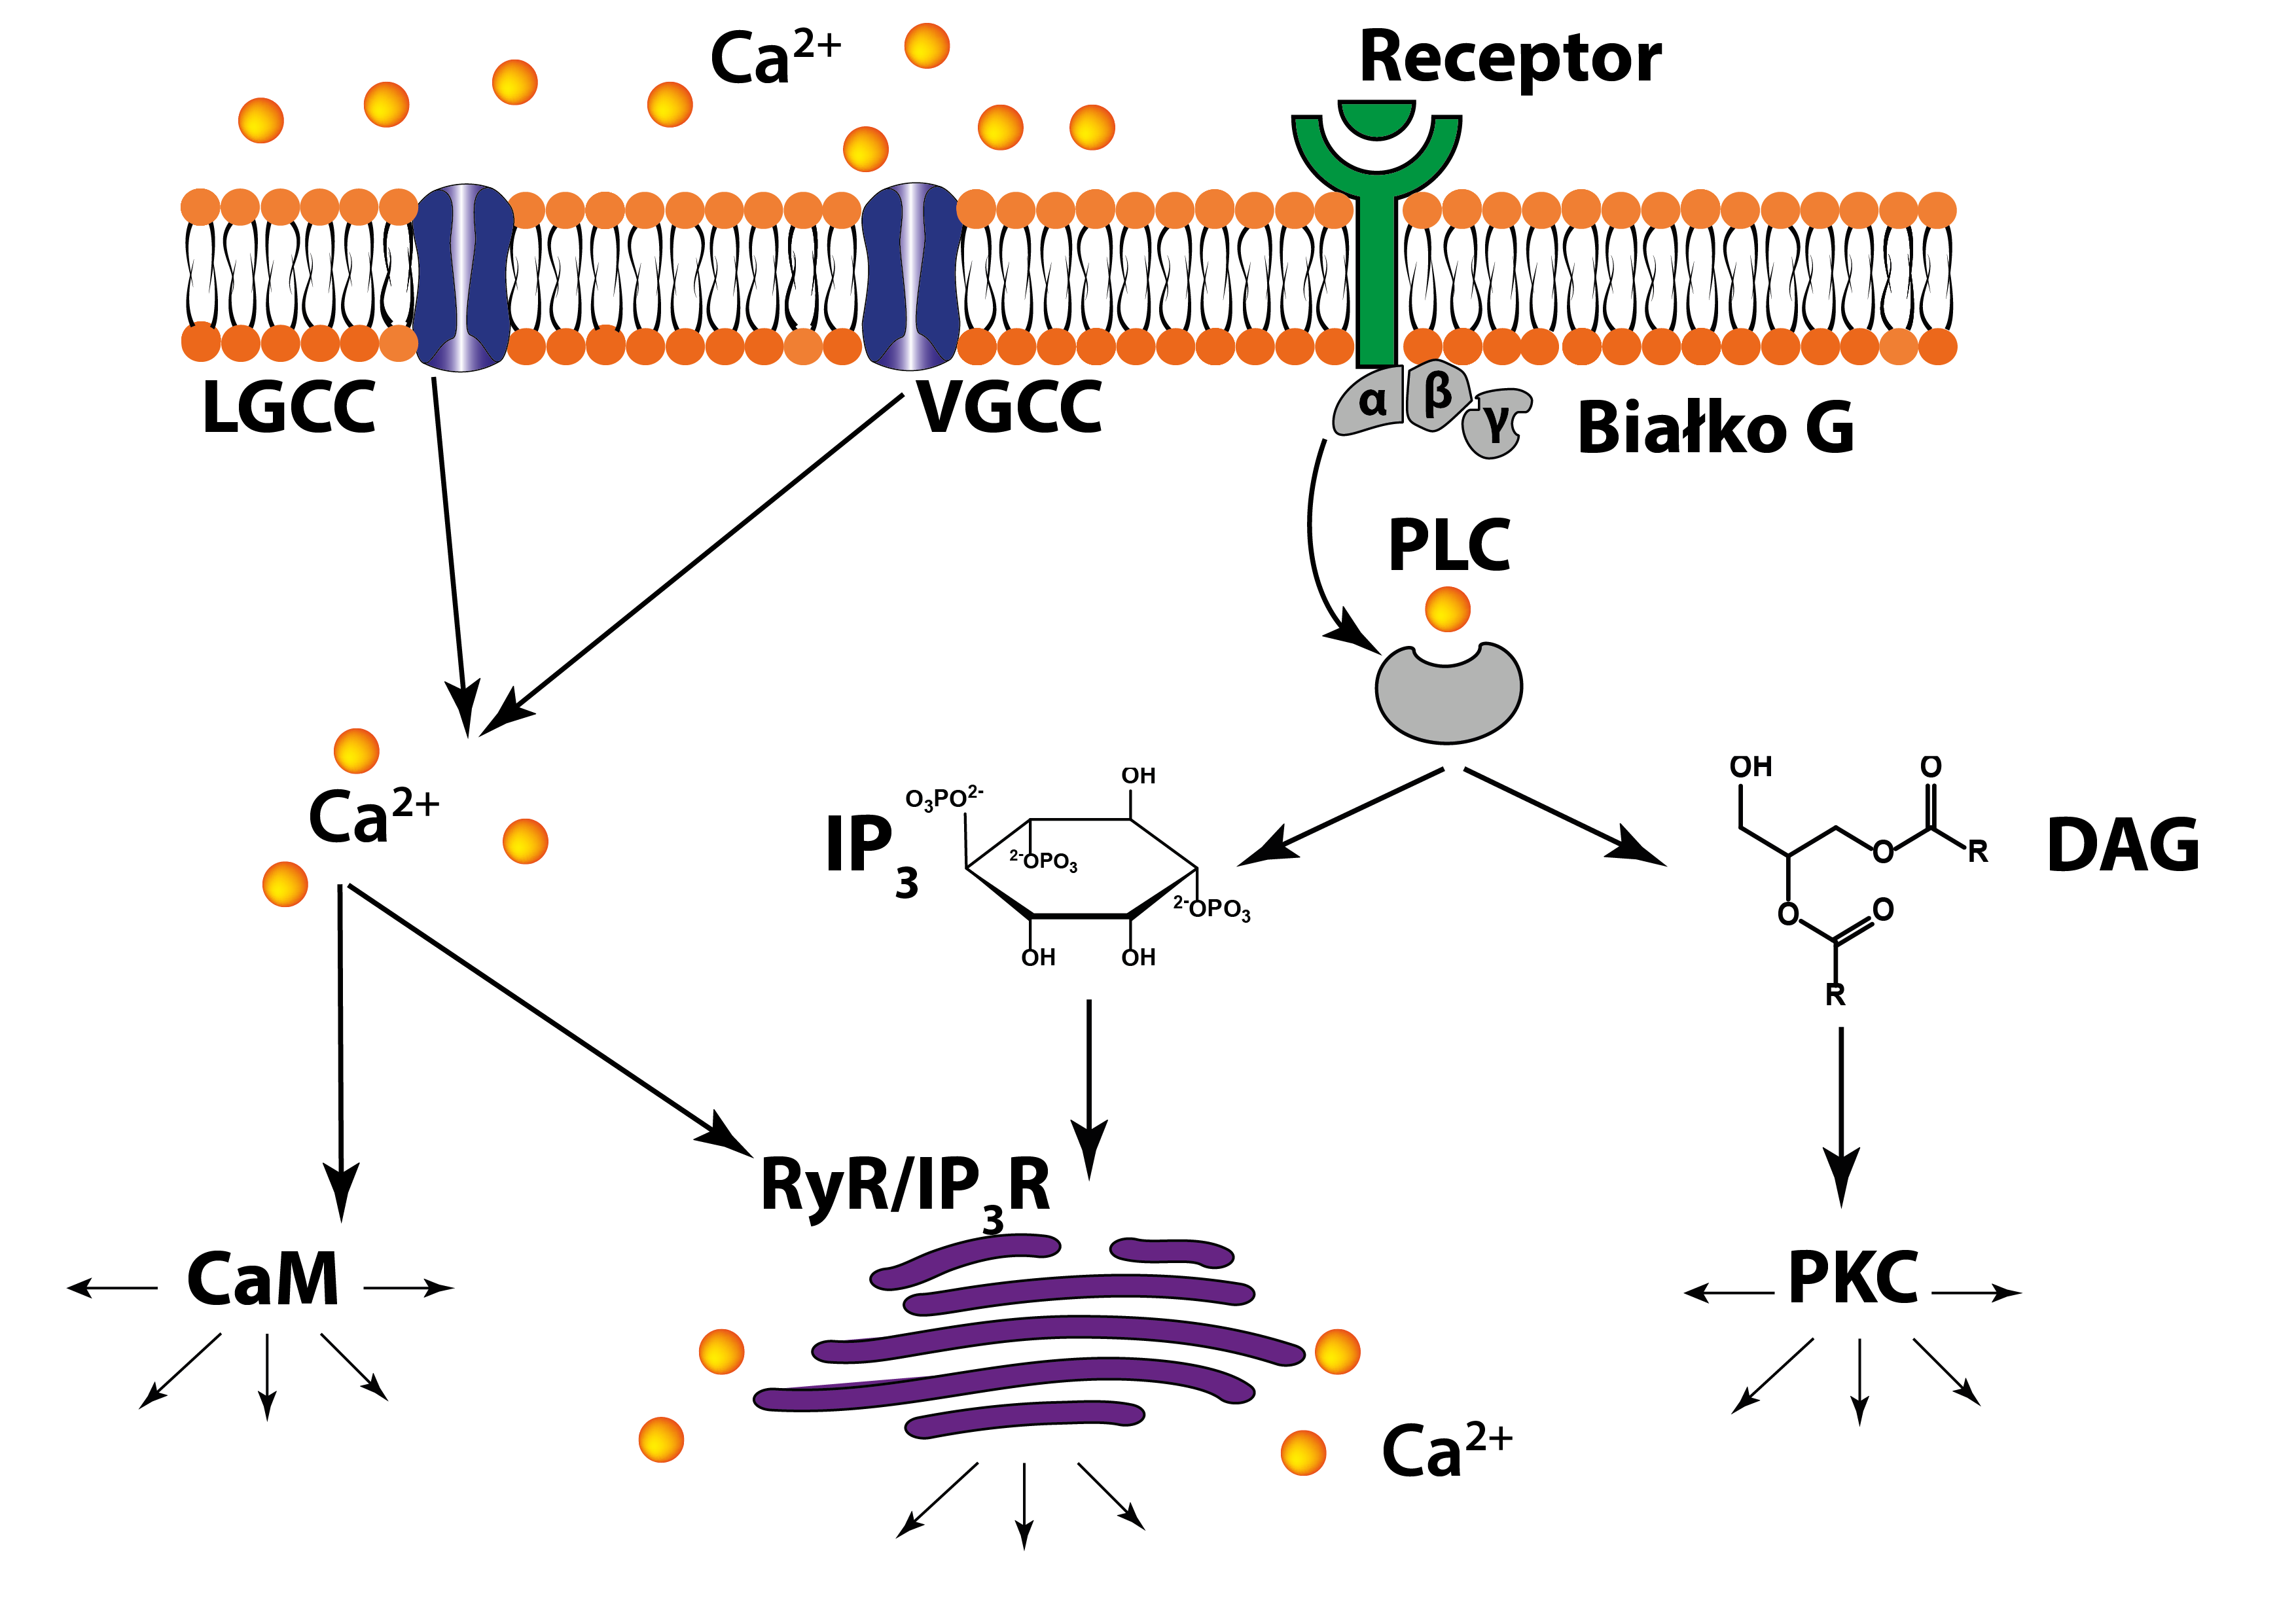
\includegraphics[width=0.99\textwidth]{rysunki/rozdzial_1/transdukcja.png}
\caption[Transdukcja sygnału wapniowego]{Transdukcja sygnału wapniowego w komórce: kanały wapniowe bramkowane napięciem (\textbf{VGCC}) i ligandem (\textbf{LGCC}); \textbf{PLC}: fosfolipaza typu C; \textbf{CaM}: kalmodulina; \textbf{IP$_3$}: inozytolo-1,4,5-trifosforan; \textbf{DAG}: diacyloglicerol; \textbf{IP$_3$R} receptor inozytolo-1,4,5-trifosforanu; \textbf{PKC}: kinaza białkowa typu C.}
\label{fig:transdukcja}
\end{figure}

\subsection{Regulacja sygnałów elektrycznych}
Sygnalizacja elektryczna odgrywa znaczącą rolę w komunikacji komórek pobudliwych np. syncytia serca, neurony, tkanka glejowa. W neuronach niektóre receptory neuroprzekaźników (NMDAR, AMPAR, 5-HTR) sprzężone są z kanałami wapniowymi (kanały bramkowane ligandem - LGCC, Rozdz.~\ref{ss:lgcc}), obecnymi w błonach komórek pobudliwych. Obecne są też kanały wapniowe bramkowane napięciem (VGCC, Rozdz.\ref{ss:vgcc}). Aktywacja tych kanałów prowadzi do napływu Ca$^{2+}$ do wnętrza komórki, co zmniejsza różnicę potencjału elektrycznego utrzymywanego w poprzek błony komórkowej (tzw. potencjał spoczynkowy równy -70 mV). Po osiągnięciu wartości progowej (-50 mV) następuje otwarcie bramkowanych napięciem kanałów przewodzących odkomórkowo jony potasowe, oraz kanałów przewodzących jony sodowe do wnętrza komórki. Aktywowane są również kanały przepuszczające jony chlorkowe na zewnątrz komórki. Otwarcie tych kanałów powoduje ruch jonów zgodny z gradientami ich stężeń, który szybko niweluje różnicę potencjałów pomiędzy środowiskiem zewnątrz- i wewnątrzkomórkowym i~wskutek szybkiego napływu sodu rośnie do wartości +35 mV. Jest to tzw. potencjał czynnościowy. Skutkiem ucieczki chloru jest narastająca depolaryzacja błony komórkowej spowalniana i osłabiana przez hiperpolaryzujące działanie wypływających z komórki jonów potasu \cite{Bear2007,Traczyk2007}.

W mięśniach rezultatem depolaryzacji jest otwarcie zależnych od napięcia kanałów wapniowych (kanały typu L) i dalszy wzrost stężenia jonów wapnia w cytozolu. Sygnał wapniowy prowadzi do aktywacji kanałów rianodynowych, znajdujących się na powierzchni siateczki śródplazmatycznej. Generuje to kolejną falę wapniową spowodowaną wyrzutem wapnia z magazynu komórkowego. Mechanizm ten nosi nazwę \textbf{CICR} (ang. \textit{\textit{\textbf{c}alcium \textbf{i}nduced \textbf{c}alcium \textbf{r}elease}})\nomenclature{CICR}{wypływ wapnia aktywowany wapniem (ang. \textit{\textbf{c}alcium \textbf{i}nduced \textbf{c}alcium \textbf{r}elease}}. W~komórkach nerwowych prowadzi to do uwolnienia neurotransmiterów w synapsach. Stanowi też podstawę zjawiska leżącego u~podstaw uczenia się i pamięci, czyli długotrwałego wzmocnienia synaptycznego - LTP\nomenclature{LTP}{długotrwałe wzmocnie synaptyczne (ang. \textit{\textbf{l}ong \textbf{t}erm \textbf{p}otentiation})}.

\section{Rola Ca$^{2+}$ w procesie apoptozy}
\label{s:apoptoza}

Apoptoza, nazywana też programowaną śmiercią komórki, jest aktywnym, uporządkowanym procesem umożliwiającym eliminację komórek bez aktywowania stanu zapalnego i uszkodzenia otaczających tkanek. Zachodzi pod wpływem czynników endo- i~egzogennych, które zapoczątkowują genetycznie kontrolowany program doprowadzający do jej śmierci. Apoptozie jednej komórki nie towarzyszy ani uszkodzenie komórek sąsiednich, ani powstanie stanu zapalnego. Podstawowymi cechami apoptozy są: niszczenie DNA (z udziałem endonukleaz), proteoliza białek i wytworzenie ciałek apoptotycznych zawierających otoczone błoną komórkową nie uszkodzone organelle. Ciałka te są rozpoznawane i szybko fagocytowane przez monocyty i makrofagi. Fizjologiczną rolą apoptozy jest eliminowanie z ustroju komórek zakażonych, uszkodzonych, zmutowanych lub zbędnych. Apoptoza odgrywa znaczną rolę w:


\begin{itemize}
\item procesach rozwojowych, podczas wytwarzania się tkanek i narządów w trakcie embriogenezy (np. kształtowanie układu nerwowego, narządów rozrodczych, formowania palców i~inne) \cite{Fuchs2011,Jacobson1997};
\item w erytropoezie - erytropoetyna hamuje aktywność kaspaz w komórkach twórczych krwi, a szczególnie komórek prekursorowych czerwonych krwinek \cite{Testa2004};
\item w procesie dojrzewania limfocytów T \cite{Golab2013};
\item w przebiegu fizjologicznej inwolucji narządów, np. grasicy \cite{Dooley2012};
\item w apoptozie neutrofilów \cite{Golab2013};
\item w procesie nowotworzenia (około 50\% nowotworów posiada mutacje w genach kontrolujących apoptozę) \cite{Sun2009};
\item w zakażeniach (np. indukcja apoptozy limfocytów podczas zakażenia pierwotniakiem \emph{T. brucei} \cite{Bockstal2011}, komórek nabłonkowych dróg oddechowych wywołanych zakażeniem \emph{P. aeruginosa} \cite{Losa2014} lub apoptoza komórek wyściółki żołądka wywołana infekcją \emph{H. pylori} \cite{Xia2001});
\end{itemize}

Poznano wiele czynników stymulujących apoptozę, a sygnałem do jej rozpoczęcia może być sygnał spoza komórki, bądź z wnętrza komórki (Ryc.~\ref{fig:apoptoza}). Po odebraniu „sygnału śmierci” (np. związanie TNF\nomenclature{TNF}{czynnik martwicy nowotworu ang. \textit{\textbf{t}umor \textbf{n}ecrosis \textbf{f}actor}} z receptorem na powierzchni) w komórce uruchamiane są przemiany biochemiczne, których skutkiem jest aktywacja specyficznych proteaz cysteinowych: kaspaz (Ryc.~\ref{fig:kaspazy}), izoform kalpain, katepsyn \cite{Goll2003,Smith2012} i~endonukleaz: \textbf{DFF40} (ang. \textit{\textbf{D}NA \textbf{f}ragmentation \textbf{f}actor}) \nomenclature{DFF40}{czynnik fragmentacji DNA (ang. \textit{\textbf{D}NA \textbf{f}ragmentation \textbf{f}actor 40})} i \textbf{CAD} (\textit{\textbf{c}aspase \textbf{a}ctivated \textbf{d}eoxiribonuclease}) \cite{Chang2000,Klyszejko2002,Widak2000}\nomenclature{CAD}{deoksyrybonukleaza aktywowana przez kaspazę (ang. \textit{\textbf{c}aspase \textbf{a}ctivated \textbf{d}eoxiribonuclease})}. Rozpoczęcie procesów proteolitycznych i nukleolitycznych doprowadza do stopniowej degradacji białek strukturalnych i~trawienia genomu na fragmenty o długości 180-200 par zasad, co w efekcie prowadzi do śmierci komórki. W mechanizmie mitochondrialnym bardzo ważną rolę odgrywają jony wapnia. Nadmienić warto, że apoptoza jest procesem aktywnym, regulowanym szeregiem czynników, takich jak: dostępność substancji odżywczych, czynników wzrostu, poziom hormonów, cytokin, obecności czynników cytotoksycznych, uszkodzenia DNA, czy aktywacja określonych receptorów błonowych.
\clearpage

Główne zmiany i procesy towarzyszące apoptozie obejmują \cite{Hengartner2000,Shi2001}:

\begin{enumerate}
\item \textbf{Fazę inicjacji}
 \begin{itemize}
  \item związanie ligandu z receptorami DR (ang. \textbf{d}eath \textbf{r}eceptors)\nomenclature{DR}{receptory śmierci (ang. \textit{\textbf{d}eath \textbf{r}eceptors})}
  \item obkurczanie cytoplazmy, utrata kontaktu z sąsiednimi komórkami
  \item pęcznienie mitochondriów
  \item zagęszczenie chromatyny
  \item powstanie kompleksu DISC (ang. \textit{\textbf{d}eath \textbf{i}nducing \textbf{s}ignaling \textbf{c}omplex})\nomenclature{DISC}{ang. \textit{\textbf{d}eath \textbf{i}nducing \textbf{s}ignaling \textbf{c}omplex}}
  \item aktywacja kaspaz pierwszej generacji tzw. kaspaz inicjujących (kaspazy -9, -8, -10 i -12)
 \end{itemize}
\item \textbf{Fazę wykonawczą}
 \begin{itemize}
  \item uwolnienie cytochromu C
  \item powstanie apoptosomu: Apaf1\nomenclature{Apaf1}{czynnik aktywujący proteazy apoptotyczne (ang. \textit{\textbf{a}poptotic \textbf{p}rotease \textbf{a}ctivating \textbf{f}actor 1})} + cytochrom C
  \item aktywacja kaspaz wykonawczych (kaspazy -3, -6 oraz -7)
  \item aktywacja endonukleaz
 \end{itemize}
\item \textbf{Fazę niszczenia}
 \begin{itemize}
  \item degradacja DNA
  \item degradacja białek
  \item fragmentacja jądra komórkowego i cytoplazmy
  \item formowanie się ciałek apoptotycznych
 \end{itemize}
\end{enumerate}

Akceptuje się podział kaspaz na trzy grupy, tj.

\begin{itemize}
\item aktywatory cytokin, związane ze stanami zapalnymi (kaspazy -1, -4, -5, -11, -12, -13, -14)
\item inicjatory (kaspazy-8, -9, -10)
\item efektory (kaspazy-3, -6, -7)
\end{itemize}

Jak już wspomniano, aktywacja kaspaz może przebiegać według dwóch odmiennych scenariuszy. Wyróżniamy \textbf{szlak zewnętrzny}, zależny od błonowych receptorów śmierci oraz \textbf{szlak wewnętrzny}, zależny od mitochondriów. Kaspazy syntetyzowane są w postaci nieaktywnej - tzw. zymogenów, które dopiero w trakcie aktywacji szlaku apoptotycznego przekształcane są do czynnych enzymów. Proces aktywacji prokaspaz nastąpić może w wyniku autoproteolizy, proteolizy przez inicjującą kaspazę bądź związania cząsteczek adaptorowych. Dojrzałe enzymy tworzą heterotetramery \cite{Klyszejko2002,Nicholson1999}. Niektóre enzymy proteolityczne biorące udział w apoptozie, np. izoformy \textbf{kalpainy}, do działania wymagają jedynie obecności jonów wapnia, który przyłączany jest do jednej z domen wykazującej dużą homologię z kalmoduliną. Dokładniej, wiązanie wapnia następuje dzięki obecności motywów ,,E-F hand'' w strukturze kalpain \cite{Campbell2012,Partha2014}. Badania eksperymentalne wykazały, że wzrost aktywacji kalpain wyprzedza zmiany morfologiczne typowe dla komórek apoptotycznych. Dodatkowo w wielu typach komórek, które uruchomiły program apoptozy dochodzi do rozchwiania homeostazy jonów Ca$^{2+}$, co prowadzi często do aktywacji izoform kalpainy \cite{Goll2003,Smith2012}. Z punktu widzenia niniejszej pracy na szczególna uwagę zasługuje szlak wewnętrzny, w którym przepływ jonów wapnia z~ER do mitochondrium aktywuje mechanizmy prowadzące do pęcznienia mitochondriów, otwarcia megakanału \textbf{PTP} i ostatecznie do utraty ciągłości błon mitochondrialnych i uwolnienia do cytozolu m. in. cytochromu C, który jest bardzo silnie działającym czynnikiem pro-apoptotycznym \cite{Klyszejko2002,Shi2001}. Aby dokładnie nakreślić złożony charakter oddziaływań pomiędzy ER, mitochondriami i jonami wapnia, których finałem jest śmierć komórki, w dalszej części tego rozdziału szczegółowo wyjaśnione zostaną poszczególne etapy szlaku wewnętrznego.

\begin{figure}[tb]
\centering
\scalebox{0.85}{\begin{tikzpicture}[node distance=2cm, auto]
\tikzset{
  %czubek strzałki
  >=latex',
  %styl NODa
  punkt/.style={
      rectangle, rounded corners=4mm,
      inner sep=5pt,
      very thick,draw=black!50,
      top color=white,bottom color=black!20,
      %fill=lightgray!20,
      text width=6.5em,
      minimum height=2em,
      text centered}
}
%\Pola
\draw node[minimum height=10cm, rounded corners=6mm, minimum width=4cm, fill=red!20] (pole1) {};
\draw node[right=1cm of pole1, rounded corners=6mm, minimum height=10cm,minimum width=4cm,fill=blue!20] (pole2){};
\draw node[minimum height= 3cm, right=1cm of pole2, rounded corners=6mm, minimum width=4.2cm, fill=red!40] (pole3) {};

%NODy
\node(kas8) [punkt]          {Kaspazy 8/10};
\node(sygnal)[left=2cm of kas8]    {\textbf{\textsc{{\Large Sygnał}}}};
\node(kas10) [punkt,below=3cm of kas8] {Kaspaza-12};
\node(kas9) [punkt,above=3cm of kas8] {Kaspaza-9};

\node[punkt,right=2cm of kas9] (kas3) {Kaspaza-3};
\node[punkt,below=3cm of kas3] (kas6) {Kaspaza-6};
\node[punkt,below=3cm of kas6] (kas7) {Kaspaza-7};
%\node[punkt,right=2cm of kas6] (rock) {Rock};
\node[right=1.8cm of kas6, text centered,red] (degradacja) {\textbf{\textsc{{\Large Degradacja}}}};

%Fazy
\node[below=1.5cm of kas10] (faza1) {\textbf{\textsc{{\LARGE Faza 1}}}};
\node[below=1.5cm of kas7] (faza2) {\textbf{\textsc{{\LARGE Faza 2}}}};
\node[right=3cm of faza2]  (faza3) {\textbf{\textsc{{{\LARGE Faza 3}}}}};


%Strzałki
\draw[->,very thick,shorten >=4pt, shorten <=4pt,dashed] (sygnal) -- (kas8);
\draw[->,very thick,shorten >=4pt, shorten <=4pt,dashed] (sygnal) -- (kas9.west);
\draw[->,very thick,shorten >=4pt, shorten <=4pt,dashed] (sygnal) -- (kas10.west);
\draw[->,very thick,shorten >=4pt, shorten <=4pt,] (kas8) -- (kas10);
\draw[->,very thick,shorten >=4pt, shorten <=4pt,] (kas8) -- (kas9);
\draw[->,very thick,shorten >=4pt, shorten <=4pt,] (kas8) -- (kas3.west);
\draw[->,very thick,shorten >=4pt, shorten <=4pt,] (kas8) -- (kas7.west);
\draw[->,very thick,shorten >=4pt, shorten <=4pt,dashed] (kas9) -- (kas7);
\draw[->,very thick,shorten >=4pt, shorten <=4pt,] (kas9) -- (kas3);
\draw[->,very thick,shorten >=4pt, shorten <=4pt,] (kas10) -- (kas3);
\draw[->,very thick,shorten >=4pt, shorten <=4pt,] (kas10) -- (kas7);
\draw[<->,very thick,shorten >=4pt, shorten <=4pt,] (kas7) -- (kas6);
\draw[<->,very thick,shorten >=4pt, shorten <=4pt,] (kas6) -- (kas3);
\draw[->,very thick,shorten >=4pt, shorten <=4pt,dashed] (kas6) -- (degradacja);
\draw[->,very thick,shorten >=4pt, shorten <=4pt,dashed] (kas7) -- (degradacja.west);
\draw[->,very thick,shorten >=4pt, shorten <=4pt,dashed] (kas3) -- (degradacja.west);
\draw[->,very thick,shorten >=4pt, shorten <=4pt,dashed] (kas3) -- (degradacja.west);
%\draw[->,very thick,shorten >=4pt, shorten <=4pt,dashed] (rock) -- (degradacja);
\end{tikzpicture}}
\caption[Kaskada aktywacji kaspaz]{Schemat przedstawiający zależności pomiędzy kaspazami w trakcie ich aktywacji, tzw. kaskada kaspaz. \textbf{Faza 1} obejmuje indukcję apoptozy, \textbf{Faza 2} aktywację kaspaz efektorowych, oraz \textbf{Faza 3} - degradację \cite{Chang2000,Cohen1997}.}
\label{fig:kaspazy}
\end{figure}

Wśród czynników uruchamiających mitochondrialny szlak śmierci wymienia się m.in. nagromadzenie się reaktywnych form tlenu - ROS (ang. \textit{\textbf{r}eactive \textbf{o}xygene \textbf{s}pecies})\nomenclature{ROS}{reaktywne formy tlenu (ang. \textit{\textbf{r}eactive \textbf{o}xygene \textbf{s}pecies)}}, tlenku azotu, jonów Ca$^{2+}$, szok termiczny lub obecność toksyny takich jak ceramid, kwas arachidonowy. Akumulacja uszkodzeń DNA również może stanowić sygnał apoptotyczny \cite{Klyszejko2002}. Sygnały śmierci indukują szereg zmian na poziomie molekularnym prowadzących do zmiany objętości mitochondriów (,,puchnięcia mitochondriów'') i przerwania ciągłości błon mitochondrialnych. Powoduje to uwolnienie do cytozolu szeregu białek pro-apoptotycznych, prowadzących do śmierci komórki. Uwalniane są m.in. \textbf{cytochrom C}, \textbf{AIF}, \textbf{Smac/DIABLO} \cite{Du2000,Verhagen2000}. Główną rolę w mechanizmie uwolnienia tych białek przypisuje się jonom wapnia. Ponieważ PTP jest w stanie przepuszczać cząsteczki nie większe niż 1.5 kDa, oczywistym jest zatem, że większość z wymienionych wyżej molekuł jest zbyt wielka (np. cytochrom c - 10.5 kDa, AIF - 66.9 kDa), żeby przedostać się przez PTP do cytozolu. Jednym z mechanizmów wyjaśniających to zjawisko jest teoria ,,pęcznienia'' organelli. Gromadzeniu się jonów wapnia w macierzy (Ryc.~\ref{fig:apoptoza2}) towarzyszy napływ wody. Prowadzi to do wzrostu objętości mitochondriów, co w ostateczności doprowadza do pękania błony zewnętrznej i uwolnienia zawartości przestrzeni perymitochondrialnej oraz macierzy do cytozolu \cite{Leo2005}. Jak wiadomo transport jonów Ca$^{2+}$ pomiędzy retikulum endoplazmatycznym i mitochondriami w~większości zachodzi w miejscach kontaktu tych dwóch struktur (por.~\ref{ss:MAM}), dlatego też dokładne poznanie mechanizmu wymiany jonów wapnia pomiędzy tymi kompartmentami poprzez kompleksy MAM stanowić może klucz do lepszego poznania mechanizmu apoptozy \cite{Giorgi2012,Giorgi2011,Hajnoczky2006}.

\begin{wrapfigure}{o}{0.48\textwidth}
	%\vspace{-1.5cm}
	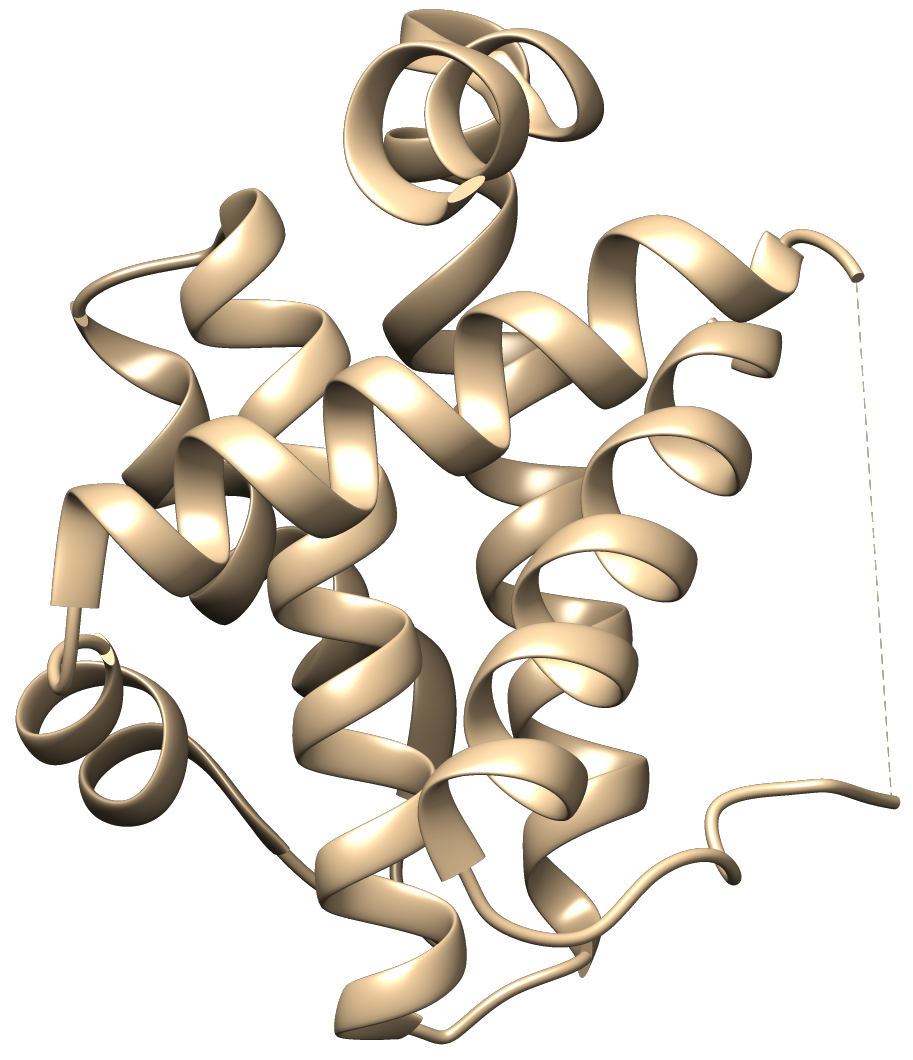
\includegraphics[width=0.48\textwidth]{rysunki/rozdzial_1/bh.png}
	\caption[Struktura domeny BH4]{Wstążkowa reprezentacja domeny BH4 białka Bcl-X$_L$ (kod PDB: \textbf{1AF3}) \cite{Aritomi1997}.}
	\label{fig:bh}
\end{wrapfigure}

\begin{figure}[tb]
\centering
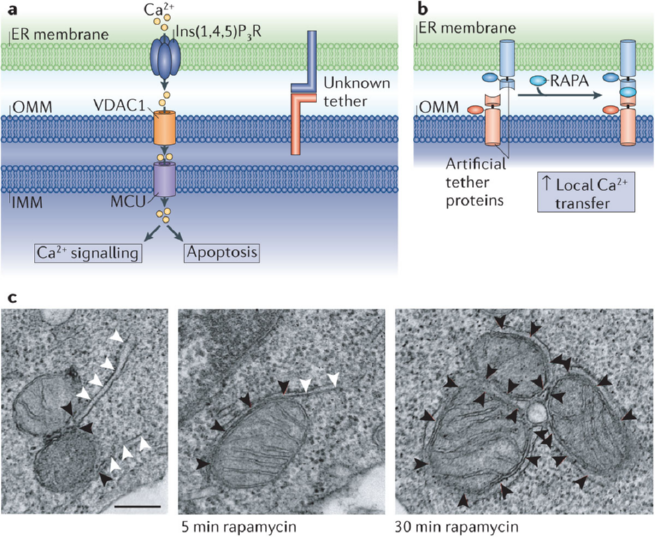
\includegraphics[width=1\textwidth]{rysunki/rozdzial_1/apoptosis_rapa.png}
\caption[Transport jonów Ca$^{2+}$ pomiędzy ER i mitochondriami podczas apoptozy]{ (\textbf{A}) Transport jonów Ca$^{2+}$ pomiędzy retikulum endoplazmatycznym i~mitochondriami podczas wczesnej fazy apoptozy zachodzi w miejscach kontaktu tych dwóch struktur. Szczególną rolę w procesie ustawienia poszczególnych kanałów jonowych w apozycji odgrywają specjalne białka spinające o nieznanym charakterze. (\textbf{B}) Indukcja miejsc wiązania za pomocą białek hybrydowych (opis w tekście) oraz rapamycyny (\textbf{RAPA}); (\textbf{C}) Zdjęcia wykonane transmisyjnym mikroskopem elektronowym komórek RBL-2H3 ze zmodyfikowanymi sztucznymi białkami spinającymi przed i po dimeryzacji indukowanej rapamycyną. Czarne strzałki wskazują miejsca kontaktu ER-mitochondrium, natomiast białe strzałki ER bez kontaktu. Wskaźnik odległości to 250 nm \cite{Rowland2012}.}
\label{fig:apoptoza2}
\end{figure}

Z literatury wynika, że nadmierny napływ jonów wapniowych do mitochondrium powoduje aktywowanie programu apoptozy, czyli uwolnienia białek, które znajdowały się wewnątrz mitochondrium: np. cytochromu C - składnik łańcucha oddechowego, \textbf{AIF} oraz \textbf{Smack/DIABLO}, proteazy serynowe \textbf{HtrA2/Om}i, \textbf{endonukleazę G}. Na kolejnych etapach szlaku apoptotycznego prowadzi to do aktywacji kaspaz efektorowych (kaspazy-3, 6 i 7), które doprowadzają do degradacji białek w~komórce \cite{Desagher2000,Martins2002,Roy2008}. Cytochrom C w cytozolu tworzy duży, niejednorodny kompleks z~białkami Apaf1 i~Apaf2 oraz prokaspazy-9, nazywany apoptosomem. Cytochrom C działa w tym kompleksie jako kofaktor i stymuluje auto oligomeryzacje białka Apaf-1, które z kolei jest aktywatorem prokaspazy-9. Kaspaza-9 uznawana jest za kaspazę inicjatorową mitochondrialnego szlaku apoptotycznego. Na drodze ograniczonej proteolizy może ona aktywować kaspazy wykonawcze (kaspazę-3 lub -7), które aktywują kaskadę innych kaspaz lub rozpoczynają proces degradacji aparatu białkowego \cite{Chang2000,Nicholson1999}. Prokaspaza-3 może również bezpośrednio aktywować polipeptyd AIF, który aktywowany przenosi się do jądra komórkowego i tam aktywuje endonukleazy rozpoczynające degradację DNA \cite{Chang2000,Cohen1997}. 

Uwolnienie cytochromu C i innych białek mitochondrialnych zaangażowanych w~apoptozę regulowane jest przez grupę protein z \textbf{rodziny Bcl-2} (ang. \emph{\textbf{B}-\textbf{c}ell \textbf{l}eukemia/ \textbf{l}ymphoma-\textbf{2}})\nomenclature{Bcl-2}{ang. \textit{\textbf{B}-\textbf{c}ell \textbf{l}eukemia/lymphoma-\textbf{2}}}, których przedstawiciele mogą mieć działanie zarówno proapoptotyczne (Bak, Diva, Bcl-X$_S$, Bik, Bim Bad, Bid, Egl-1), jaki i~antyapoptotyczne (Bcl-2, Bcl-X$_L$, Mcl-1, CED-9, Bcl2A1, Bfl-1, Bcl-2-L2) \cite{Chao1998}. Szczegółowy opis poszczególnych białek znajduje się w Tab.~\ref{tab:bcl}. Białka rodziny Bcl-2 dzielą ze sobą cztery \textbf{domeny BH} (ang. \textit{\textbf{B}cl-2 \textbf{h}omology region})(Ryc.~\ref{fig:bh})\nomenclature{BH}{ang. \textit{\textbf{B}cl-2 \textbf{h}omology region}}, nazwane BH1, BH2, BH3, BH4, które odgrywają znaczną rolę w procesie kontroli apoptozy. W białkach anty-apoptotycznych (Bcl-2 oraz BclX$_L$) wszystkie cztery domeny są konserwowane ewolucyjnie, natomiast białka proapoptotyczne take jak Bad, Bid oraz Bim posiadają tylko jedną domenę - BH3 - i~z~tego powodu wyróżniane są jako podgrupa białek o nazwie ,,\textit{BH3-only}''~\cite{Lomonosova2008}. Czasami, także białka Bax wyodrębniane są z~rodziny Bcl-2 jako osobna podgrupa.

\textbf{Domeny BH} uczestniczą w dimeryzacji poszczególnych przedstawicieli grupy białek Bcl-2. Dimeryzacja może zachodzić na drodze łączenia się białek Bcl-2, wtedy wykorzystywane są zazwyczaj oddziaływania typu ,,\textbf{ogon-głowa}'', kiedy to N-końcowy region białka (zawierający domenę BH4) oddziałuje z dalszym, C-końcowym regionem siostrzanej cząsteczki, w której zlokalizowane są domeny BH1, BH2 oraz BH3. Heterodimeryzacja natomiast polega na łączeniu białek Bcl-2/Bax, kiedy zaangażowane są oddziaływania ,,\textbf{ogon-ogon}'', dzięki możliwość interakcji domen BH1, BH2, BH3 białek Bcl-2 ze środkową częścią Bax, w której znajduje się domena BH3 \cite{Chao1998,Sattler1997}. Homo - i heterodimeryzacja białek z rodziny Bcl-2 wpływa w znaczny sposób na proces uwalniania cytochromu C z mitochondrium i aktywności niektórych kaspaz oraz na proces formowania się i aktywności PTP, co przekłada się na decyzje komórki o~kontynuowaniu, bądź terminacji szlaku apoptotycznego zależnego od mitochondrium.

\begin{figure}[!ht]
  \centering
  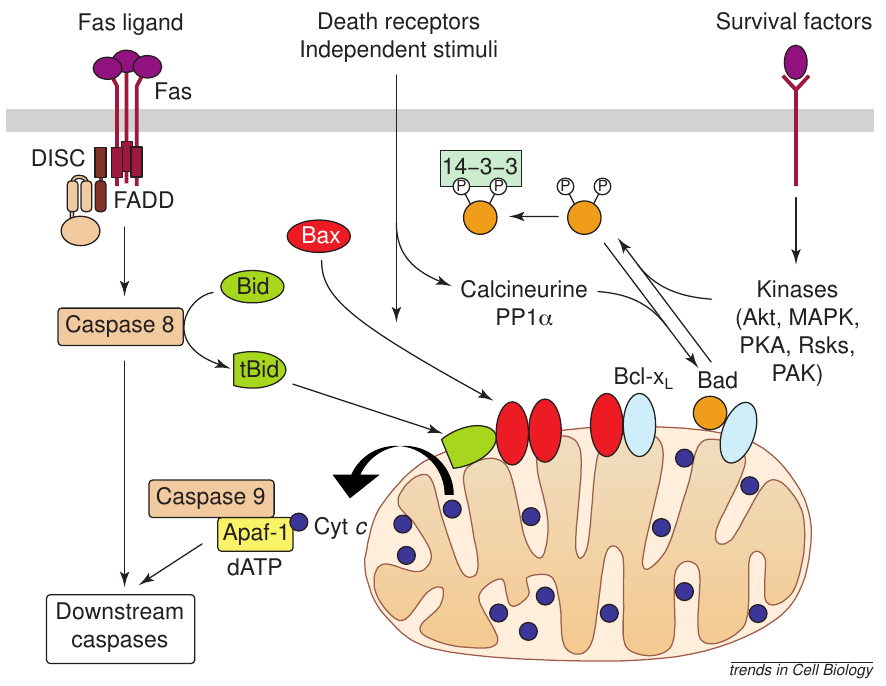
\includegraphics[width=0.9\textwidth]{rysunki/rozdzial_1/apoptosisMitoPath.png}
  \caption [Mitochondrialna ścieżka apoptozy]{Mitochondria stanowią centralny punkt decyzyjny komórki, w którym krzyżują się zewnętrzne i wewnętrzne szlaki apoptotyczne. Wiele ścieżek programowanej śmierci komórki zależna jest od białek rodziny Bcl-2, w szczególności białek grupy ,,BH3-only'' takich jak Bid i Bad~\cite{Leo2005}.}
  \label{fig:apoptosisMitoPath}
\end{figure}


\bigskip

\noindent Działanie niektórych przedstawicieli białek rodziny Bcl-2:

\medskip

\noindent \textbf{Antyapoptotyczne:}
\begin{description}
\item [Bcl-2] Hamuje apoptozę w różnych systemach komórkowych, np. komórkach krwiotwórczych i neuronach. Reguluje śmierć komórek przez kontrolę przepuszczalności błony mitochondrialnej. Hamuje aktywność kaspaz poprzez zapobieganie uwalnianiu cytochromu C z~mitochondriów i/lub przez wiązanie się z czynnikiem aktywującym apoptozę Apaf-1 \cite{Bonneau2013,Kelly2011}.
\item [BclX$_L$] Znajduje się na zewnętrznej błonie mitochondrialnej i reguluje otwarcie kanału VDAC. VDAC reguluje mitochondrialny potencjał błonowy, a więc kontroluje wytwarzanie reaktywnych form tlenu i uwalnianie cytochromu C przez mitochondria, z których oba są silnymi induktorami apoptozy \cite{Cheng1996}.
\item [Bfl-1] Hamuje apoptozę indukowaną IL-3. Może działać w odpowiedzi komórek krwiotwórczych na sygnały zewnętrzne i wspomaga przeżywalności komórek śródbłonka podczas infekcji. Indukowany NF$\kappa$B hamuje aktywność czynnika TNF$\alpha$ \cite{Zong1999}.
\end{description}

\noindent \textbf{Proapoptotyczne:}
\begin{description}
\item [Bak] W obecności odpowiedniego bodźca, przyspiesza programowaną śmierć komórek przez wiązanie do antyapoptotycznego białka Bcl-2 \cite{Scorrano2003}.
\item [Diva] Ekspresja białka Diva hamuje wiązanie Bcl-X$_L$ do kompleksu Apaf-1. Stanowi nowy typ mitochondrialnych czynników proapoptotycznych z rodziny Bcl-2, które promują apoptozę niezależnie od regionu BH3, poprzez bezpośrednie wiązanie do Apaf-1 \cite{Inohara1998}.
\item [Bik] Przyspiesza programowaną śmierć komórki. Wiąże się z represorami apoptozy,np. Bcl-X$_L$, BHRF1, Bcl-2 lub ich homologów. Nie oddziałują z białkami Bax \cite{Tsujimoto2003}.
\item [Bim] Indukuje apoptozę wiążąc się z anty-apoptotycznymi białkami takimi jak Bcl-2, Bcl-X$_L$ i~Mcl-1, hamując ich działanie przeżyciowe \cite{Czabotar2009}.
\item [Bad] Promuje śmierć komórek. Konkuruje z białkiem Bax w wiązaniu do białek antyapoptotycznych: Bcl-X$_L$, Bcl-2 i Bcl-2-L2/Bcl-W, w ten sposób wpływając na poziom heterodimeryzacji tych białek z Bax. Działa jako łącznik pomiędzy zewnętrznymi i wewnętrznymi ścieżkami programowanej śmierci \cite{Gibson1996}.
\item [Bid] Produkt proteolizy tBid umożliwia uwolnienie cytochromu C. Przeciwdziała działaniu ochronnemu białka Bcl-2 \cite{Galluzzi2012,Hajnoczky2003}.
\item [Bax] W warunkach stresu, ulega zmianom konformacyjnym, które powodują jego przemieszczenie do błony mitochondriów, gdzie oddziałuje z poryną VDAC. Co ostatecznie prowadzi do uwolnienia cytochromu C \cite{Gautier2011,Scorrano2003}.
\end{description}

\begin{table}[!ht]
\small
\centering
\begin{tabular}{lp{6.1cm}p{3.9cm}r}
\toprule[0.12em]
\textbf{Symbol} & \textbf{Pełna nazwa białka} & \textbf{Domeny BH} & \textbf{Referencje} \\ \midrule[0.06em]
\multicolumn{4}{>{\columncolor[gray]{.9}}c}{\rule[-2ex]{0pt}{5.5ex}\textbf{Anty-apoptotyczne}}\\[0.08em]
\rule[-2ex]{0pt}{5.5ex}	\textbf{Bcl-2} & \textit{\textbf{B}-\textbf{c}ell \textbf{l}eukemia/lymphoma-\textbf{2}} & BH1, BH2, BH3, BH4 & \cite{Kelly2011} \\
\textbf{Bcl-2-L2} & Bcl-2-like protein 2-\textbf{l}ike protein \textbf{2}& \nomenclature{Bcl-2-L2}{ang. \textit{Bcl-2-like protein 2-\textbf{l}ike protein \textbf{2}}} & \cite{Gibson1996}\\
\rule[-2ex]{0pt}{5.5ex}	\textbf{Bcl-$X_L$} & \textit{\textbf{B}-\textbf{c}ell \textbf{l}ymphoma-e\textbf{x}tra \textbf{l}arge}\nomenclature{Bcl-$X_L$}{ang. \textit{\textbf{B}-\textbf{c}ell \textbf{l}ymphoma-e\textbf{x}tra \textbf{l}arge}} & BH1, BH2, BH3, BH4 &  \cite{Ban1998,Cheng1996}  \\
\rule[-2ex]{0pt}{5.5ex}	\textbf{Mcl-1}   & \textit{\textbf{M}yeloid \textbf{c}ell \textbf{l}eukemia sequence \textbf{1}}\nomenclature{Mcl-1}{\textit{\textbf{m}yeloid \textbf{c}ell \textbf{l}eukemia sequence \textbf{1}}} & BH1, BH2, BH3, BH4 & \cite{Perciavalle2013} \\
\rule[-2ex]{0pt}{5.5ex}	\textbf{CED-9} & \textit{\textbf{Ce}ll \textbf{d}eath protein 9}\nomenclature{CED-9}{ang. \textit{\textbf{ce}ll \textbf{d}eath protein 9}}                                     & BH1, BH2, BH3, BH4 & \cite{Hengartner1994} \\
\rule[-2ex]{0pt}{5.5ex}	\textbf{Bcl2A1} & \textit{\textbf{Bcl2}-related protein \textbf{A1}}\nomenclature{Bcl2A1}{\textit{\textbf{Bcl2}-related protein \textbf{A1}}} & BH1, BH2, BH3, BH4 & \cite{Haq2013}\\
\rule[-2ex]{0pt}{5.5ex}	\textbf{Bfl-1} & \textbf{B}cl related \textbf{f}etal \textbf{l}iver homolog - \textbf{1}\nomenclature{Bfl-1}{ang. \textit{\textbf{B}cl related \textbf{f}etal \textbf{l}iver homolog-\textbf{1}}} & BH1, BH2, BH3, BH4 & \cite{Zhang2000,Zong1999} \\
\multicolumn{4}{>{\columncolor[gray]{.9}}c}{\rule[-2ex]{0pt}{5.5ex}\textbf{Pro-apoptotyczne}} \\[0.12em]
\rule[-2ex]{0pt}{5.5ex}	\textbf{Bak} & \textit{\textbf{B}cl-2 homologous \textbf{a}ntagonist \textbf{k}iller}\nomenclature{Bak}{ang. \textit{\textbf{B}cl-2 homologous \textbf{a}ntagonist \textbf{k}iller}} & BH1, BH2, BH3 & \cite{Chao1998} \\
\rule[-2ex]{0pt}{5.5ex}	\textbf{Diva} & \textit{\textbf{D}eath \textbf{i}nducer binding to \textbf{v}Bcl-2 and \textbf{A}paf-1}\nomenclature{Diva}{ang. \textit{\textbf{D}eath \textbf{i}nducer binding to \textbf{v}Bcl-2 and \textbf{A}paf-1}} & BH1, BH2, BH3, BH4 & \cite{Inohara1998}\\
\rule[-2ex]{0pt}{5.5ex}	\textbf{Bcl-X$_S$} & \textit{\textbf{B}-\textbf{c}ell \textbf{l}ymphoma-e\textbf{x}tra \textbf{s}mall} \nomenclature{Bcl-X$_S$}{ang. \textit{\textbf{B}-\textbf{c}ell \textbf{l}ymphoma-e\textbf{x}tra \textbf{s}mall}}& BH3, BH4 & \cite{Ban1998,Chang1999} \\
\rule[-2ex]{0pt}{5.5ex}	\textbf{Bik} & \textit{\textbf{B}cl-2-\textbf{i}nteracting \textbf{k}iller}\nomenclature{Bik}{ang. \textit{\textbf{B}cl-2-\textbf{i}nteracting \textbf{k}iller}} & BH3 & \cite{Dunham1999}\\
\rule[-2ex]{0pt}{5.5ex}	\textbf{Bim} & \textit{\textbf{B}cl-2-\textbf{i}nteracting \textbf{m}ediator of cell death}\nomenclature{Bim}{ang. \textit{\textbf{B}cl-2-\textbf{i}nteracting \textbf{m}ediator of cell death}} & BH3 & \cite{Gogada2013,O'Connor1998}\\
\rule[-2ex]{0pt}{5.5ex}	\textbf{Bad} & \textit{\textbf{B}cl-2-\textbf{a}ssociated \textbf{d}eath promoter}\nomenclature{Bad}{ang. \textit{\textbf{B}cl-2-\textbf{a}ssociated \textbf{d}eath promoter}} & BH3 & \cite{Adachi2002} \\
\rule[-2ex]{0pt}{5.5ex}	\textbf{Bid} & \textit{\textbf{B}cl-2 \textbf{i}nteracting \textbf{p}rotein}\nomenclature{Bid}{ang. \textit{\textbf{B}cl2 \textbf{i}nteracting \textbf{p}rotein}} & BH3 & \cite{Luo1998} \\
\rule[-2ex]{0pt}{5.5ex}	\textbf{Egl-1} & \textbf{Eg}g \textbf{l}aying abnormal-1\nomenclature{Egl-1}{ang. \textit{\textbf{Eg}g \textbf{l}aying abnormal-1}} & BH3 & \cite{Conradt1998} \\
\rule[-2ex]{0pt}{5.5ex}	\textbf{Bax} & \textit{\textbf{B}cl-2-\textbf{a}ssociated \textbf{X} protein}\nomenclature{Bax}{białka powiązane z Bcl-2 (ang. \textit{\textbf{B}cl-2-\textbf{a}ssociated \textbf{X} protein})} & BH1, BH2, BH3 & \cite{Czabotar2009,Yao2014} \\ \bottomrule[0.12em]
\end{tabular}
\caption[Białka rodziny Bcl-2]{Białka rodziny Bcl-2 - udział poszczególnych domen BH w strukturze.}
\label{tab:bcl}
\end{table}

%o charakterze pro-apoptotycznym z rodziny Bcl-2 i białek rodziny Bax i Bak (ang. \textit{\textbf{B}cl-2 homologous \textbf{a}ntagonist \textbf{k}iller})\nomenclature{Bak}{ang. \textit{\textbf{B}cl-2 homologous \textbf{a}ntagonist \textbf{k}iller}}. Bax w większości znajduje się w cytozolu. Białka te znajdują się w stanie nieaktywnym w komórkach zdrowych. Aktywacja szlaku apoptozy prowadzi do uruchomienia kaskady szeregu białek z rodziny Bcl-2, których przedstawiciele mogą mieć działanie zarówno pro- (Bax, Bak, Diva, Bcl-X$_S$, Bik, Bim Bad, Bid, Egl-1), jaki i anty-apoptotyczne (Bcl-2, Bcl-X$_L$, Mcl-1, CED-9, Bcl2A1, Bfl-1)(Tab.~\ref{tab:bcl}).


Proteoliza białka Bid łączy zewnętrzną ścieżkę apoptotyczna ze ścieżką mitochondrialną. Umożliwia to przekazanie zewnętrznych sygnałów apoptozy płynących z receptorów błonowych na szlak aktywujący mitochondrialny mechanizm śmierci. Skrócony polipeptyd Bid, czyli tBid (ang. \textbf{t}runctated \textbf{Bid}) wiąże się z białkiem Bax, doprowadzając do zmian konformacyjnych jego N-końca, co umożliwia Bax przyłączanie do powierzchni mitochondriów. Tam oddziałuje z~poryną VDAC przy tworzeniu megakanału PTP. Efektem jest oligomeryzacja białek Bax i~Bak na zewnętrznej błonie mitochondrialnej (Ryc.~\ref{fig:apoptosisMitoPath}), co poprzedza wyrzut wymienionych wcześniej czynników apoptotycznych do cytozolu \cite{Scorrano2003,Tsujimoto2003}. Mitochondria stanowią więc centralny ,,punkt decyzyjny'', w którym zbiegają się najważniejsze szlaki prowadzące do apoptozy \cite{Desagher2000,Leo2005}.

\begin{sidewaysfigure}[p]
\centering
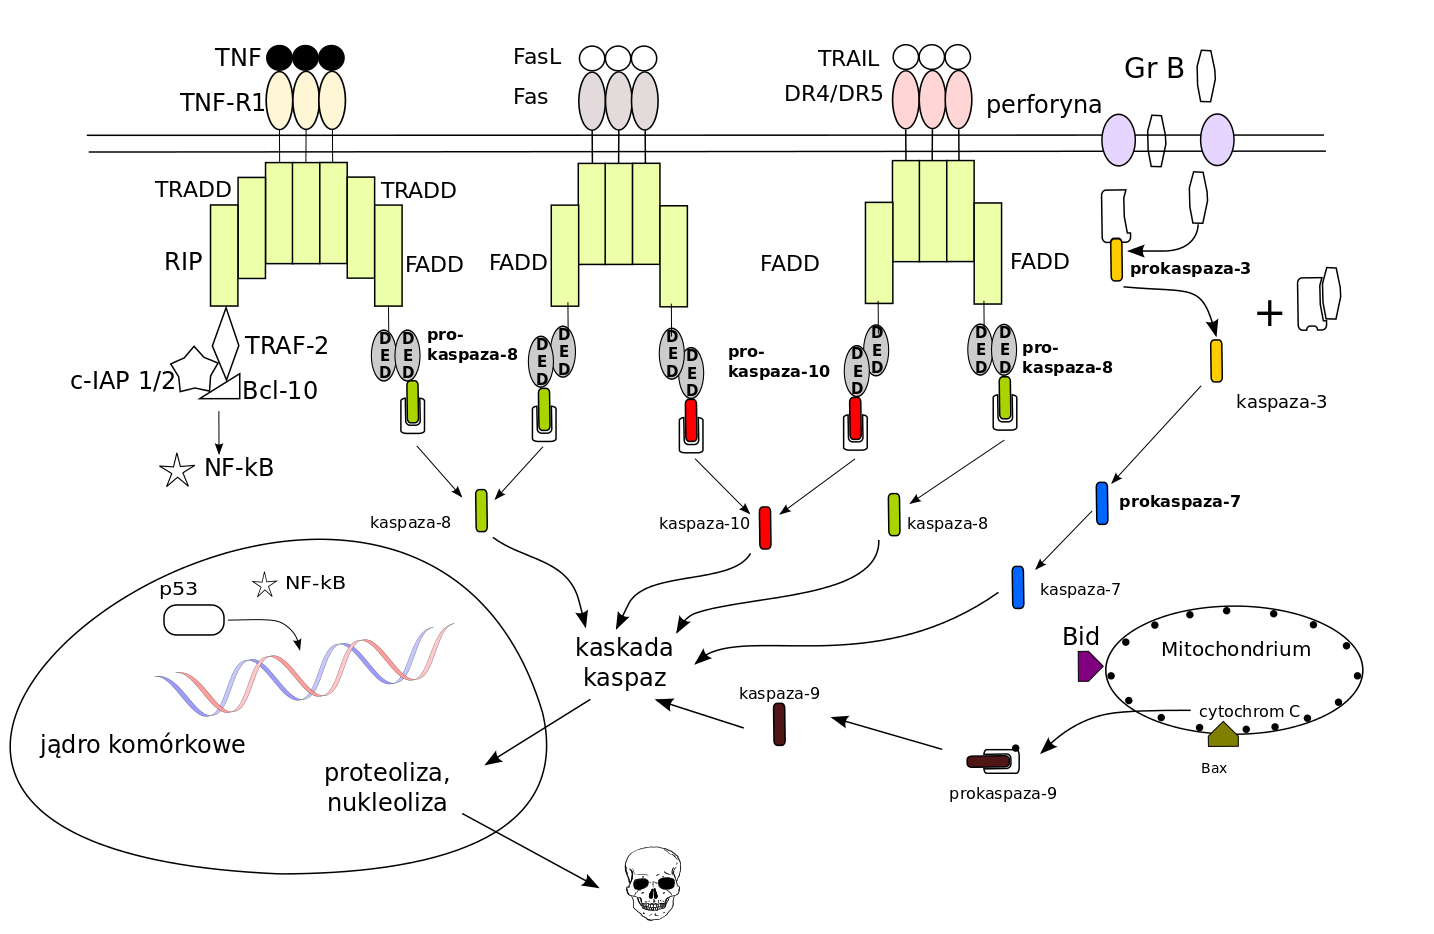
\includegraphics[width=0.95\textwidth]{rysunki/rozdzial_1/apoptoza.png}
\caption[Uproszczony schemat szlaków apoptotycznych]{Uproszczony schemat głównych szlaków apoptotycznych \cite{Desagher2000}.}
\label{fig:apoptoza}
\end{sidewaysfigure}

Istnieje jeszcze jeden szlak apoptotyczny, niezależny od sygnalizacji receptorów powierzchniowych, czy mitochondriów, który jest uruchamiany w retikulum endoplazmatycznym w wyniku działania czynników stresogennych. Stres powoduje nagromadzenie się jonów wapnia w~retikulum, co destabilizuje funkcjonowanie białek wspomagających prawidłowe zwijanie innych protein - chaperonów, co doprowadza do nagromadzenia się nieprawidłowo zwiniętych białek w~ER.

\FloatBarrier
\section{Rola Ca$^{2+}$ w zapłodnieniu}

Rola jonów wapnia związana z aktywacją oocytów podczas procesu zapłodnienia znana jest od lat 90-tych poprzedniego wieku. Natomiast dopiero niedawno zaczęto gromadzić informacje dotyczące znaczenia Ca$^{2+}$ podczas aktywacji plemników przed zapłodnieniem~\cite{Sardet2007}.

\begin{figure}[tb]
\centering
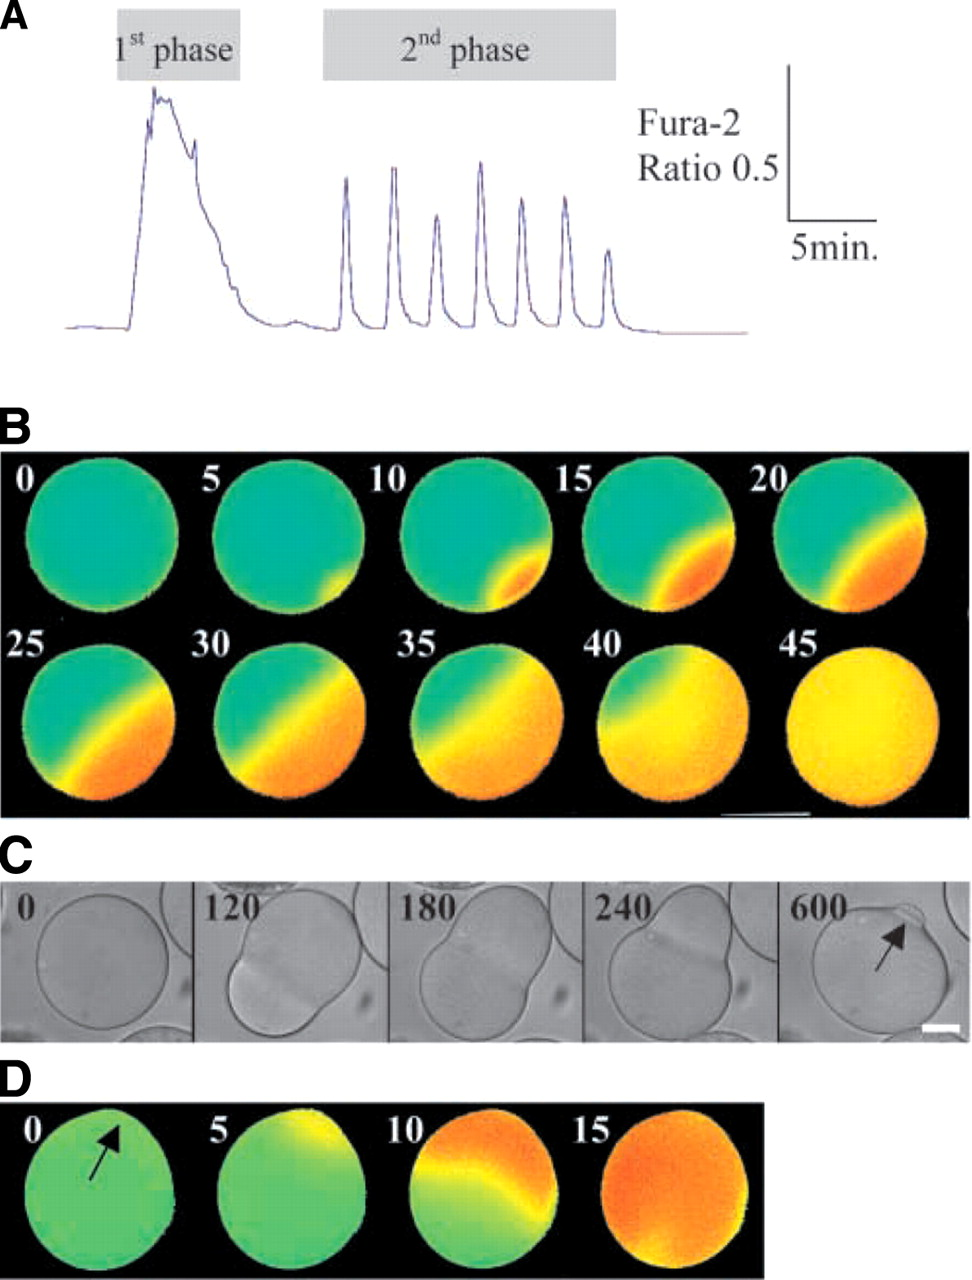
\includegraphics[scale=0.4]{rysunki/rozdzial_1/zaplodnienie.jpg}
\caption [Fale wapniowe - zapłodnienie]{Fale wapniowe przechodzące przez oocyt podczas procesu zapłodnienia. (\textbf{A}) czasowa charakterystyka poszczególnych fal wapniowych w oocycie podczas zapłodnienia. Widoczna jest jedna duża fala wapniowa, po której następuje siedem mniejszych. (\textbf{B}) fala wapniowa pierwszej fazy, rozpoczynająca się w punkcie wniknięcia plemnika. Fuzja gamet prowadzi do powstania dużej fali wapniowej, która w~ciągu 40 sekund obejmuje cały oocyt. (\textbf{C}) reorganizacja struktury wewnętrznej oocytu i wytworzenie "kurczliwego bieguna", z którego biorą początek kolejne fale wapniowe. (\textbf{D}) fala wapniowa  podczas drugiej fazy, rozchodząca się z bieguna kurczliwego~\cite{Whitaker2006}.}
\label{fig:zaplodnienie}
\end{figure}

Początek nowego życia zaczyna się od wymiany szeregu informacji, w których kluczową rolę odgrywa wapniowa ścieżka sygnalizacyjna. Wapń odgrywa rolę kluczowego przekaźnika, który wymienia informacje pomiędzy gametami. Gdy plemnik zbliża się do powierzchni komórki jajowej obie gamety ulegają aktywacji za sprawa zmian stężenia wolnych jonów wapnia, które z~kolei zmieniają metabolizm obu gamet \cite{Campbell2006}. Zmiany cytozoliczne oocytu zachodzą poprzez aktywację receptora IP$_3$. Plemniki ssaków aktywują się tuż przed zapłodnieniem i również w~tym procesie wapń odgrywa znaczącą rolę. Wzrost stężenia tych jonów w części ogonkowej plemnika doprowadza do wzrostu częstotliwości ,,ruchów'' włókien kurczliwych. Zwiększa to ruchliwość plemnika, który jest wtedy w stanie pokonać opór środowiska (wyściółkę śluzową macicy, osłonkę przejrzystą). Wyrzut jonów wapnia w oocycie odbywa się dzięki aktywacji enzymu - fosfolipazy typu C (PLC) za pomocą czynnika aktywującego - tzw. \textbf{PLC$\zeta$} pochodzącego z~plemnika i wzrostu stężenia IP$_3$ wewnątrz komórki jajowej \cite{Swann2013,Yu2012}. Wzrost stężenia IP$_3$ wyzwala serię fal wapniowych w oocycie (Ryc.~\ref{fig:zaplodnienie}). Późniejsze zmiany stężenia wapnia służą jako wyznaczniki kolejnych podziałów komórkowych oraz jako sygnały to powstawania wzorców \textbf{gastrulacji} i \textbf{organogenezy}, współtworząc program rozwojowy zarodków. Dodatkowo, w~przypadku komórki jajowej, w chwili zapłodnienia do cytozolu uwalniane są jony wapnia, które mogą wywołać pojedynczą falę wapniową bądź szereg oscylacji jonów wapnia. Powstanie pojedynczej lub wielokrotnej fali wapniowej jest cechą specyficzną gatunkowo. Fala ta jest sygnałem, który ma na celu ustawienie fazy cyklu komórkowego oocytu i wyrzut ziarnistości znajdujących się pod błoną komórkową. Zawartość pęcherzyków zmienia skład chemiczny otoczki oocytu i~uniemożliwia przyłączenie się kolejnego plemnika \cite{Gonzalez-Garcia2013,Swann2008}.

\section{Homeostaza wapniowa w komórce}



\begin{wraptable}{r}{0.55\textwidth}
\centering
\begin{tabular}{ccc}\toprule[0.12em]
\rule[-2ex]{0pt}{5.5ex} \multirow{2}{*}{\textbf{Jon}} & \multicolumn{2}{c}{\textbf{Stężenie [mM]}}\\\cline{2-3}
\rule[-2ex]{0pt}{5.5ex} & \textbf{W cytozolu} & \textbf{Poza komórką} \\\midrule[0.06em]
\rule[-2ex]{0pt}{5.5ex} K$^+$ & 140 & 4 \\
\rule[-2ex]{0pt}{5.5ex} Na$^+$ & 14 & 440 \\
\rule[-2ex]{0pt}{5.5ex} Cl$^-$ & 4 & 116 \\
\rule[-2ex]{0pt}{5.5ex} \ce{HCO_3^-} & 12 & 29 \\
\rule[-2ex]{0pt}{5.5ex} Mg$^{2+}$ & 0.8 & 1.5 \\
\ngray \rule[-2ex]{0pt}{5.5ex} Ca$^{2+}$ & <0.0002 & 2 \\ \bottomrule[0.12em]
\end{tabular}
\caption[Stężenie jonów w komórce]{Stężenie jonów w komórce i macierzy zewnątrzkomórkowej \cite{Lodish2000}.}
\label{tab:jony}
\end{wraptable}

Badania ostatnich lat wykazują, że jony wapnia stanowią kluczową rolę w przekazywaniu informacji w komórkach eukariotycznych. Stężenia Ca$^{2+}$ w komórce jest niskie i rośnie gwałtownie dopiero w wyniku pobudzenia. Podwyższone stężenie wapnia w~komórce uruchamia różnego rodzaju kaskady zdarzeń, które prowadzą do aktywacji wielu szlaków przekaźnictwa sygnału w komórce i określonej odpowiedzi komórki. Wapń spełnia więc klasyczną definicję wtórnego \textbf{przekaźnika informacji}. Stężenie Ca$^{2+}$ w cytozolu, w~komórce niepobudzonej jest bardzo niskie i wynosi około 50-100 nM, natomiast w przestrzeni zewnątrzkomórkowej poziom tego jonu wynosi 1-2 mM. Różnica pomiędzy cytozolem a płynami ustrojowymi jest więc gigantyczna. Stężenie jonu po obu stronach błony komórkowej różni się niemal dziesięć tysięcy razy (Tab.~\ref{tab:jony}). W wyniku pobudzenia komórki stężenie Ca$^{2+}$ cytozolicznego wzrasta dziesięciokrotnie do 1-2 $\mu$M. Przy tak dużej różnicy stężeń utrzymanie stałego, niskiego poziomu Ca$^{2+}$ w komórce realizowane jest za pomocą układów białek transportujących wapń, takich jak: pompy, kanały, czy wymienniki, przez które Ca$^{2+}$ jest usuwany na zewnątrz lub magazynowany w organellach wewnątrzkomórkowych (Ryc~\ref{fig:toolkit}). Ogół procesów prowadzących do utrzymania stałego, niskiego stężenia Ca$^{2+}$, które pozostaje w dynamicznej równowadze nosi nazwę \textbf{homeostazy wapniowej}.

\begin{table}[t]
\large
\centering
\begin{tabular}{lcc}\toprule[0.12em]
\rule[-2ex]{0pt}{5.5ex} \multirow{2}{*}{\textbf{Kompartment}} & \multicolumn{2}{c}{\textbf{Stężenie [$\mu$M]}}\\\cmidrule{2-3}
\rule[-2ex]{0pt}{5.5ex} & \textbf{Spoczynek} & \textbf{Aktywacja} \\\midrule[0.06em]
\rule[-2ex]{0pt}{5.5ex} Cytozol & \textcolor{blue}{\textbf{0.05--0.1}} & \textcolor{red}{\textbf{0.5--2}} \\
\rule[-2ex]{0pt}{5.5ex} ER & \textcolor{blue}{\textbf{0.5}} & \textcolor{red}{\textbf{\textbf{0.1}}} \\
\rule[-2ex]{0pt}{5.5ex} Mitochondria & \textcolor{blue}{\textbf{\textbf{0.2}}} & \textcolor{red}{\textbf{1--500}} \\
\rule[-2ex]{0pt}{5.5ex} Jądro komórkowe & \textcolor{blue}{\textbf{0.1}} & \textcolor{red}{\textbf{2}} \\
\rule[-2ex]{0pt}{5.5ex} Aparat Golgiego & \textcolor{blue}{\textbf{0.3}} & \textcolor{red}{\textbf{0.2}} \\
\rule[-2ex]{0pt}{5.5ex} Przestrzeń zewnątrzkomórkowa & \textcolor{blue}{\textbf{2000}} & \textcolor{red}{\textbf{$\sim$2000}} \\ \bottomrule[0.12em]
\end{tabular}
\caption[Stężenie jonów wapnia w kompartmentach]{Stężenie jonów wapnia w poszczególnych kompartmentach komórek eukariotycznych w czasie \textcolor{blue}{spoczynku} i w wyniku \textcolor{red}{aktywacji sygnalizacji wapniowej} \cite{Laude2009}.}
\label{tab:caakt}
\end{table}

Nadmiar Ca$^{2+}$ usuwany jest z cytozolu na zewnątrz, tj. w kierunku wyższego stężenia, przez enzymy błony plazmatycznej Ca$^{2+}$-ATPazy, zwane także pompami wapniowymi (PMCA). Proces ten odbywa się kosztem energii uzyskiwanej z hydrolizy ATP (ATP/Ca$^{2+}$ = 1:1). Innym mechanizmem usuwania Ca$^{2+}$ są tzw. transportery drugiego rzędu, czyli wymienniki sodowo-wapniowe i sodowo-potasowo-wapniowe, będące białkami błonowymi, transportującymi jony sodu i/lub potasu na wymianę z~jonami wapnia (Na$^+$K$^+$/Ca$^{2+}$ = 3:1). Wapń jest także magazynowany w~organellach wewnątrzkomórkowych takich jak mitochondria oraz siateczka śródplazmatyczna. Dodatkowo w~każdym z~kompartmentów występują też swoiste białka buforujące, które bardzo wydajnie wiążą wolne jony wapnia (Rozdz.~\ref{ss:bufory}). Do siateczki śródplazmatycznej Ca$^{2+}$ pompowany jest przez kolejną Ca$^{2+}$-ATPazę (SERCA), różniącą się od tej występującej w~błonie plazmatycznej przede wszystkim wydajnością (ATP/Ca$^{2+}$ = 1:2). Jony Ca$^{2+}$ zmagazynowane wewnątrz siateczki również wiązane są z określonymi białkami buforującymi: kalsekwestryną i~kalretikuliną (Tab.~\ref{tab:cabp}). Wapń magazynowany jest również w mitochondriach, aparacie Golgiego i jądrze komórkowym. Transport wapnia do mitochondriów - drugiego pod względem znaczenia magazynu jonów wapniowych w~komórce, kontrolowany jest przez multimeryczne białko - uniporter mitochondrialny, opisany szczegółowo w rozdziale~\ref{ss:uniporter}. Transport jonów na zewnątrz kontrolują mitochondrialne wymienniki sodowo-wapniowe. Szczegółowy opis mechanizmów transportu jonów wapnia -z i -do magazynów retikularnych i mitochondrialnych znajduje się w~rozdziałach~\ref{ss:transportER} i~~\ref{ss:transportmito}. Wymienione wyżej mechanizmy współuczestniczą w zachowaniu homeostazy wapniowej w komórce i pozwalają na zachowanie stałego stężenia tych jonów w cytozolu (w~wysokich stężeniach Ca$^{2+}$ jest cytotoksyczny). 

W komórkach niepobudliwych mobilizacja Ca$^{2+}$ w komórce ma charakter dwufazowy. Pierwszą fazę stanowi opisany w rozdziale \ref{ss:metabo} szlak sygnalizacyjny, w którym aktywacja receptora metabotropowego, sprzężonego z białkiem G prowadzi do aktywacji fosfolipazy C, produkcji IP$_3$ i uwolnienia jonów wapnia z magazynów wewnątrzkomórkowych. Komórki pobudliwe charakteryzują się tym, że odpowiednie kanały jonowe - bramkowane ligandem, bądź napięciem znajdują się w ich błonie komórkowej i odpowiedni sygnał aktywuje napływ jonów wapnia ze środowiska zewnątrzkomórkowego do cytozolu. Jak już wspomniano stężenie jonów wapnia w cytozolu jest niskie i wynosi $\sim$~50 - 100 nM. Podczas aktywacji wzrasta średnio dziesięciokrotnie do 1-2 $\mu$M. Siateczka śródplazmatyczna jest magazynem jonów wapna, więc pobudzenie powoduje ich uwolnienie, co oznacza, że stężenie tych jonów spada z 0.5 $\mu$M do 0.1 $\mu$M. Mitochondria w stanie spoczynkowym akumulują niewielkie ilości Ca$^{2+}$ (0.2 $\mu$M), ale podczas aktywacji sa w stanie bardzo wydajnie akumulować uwolnione do cytozolu jony wapnia i stężenie ich rośnie w macierzy mitochondrialnej do 1 $\mu$M. W ekstremalnych przypadkach mitochondria mogą pomieścić o wiele większe ilości tych jonów - nawet do 500 $\mu$M. Stężenie wapnia w pozostałych kompartmentach przed pobudzeniem i w trakcie aktywacji przedstawiono w Tab.~\ref{tab:caakt}~\cite{Laude2009}. 

%Stężenie wapnia w nieaktywowanej komórce utrzymywana jest na bardzo niskim poziomie, ale w wyniku aktywacji dochodzi do jego nagłego podwyższenia. Wahania poziomu wapnia, uaktywniają dalsze etapy kaskady sygnałowej - od aktywacji specyficznych kinaz do otwarcia różnych kanałów w błonie komórkowej.

\begin{figure}[tb]
\centering
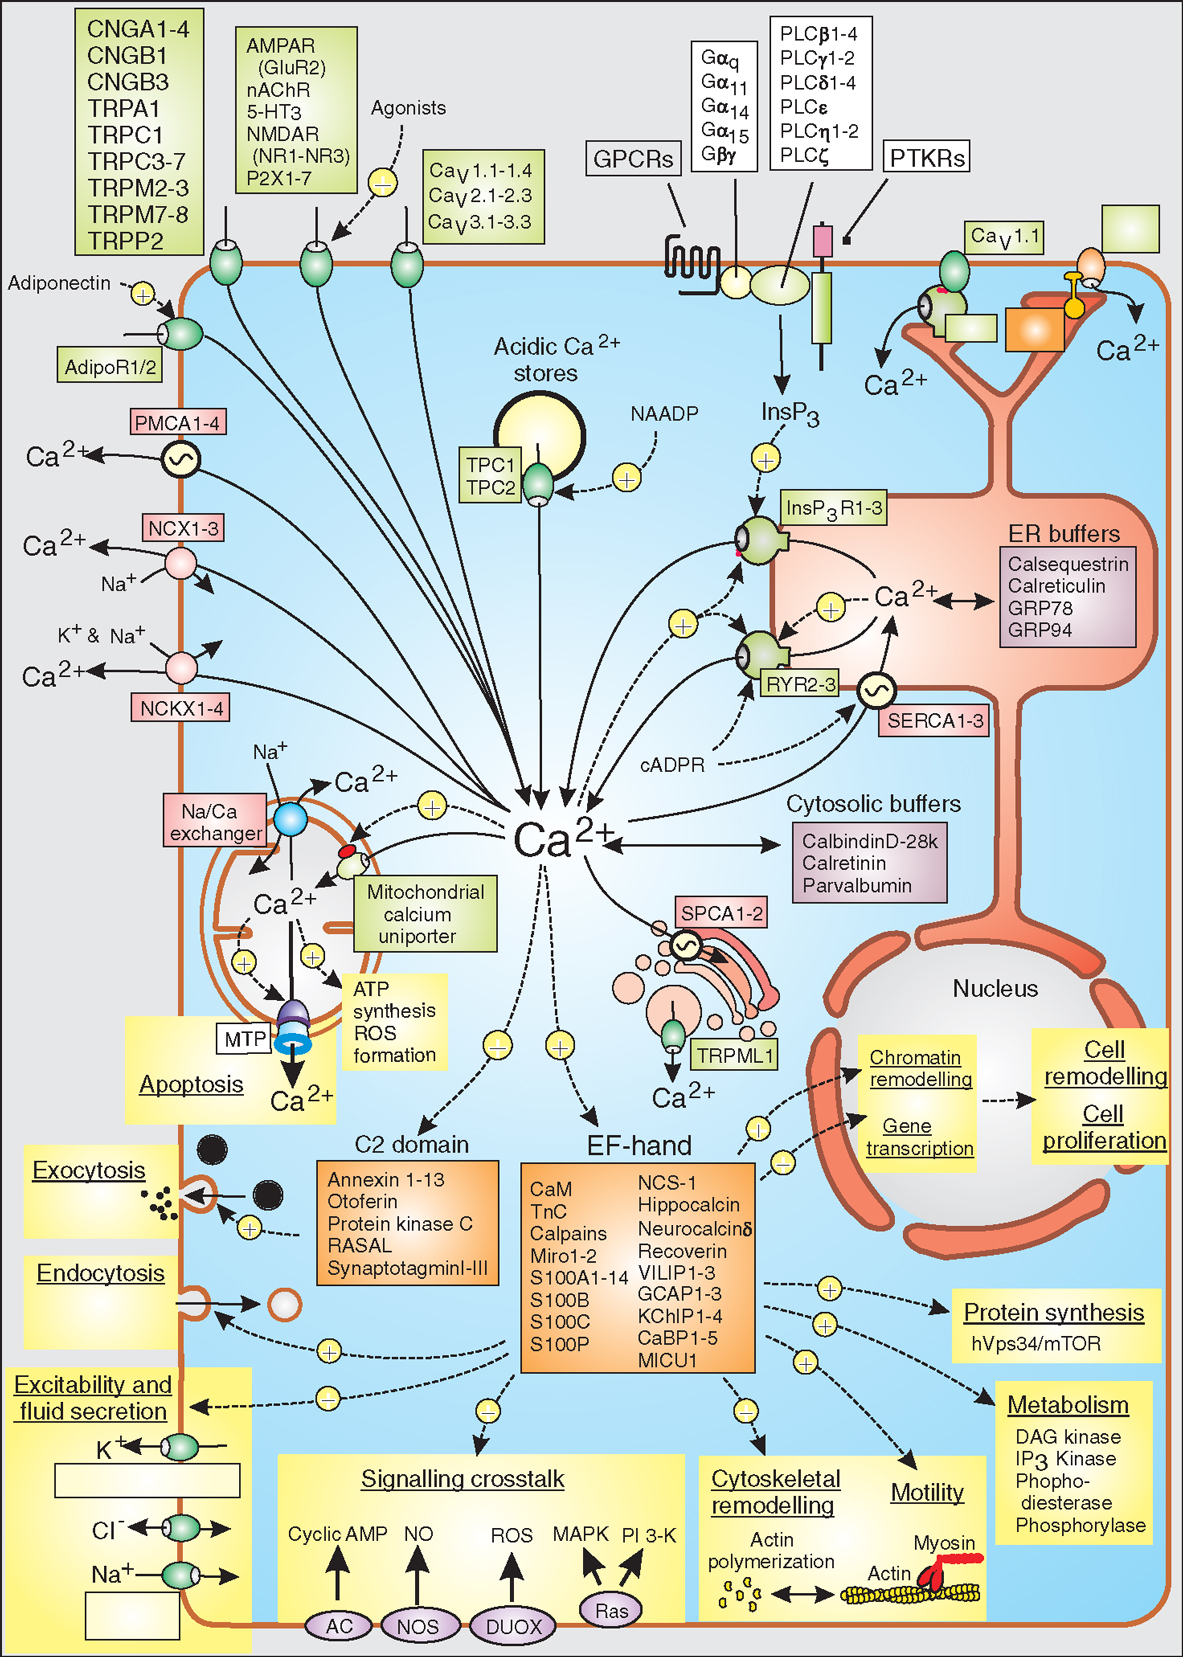
\includegraphics[width=1\textwidth]{rysunki/rozdzial_1/toolkit.jpg}
\caption [Mechanizmy komórkowe zaangażowane w transport Ca$^{2+}$]{Mechanizmy komórkowe zaangażowane w transport Ca$^{2+}$ \cite{Berridge2012b,Clapham2007}.}
\label{fig:toolkit}
\end{figure}




\FloatBarrier
\subsection{Bufory i sensory wapniowe}\label{ss:bufory}
Stężenie wolnych jonów wapnia w cytozolu utrzymywane jest na niskim poziomie także przez odwracalne i selektywne wiązanie tych jonów przez wielkocząsteczkowe białka lub nieorganiczne związki chemiczne. Białka takie określane sa ogólnie jako CaBP (ang. \textbf{ca}lcium \textbf{b}inding \textbf{p}roteins). Wydajność wiązania Ca$^{2+}$ pozwala na zaszeregowanie do jednej z grup, określanych jako - \textbf{bufory wapniowe} lub \textbf{sensory wapniowe} (Tab.~\ref{tab:cabp}). Bufory to bardzo zróżnicowana grupa związków, których zadaniem jest związać jak największą ilość jonów wapnia. Z reguły robią to za pomocą sił elektrostatycznych, eksponując na powierzchni negatywnie naładowane reszty aminokwasowe, które oddziałują z dodatnio naładowanymi jonami wapnia. Sensory służą jako cząsteczki wykrywające obecność jonów wapnia. Zdolność do wykrywania lub buforowania wolnych jonów wapnia zależy od poziomu ekspresji i kombinacji wielu rodzajów białek wiążących wapń obecnych w komórce, przez co poziom związanych i~wolnych jonów wapnia w różnych typach komórek kształtuje się bardzo różnorodnie. Na przykład komórki Purkinjego - neurony występujące w korze móżdżku - charakteryzują się bardzo wysokim poziomem parvalbuminy i kalbindyny, co w efekcie powoduje, że na każdy jon wolnego wapnia przypada około 2000 zbuforowanych. W innych komórkach stosunek ten utrzymuje się w przedziale 50 -- 100:1. Sygnał wapniowy w cytozolu jest bardzo niski. Motoneurony np. mają bardzo niewielkie możliwości buforowania wapnia, co w~konsekwencji daje znaczny wzrost poziomu wapnia w cytozolu podczas sygnalizacji. 


\begin{table}[ht]
\footnotesize
\centering
\begin{tabular}{p{3.1cm}cccc}
	\toprule[0.12em]
	                     & \textbf{M. molowa} & \textbf{Liczba} &     \textbf{Ilość}       &    \textbf{Stała}    \\
	                     & \textbf{monomeru} & \textbf{motywów} &     \textbf{związanych}     & \textbf{dysocjacji} \\
	                     &  \textbf{[kDa]}  & \textbf{\textcolor{LimeGreen}{EF-hand}/\textcolor{blue}{C2}}&   \textbf{jonów Ca$^{2+}$}    &    \textbf{K$_d$[M]} \\ \midrule[0.06em]
\ngray                    \multicolumn{5}{c}{\textbf{Sensory}} \rule[-2ex]{0pt}{5.5ex}	                    \\
	\rule[-2ex]{0pt}{5.5ex} \textcolor{LimeGreen}{kalmodulina}  & \textcolor{LimeGreen}{17} & \textcolor{LimeGreen}{4} & \textcolor{LimeGreen}{4} & \textcolor{LimeGreen}{10$^{-6}$} \\
	\rule[-2ex]{0pt}{5.5ex} \textcolor{LimeGreen}{S100}      & \textcolor{LimeGreen}{12} & \textcolor{LimeGreen}{4} & \textcolor{LimeGreen}{4} & \textcolor{LimeGreen}{10$^{-6}$ -- 10$^{-7}$} \\
	\rule[-2ex]{0pt}{5.5ex} \textcolor{LimeGreen}{kalcyneuryna}  & \textcolor{LimeGreen}{80} & \textcolor{LimeGreen}{4} & \textcolor{LimeGreen}{4} & \textcolor{LimeGreen}{10$^{-6}$ -- 10$^{-7}$} \\
	\rule[-2ex]{0pt}{5.5ex} \textcolor{LimeGreen}{NCS}      & \textcolor{LimeGreen}{22} & \textcolor{LimeGreen}{4} & \textcolor{LimeGreen}{2} & \textcolor{LimeGreen}{5-10$^{-6}$} \\
	\rule[-2ex]{0pt}{5.5ex} \textcolor{LimeGreen}{parvalbumina}  & \textcolor{LimeGreen}{12} & \textcolor{LimeGreen}{3} & \textcolor{LimeGreen}{2} & \textcolor{LimeGreen}{10$^{-7}$} \\
	\rule[-2ex]{0pt}{5.5ex} \textcolor{LimeGreen}{kalbindyna-D28k}& \textcolor{LimeGreen}{28} & \textcolor{LimeGreen}{6} & \textcolor{LimeGreen}{4} & \textcolor{LimeGreen}{10$^{-5}$ -- 10$^{-6}$} \\
	\rule[-2ex]{0pt}{5.5ex} \textcolor{LimeGreen}{kalbindyna-D9k} & \textcolor{LimeGreen}{9} & \textcolor{LimeGreen}{2} & \textcolor{LimeGreen}{2} & \textcolor{LimeGreen}{10$^{-3}$ -- 10$^{-6}$} \\
	\rule[-2ex]{0pt}{5.5ex} \textcolor{LimeGreen}{kalretynina}  & \textcolor{LimeGreen}{29} & \textcolor{LimeGreen}{6} & \textcolor{LimeGreen}{4} & \textcolor{LimeGreen}{4$\times$10$^{-7}$} \\
	\rule[-2ex]{0pt}{5.5ex} \textcolor{LimeGreen}{retikulokalbina}& \textcolor{LimeGreen}{44} & \textcolor{LimeGreen}{6} & \textcolor{LimeGreen}{6} & \textcolor{LimeGreen}{1$\times$10$^{-3}$} \\
	\rule[-2ex]{0pt}{5.5ex} \textcolor{blue}{synaptotagmina}  & \textcolor{blue}{47}   & \textcolor{blue}{2}   & \textcolor{blue}{6}   & \textcolor{blue}{3 -- 6$\times$10$^{-4}$}    \\
	\rule[-2ex]{0pt}{5.5ex} \textcolor{blue}{rabfilina}      & \textcolor{blue}{82}   & \textcolor{blue}{2}   & \textcolor{blue}{6}   & \textcolor{blue}{1 -- 2$\times$10$^{-6}$}    \\
	\rule[-2ex]{0pt}{5.5ex} \textcolor{blue}{DOC2}        & \textcolor{blue}{82}   & \textcolor{blue}{2}   & \textcolor{blue}{6}   & \textcolor{blue}{0.1 -- 0.3$\times$10$^{-6}$}  \\
	\rule[-2ex]{0pt}{5.5ex} \textcolor{blue}{perforyna}      & \textcolor{blue}{60}   & \textcolor{blue}{1}   & \textcolor{blue}{3}   & \textcolor{blue}{10$^{-4}$}         \\
	\rule[-2ex]{0pt}{5.5ex} \textcolor{blue}{UNC-13}       & \textcolor{blue}{180}   & \textcolor{blue}{3}   & \textcolor{blue}{9}   & \textcolor{blue}{--} \\
\ngray 	                     \multicolumn{5}{c}{\textbf{Bufory}}\rule[-2ex]{0pt}{5.5ex}                     \\
	\rule[-2ex]{0pt}{5.5ex} kalretikulina  &     55     &    --    & $\sim$25 mol Ca$^{2+}$/mol Pr  &   2$\times$10$^{-5}$   \\
	\rule[-2ex]{0pt}{5.5ex} Grp94      &     94     &    --    & $\sim$19 mol Ca$^{2+}$/mol Pr &   2$\times$10$^{-6}$   \\
	\rule[-2ex]{0pt}{5.5ex} BIP/Grp78    &     78     &    --    & $\sim$1-2 mol Ca$^{2+}$/mol Pr &     10$^{-5}$      \\
	\rule[-2ex]{0pt}{5.5ex} Kalneksyna    &     80     &    --    &         --       &    5-10$^{-5}$     \\
	\rule[-2ex]{0pt}{5.5ex} ERp72      &     72     &    --    & $\sim$12 mol Ca$^{2+}$/mol Pr  &     10$^{-5}$     \\
	\rule[-2ex]{0pt}{5.5ex} kalcystoryna/PDI &     55     &    --    & $\sim$23 mol Ca$^{2+}$/mol Pr  &  2-5$\times$10$^{-3}$  \\
	\rule[-2ex]{0pt}{5.5ex} kalsekwestryna  &     55     &    --    & $\sim$30 -- 80 mol Ca$^{2+}$/mol Pr &   1$\times$10$^{-3}$   \\\bottomrule[0.12em]
\end{tabular}
\caption[Bufory i sensory wapniowe]{Bufory i sensory wapniowe. Ilość związanych jonów wapnia dla sensorów odpowiada liczbie pojedynczych jonów, natomiast dla buforów wyrażona jest w ilości moli Ca$^{2+}$ na 1 mol białka (Pr) \cite{Andrin1998,Burgoyne2007,Deak2006,Groenendyk2004,Groffen2006,Gustavsson2012,Lamb2006,Park2001,Prins2011,Radhakrishnan2009,Heizmann1996,Yanez2012}.}
\label{tab:cabp}
\end{table}

Obie podgrupy wykorzystują dwa rodzaje motywów strukturalnych, które pozwalają związać jony Ca$^{2+}$: \textbf{motyw EF} oraz \textbf{C2}. W niektórych przypadkach (np. kalbindyna) obecność wielu motywów wiążących wapń pozwala funkcjonować w podwójnej roli: jako bufor i sensor. 

\subsubsection{Motywy EF}

\begin{figure}[tb]
\centering
	\subfloat[Ułożenie reszt aminokwasowych wiążących Ca$^{2+}$. Kolor niebieski - atomy azotu, czerwony - atomy tlenu]{%
		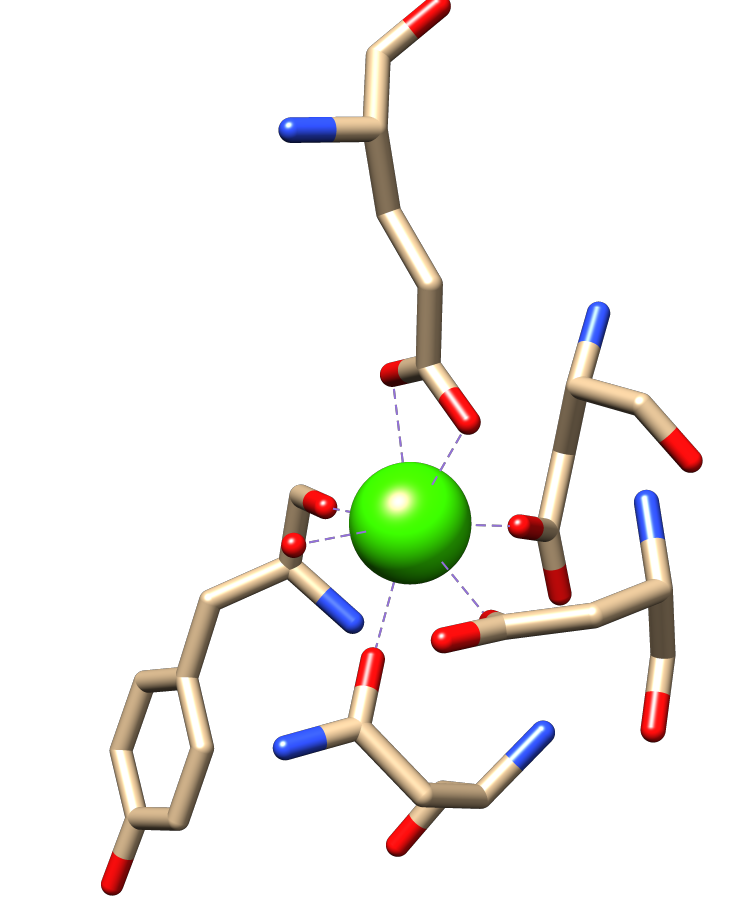
\includegraphics[width=0.49\textwidth]{rysunki/rozdzial_1/EFCaorientation2.png}%
	\label{fig:EFhandLeft}%
	}
\centering
	\subfloat[Heliksy E i F oraz pętla łącząca]{%
		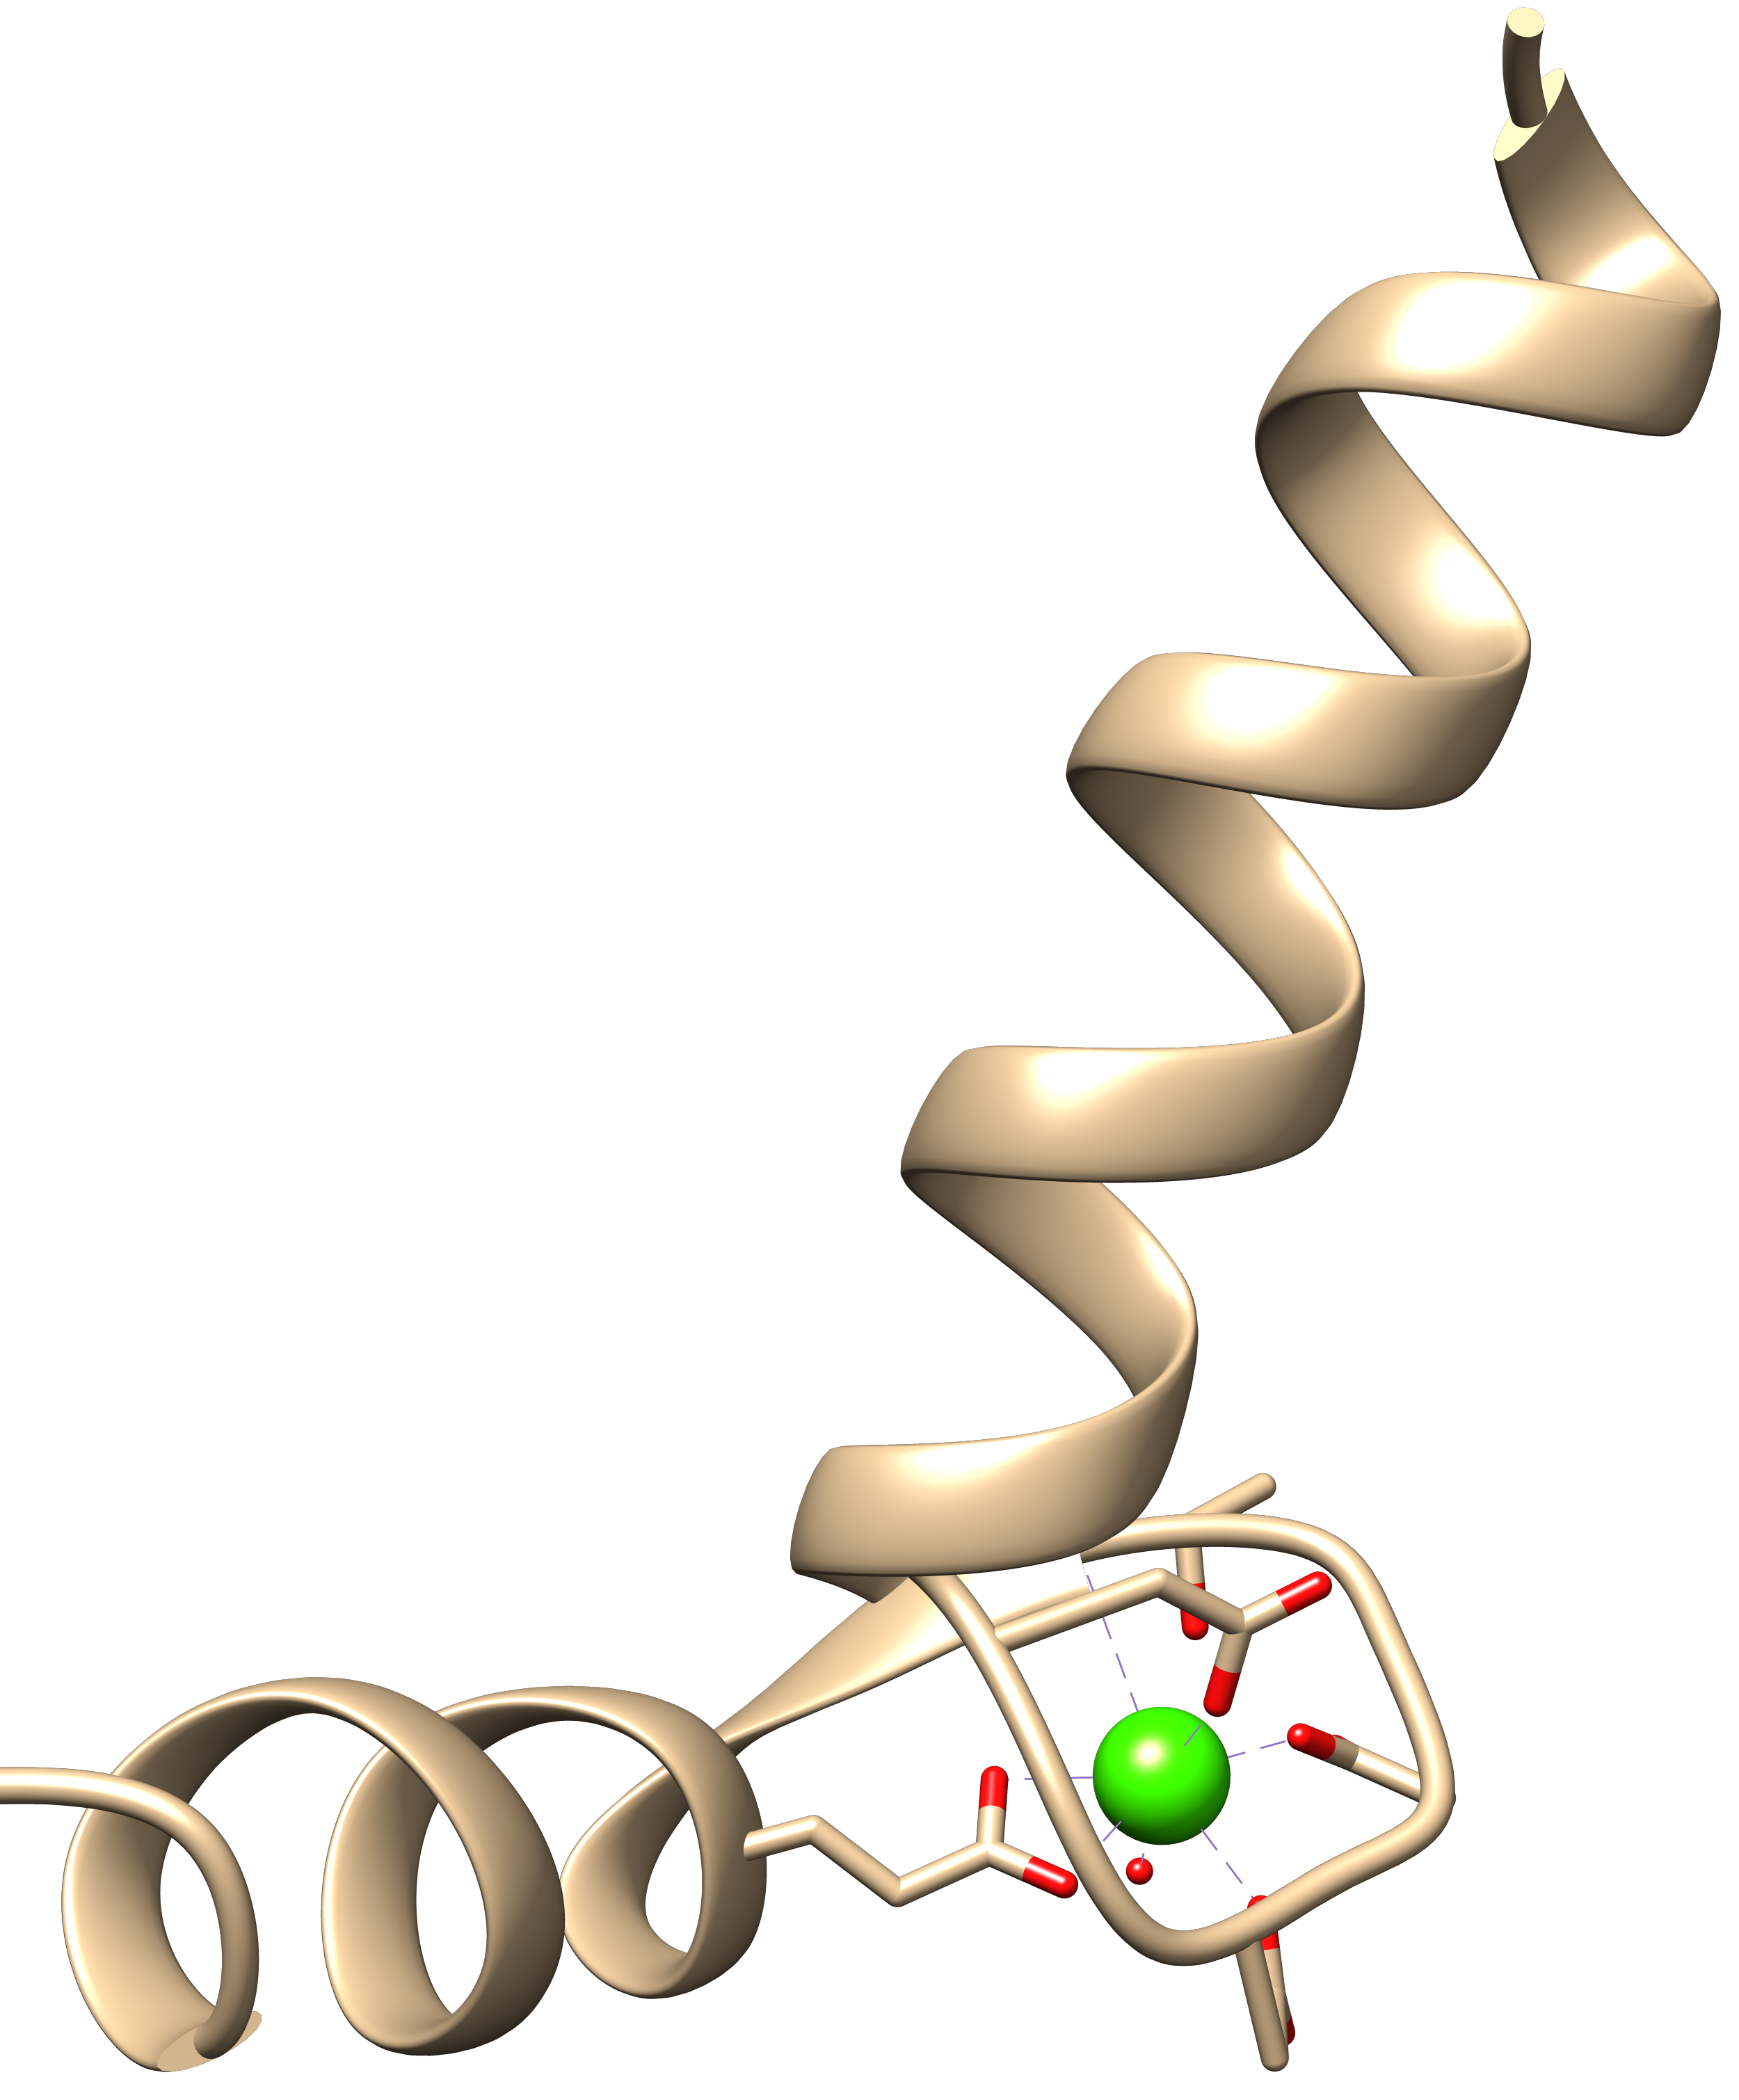
\includegraphics[width=0.49\textwidth]{rysunki/rozdzial_1/EF-hand-Ca.png}%
	\label{fig:EFhandRight}%
	}
\caption [Struktura motywu EF-hand]{Struktura motywu EF-hand.}
\label{fig:EFhand}
\end{figure}

\begin{figure}[tb]
	\centering
	\subfloat[kalmodulina, bez Ca$^{2+}$ (kod PDB: \textbf{1CFD})]{%
		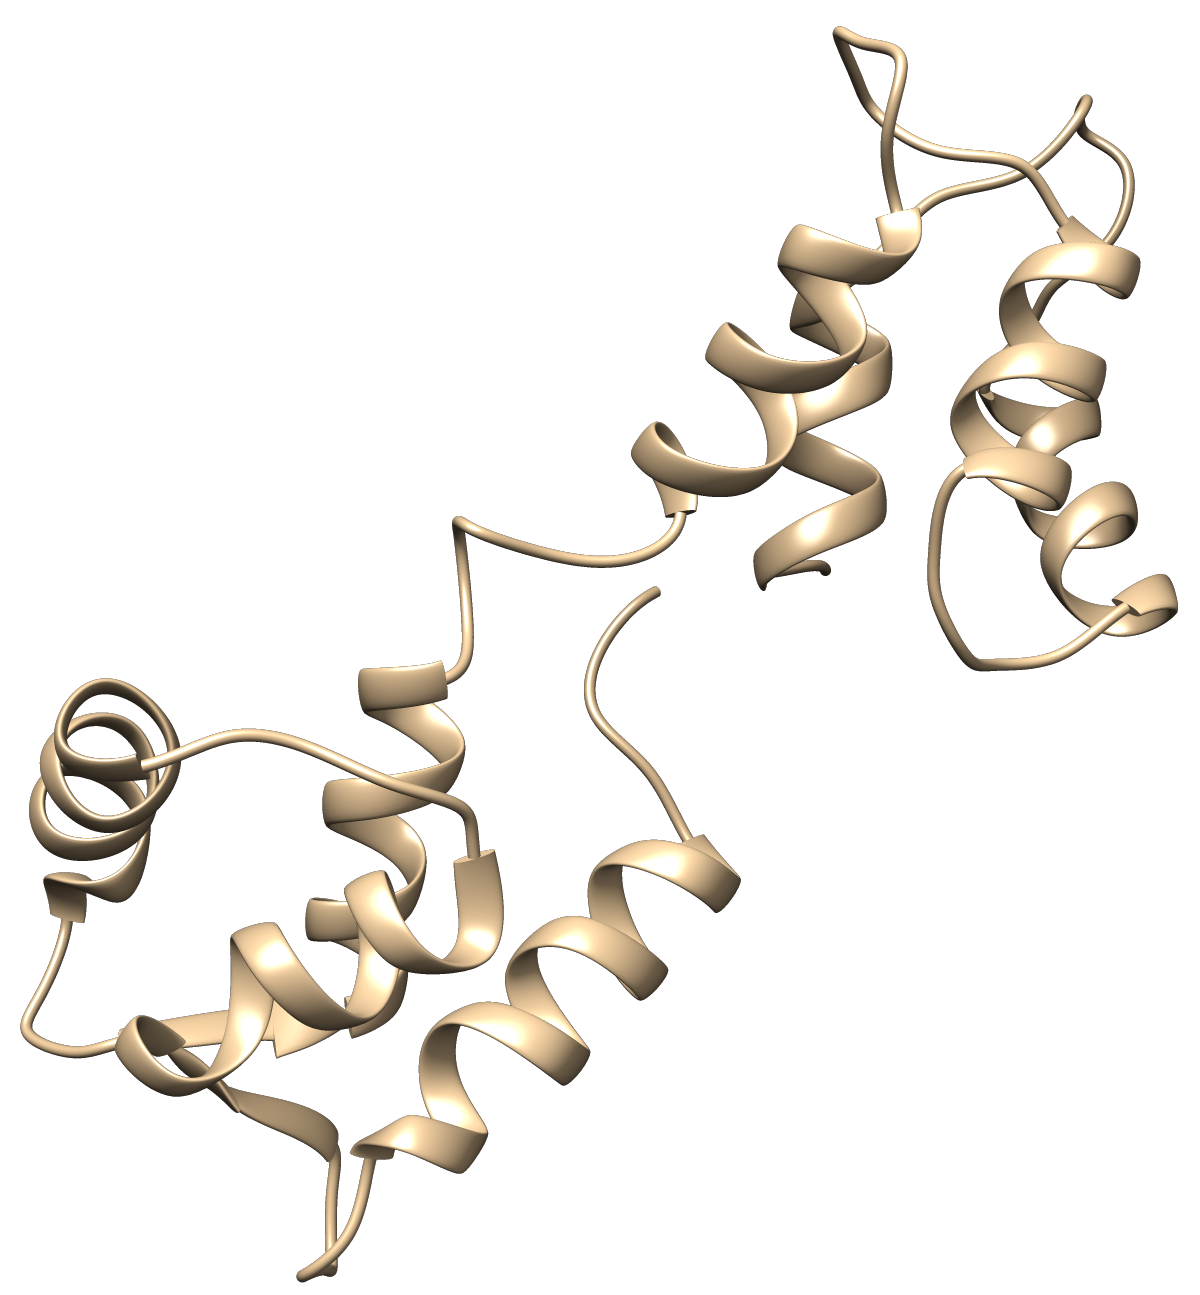
\includegraphics[width=0.48\textwidth]{rysunki/rozdzial_1/camapo.png}%
		\label{fig:camleft}%
	}
	\centering
	\subfloat[kalmodulina z Ca$^{2+}$ (kod PDB: \textbf{3CLN})]{%
		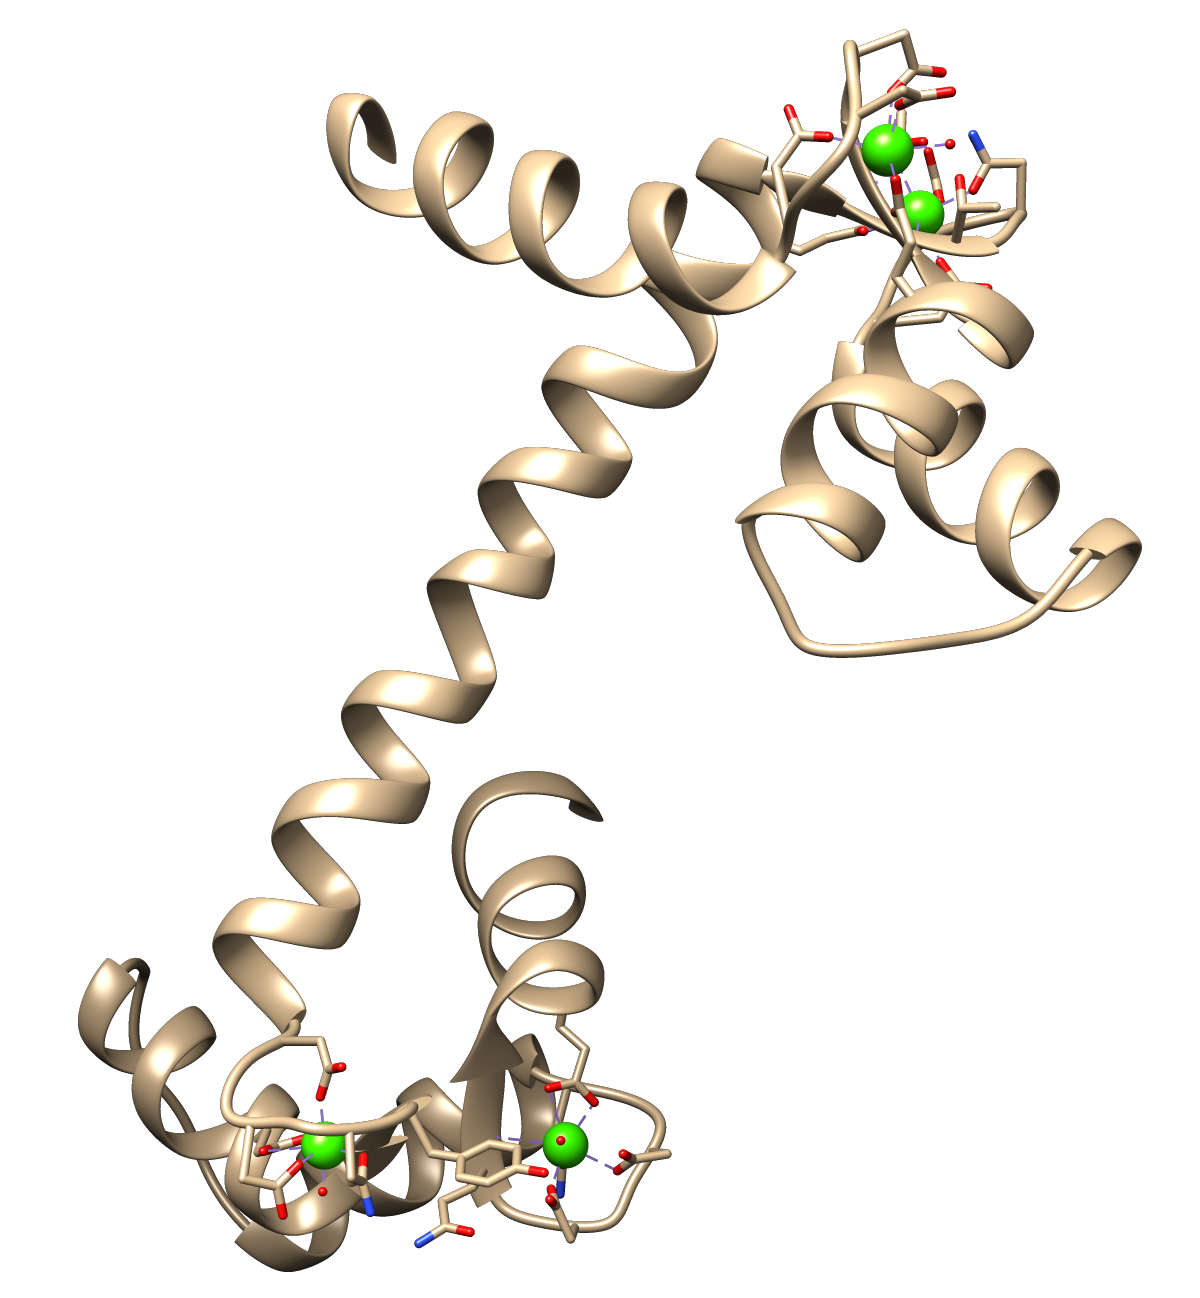
\includegraphics[width=0.48\textwidth]{rysunki/rozdzial_1/camca.png}%
		\label{fig:camright}%
	}
	\caption[Struktura kalmoduliny]{Wstążkowa reprezentacja struktury trzeciorzędowej kalmoduliny \cite{Babu1988,Kuboniwa1995}.}
	\label{fig:cam}
\end{figure}

Termin ''EF-hand'' wprowadzono w 1973 roku. Termin ten opisowo przedstawiał reprezentacje wstążkową domeny odpowiedzialnej za wiązanie Ca$^{2+}$ w parvalbuminie. Białka EF-hand stanowią najważniejszą rodzinę białek wiążących wapń (tzw. \textit{,,EF-hand calcium binding proteins''}). Jest to bardzo różnorodna i liczna rodzina białek, której przedstawiciele zaliczaja sie z~reguły do sensorów Ca$^{2+}$ \cite{Yanez2012}. Klasycznym przykładem jest tutaj kalmodulina (CaM)\nomenclature{CaM}{kalmodulina} (Ryc.~\ref{fig:cam}). Motyw wiążący wapń składa się z~układu heliks-pętla-heliks, w którym wiązanie wapnia zachodzi właśnie w pętli łączącej helisy, złożonej zwykle z dwunastu aminokwasów~\ref{fig:EFhand}~\cite{Grabarek2006,Nelson2002}. Mechanizm wiązania opiera się na dwunastu negatywnie naładowanych atomach tlenu, z reszt hydroksylowych i~karbonylowych szkieletu białkowego heliksów i~podstawników grup bocznych, które oddziałują elektrostatycznie z~jonami wapnia. Z reguły w białku wiążącym wapń występują dwie takie pętle.

Jeżeli w białku występuje więcej motywów EF (nawet do 12), mamy do czynienia ze zjawiskiem kooperatywnego wiązania jonów wapnia. Związanie jednego jonu zwiększa powinowactwo kolejnych miejsc wiązania \cite{Lewit-Bentley2000}. Cząsteczka kalmoduliny zawiera dwie domeny z~motywem EF, co sprawia, że wiąże 4 jony wapnia. Stała dysocjacji takiego układu wynosi $K_d \sim 10^{-6}$ M. Po związaniu Ca$^{2+}$ kalmodulina zmienia konformację, eksponując domeny hydrofobowe. Kalmodulina reguluje funkcję~i~aktywność około 300 białek, m.in.: kalcyneuryny, syntazy tlenku azotu (NOS - ang. \textit{\textbf{n}itric \textbf{o}xide \textbf{s}ynthase})\nomenclature{NOS}{syntaza tlenku azotu (ang. \textit{\textbf{n}itric \textbf{o}xide \textbf{s}ynthase})}, receptora IP$_3$R, PMCA \cite{Stull2001}.
Liczba białek posiadających ten motyw jest olbrzymia. Szacuje się, że jest ich od 600 do kilku tysięcy. Ogólnie można podzielić je na 66 dużych rodzin, liczących sobie kilku, bądź kilkuset przedstawicieli. Pod względem funkcjonalnym zgrupowanych w~dwie duże podgrupy (Ryc.~\ref{fig:EFhandtree}) \cite{Zhou2006}:

\begin{bulletList}
\item \textbf{Kanoniczne EF-hand} - występujące np. w kalmodulinie (Ryc.~\ref{fig:EFhand}), gdzie 12 reszt pętli stabilizuje jon wapnia poprzez tlen reszt karboksylowych.
\item \textbf{Pseudo EF-hand} - znajdujące się np. w białkach S100, które posiadają zmodyfikowaną sekwencję pętli aminokwasowej wiążącej wapń.
\end{bulletList}

\begin{figure}
	\centering
	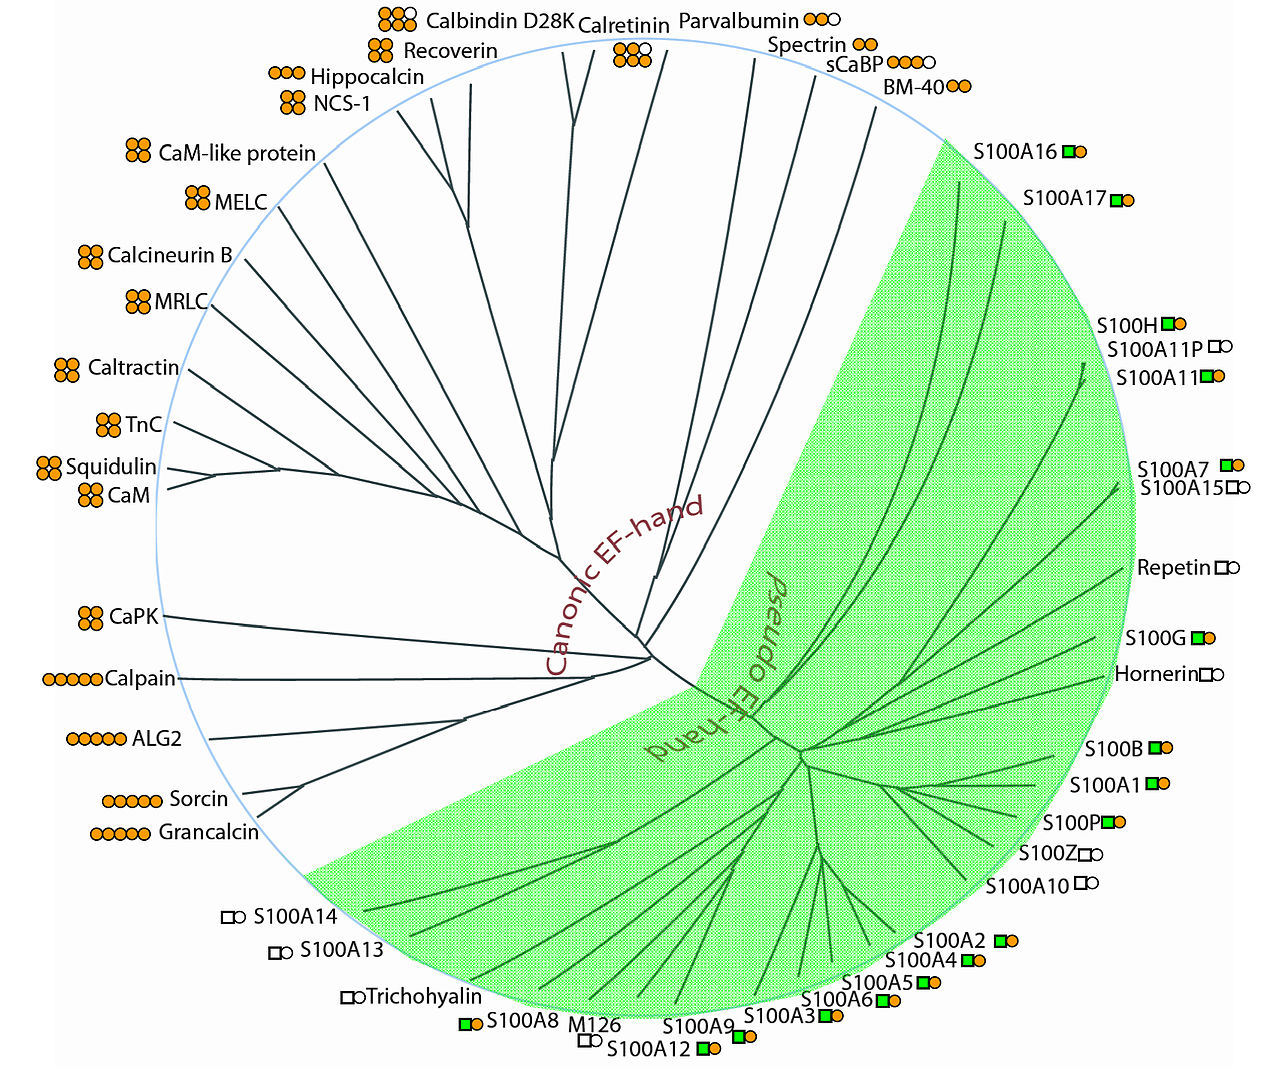
\includegraphics[width=0.85\textwidth]{rysunki/rozdzial_1/EFhandtree.jpg}
	\caption[Drzewo filogenetyczne białek z rodziny EF-hand]{Drzewo filogenetyczne białek z rodziny EF-hand \cite{Zhou2006}.}
	\label{fig:EFhandtree}
\end{figure}


\FloatBarrier
\subsubsection{Motywy C2}

Domena C2 liczy $\sim$120 aminokwasów o silnie konserwowanej sekwencji (Ryc.~\ref{fig:C2}). To charakterystyczny motyw złożony z ośmiu anty-równoległych $\beta$-kartek, jedna na drugiej. Tego typu układy zdolne są wiązać od dwóch do trzech jonów wapnia. Wiązanie następuje w pętlach utworzonych z~wolnych łańcuchów aminokwasów występujących pomiędzy $\beta$-kartkami. Występują z~reguły w białkach, które wykorzystują ładunek Ca$^{2+}$ do przemieszczenia się w pobliże dwuwarstwy lipidowej, np. fosfolipaza C, synaptotagmina, białkowa kinaza C \cite{Nalefski1996,Traore2013}.

\begin{figure}[h]
\vspace{-10pt}
\centering
	\subfloat[C2 bez Ca$^{2+}$ (kod PDB: \textbf{3W56})]{%
		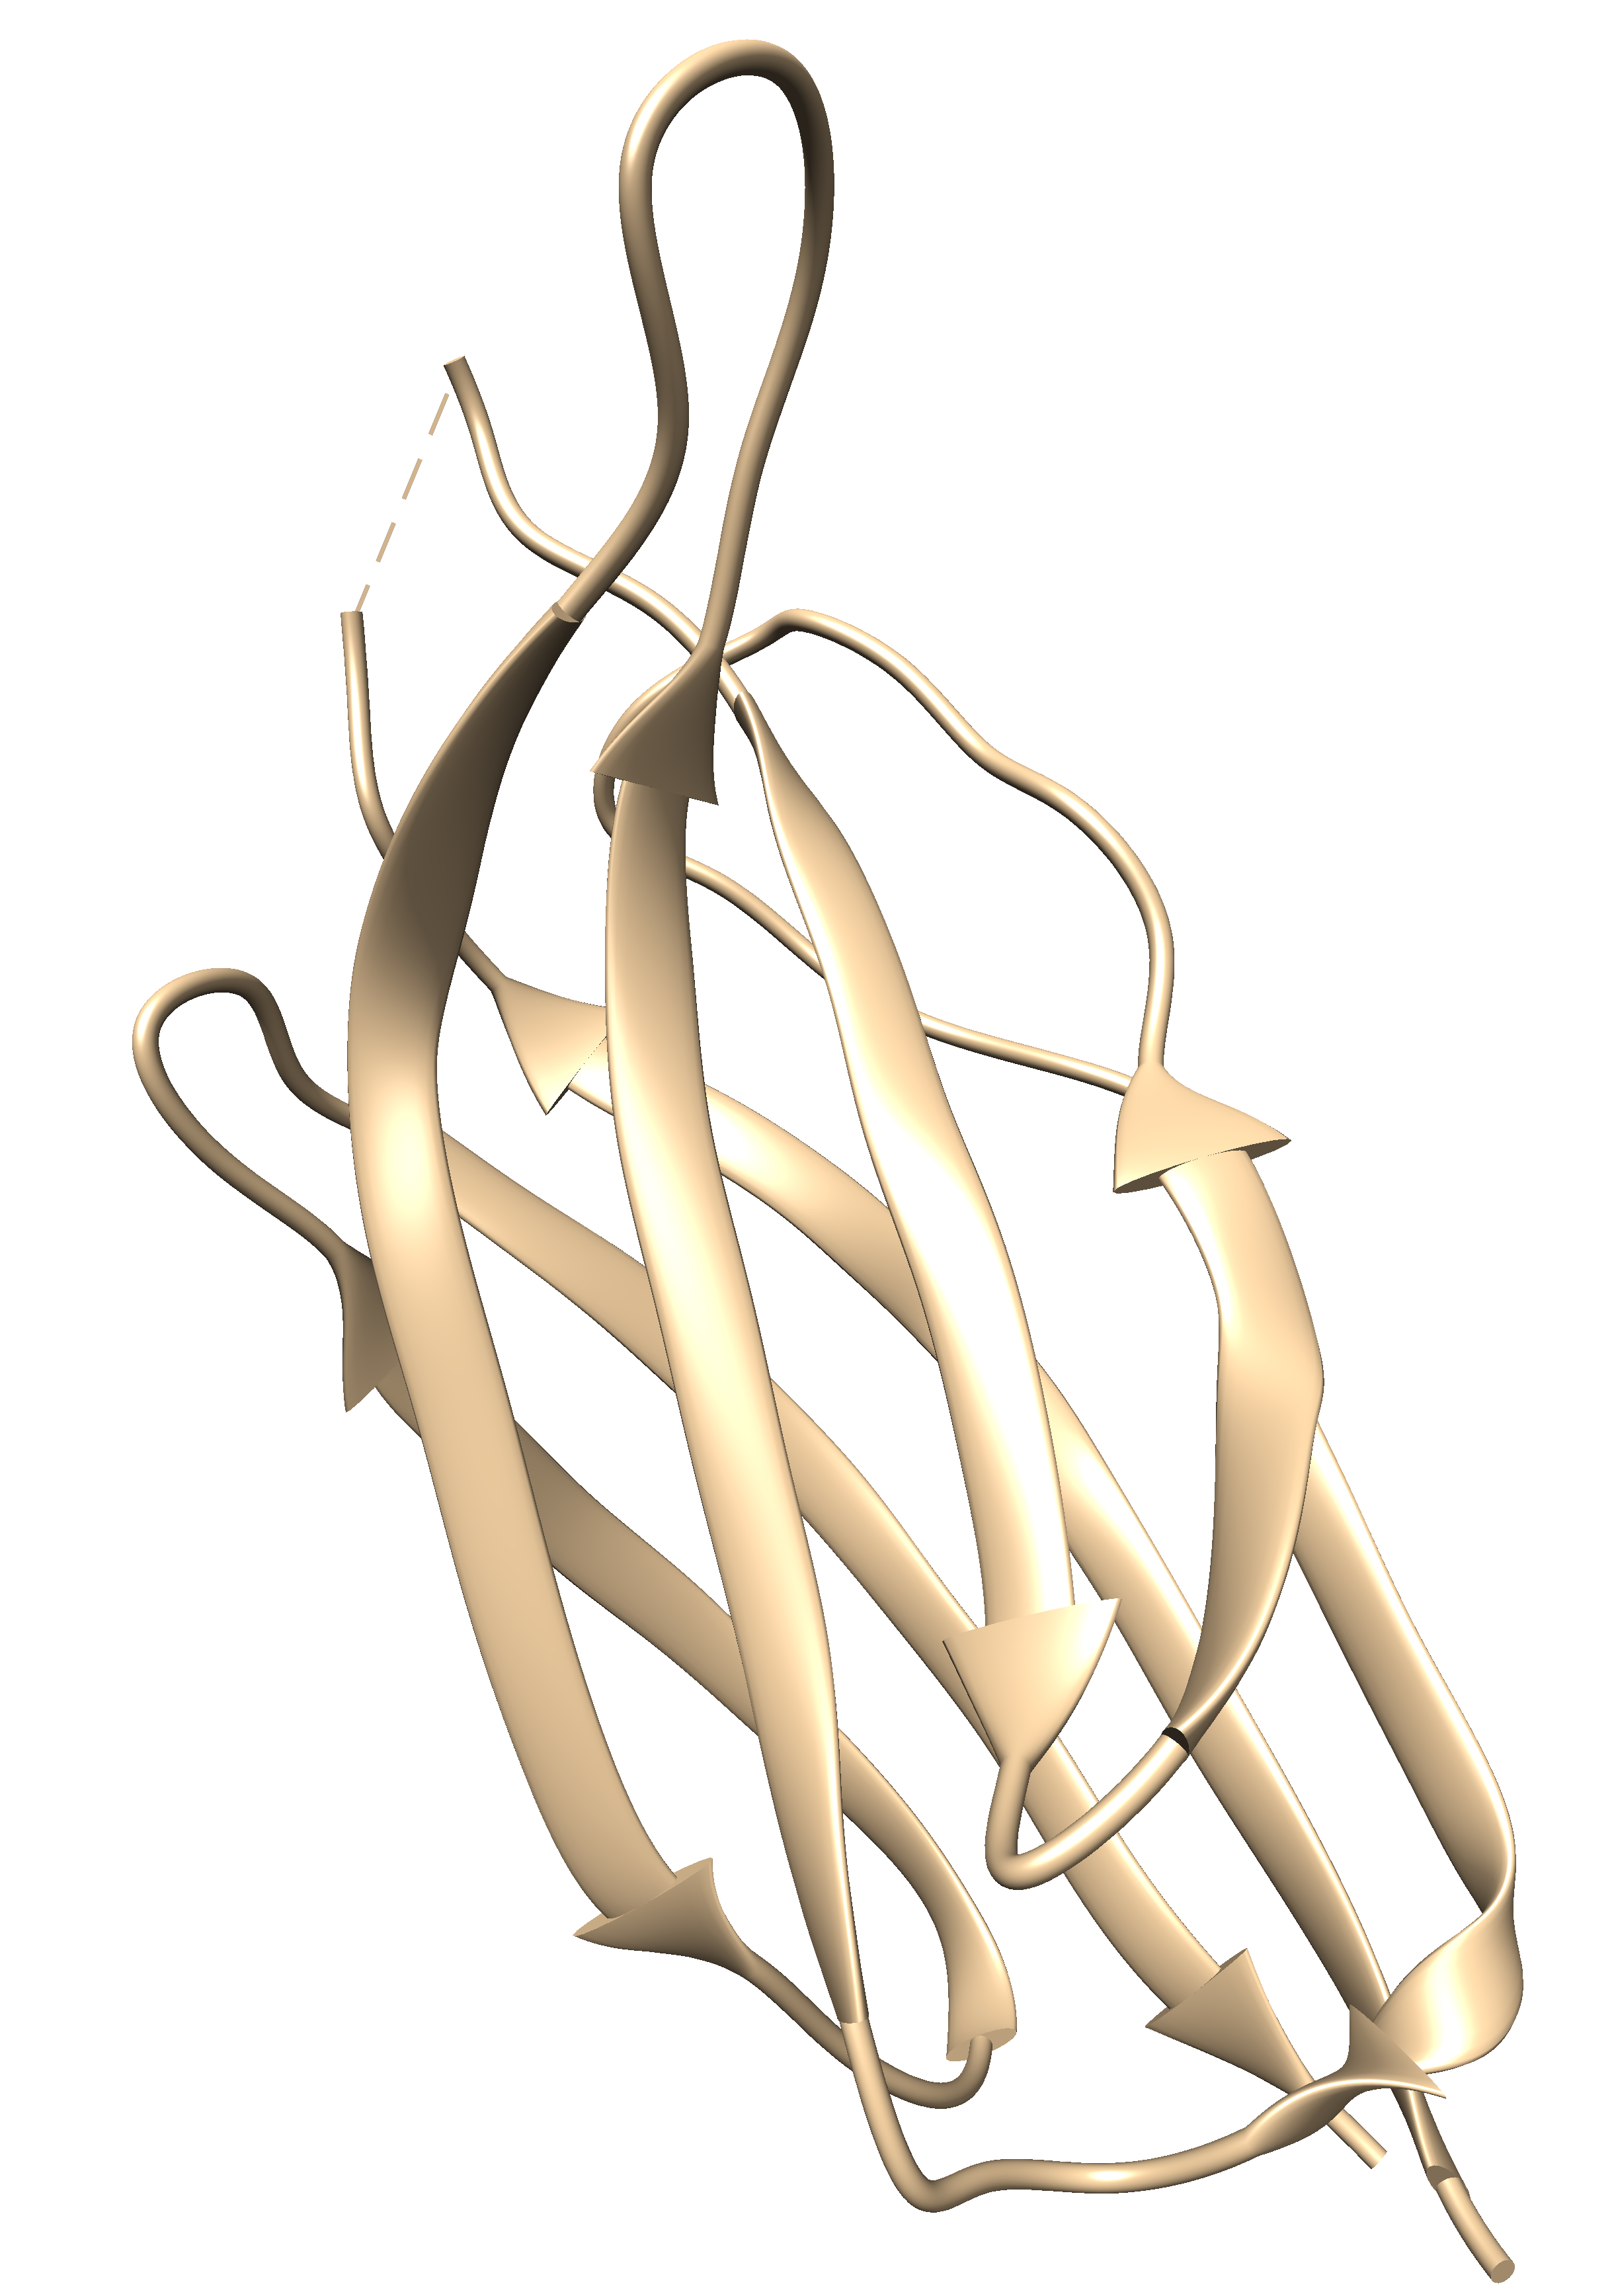
\includegraphics[width=0.5\textwidth]{rysunki/rozdzial_1/C2apo.png}%
	\label{fig:c2left}%
	}
\centering
	\subfloat[C2 z Ca$^{2+}$ (kod PDB: \textbf{3W57})]{%
		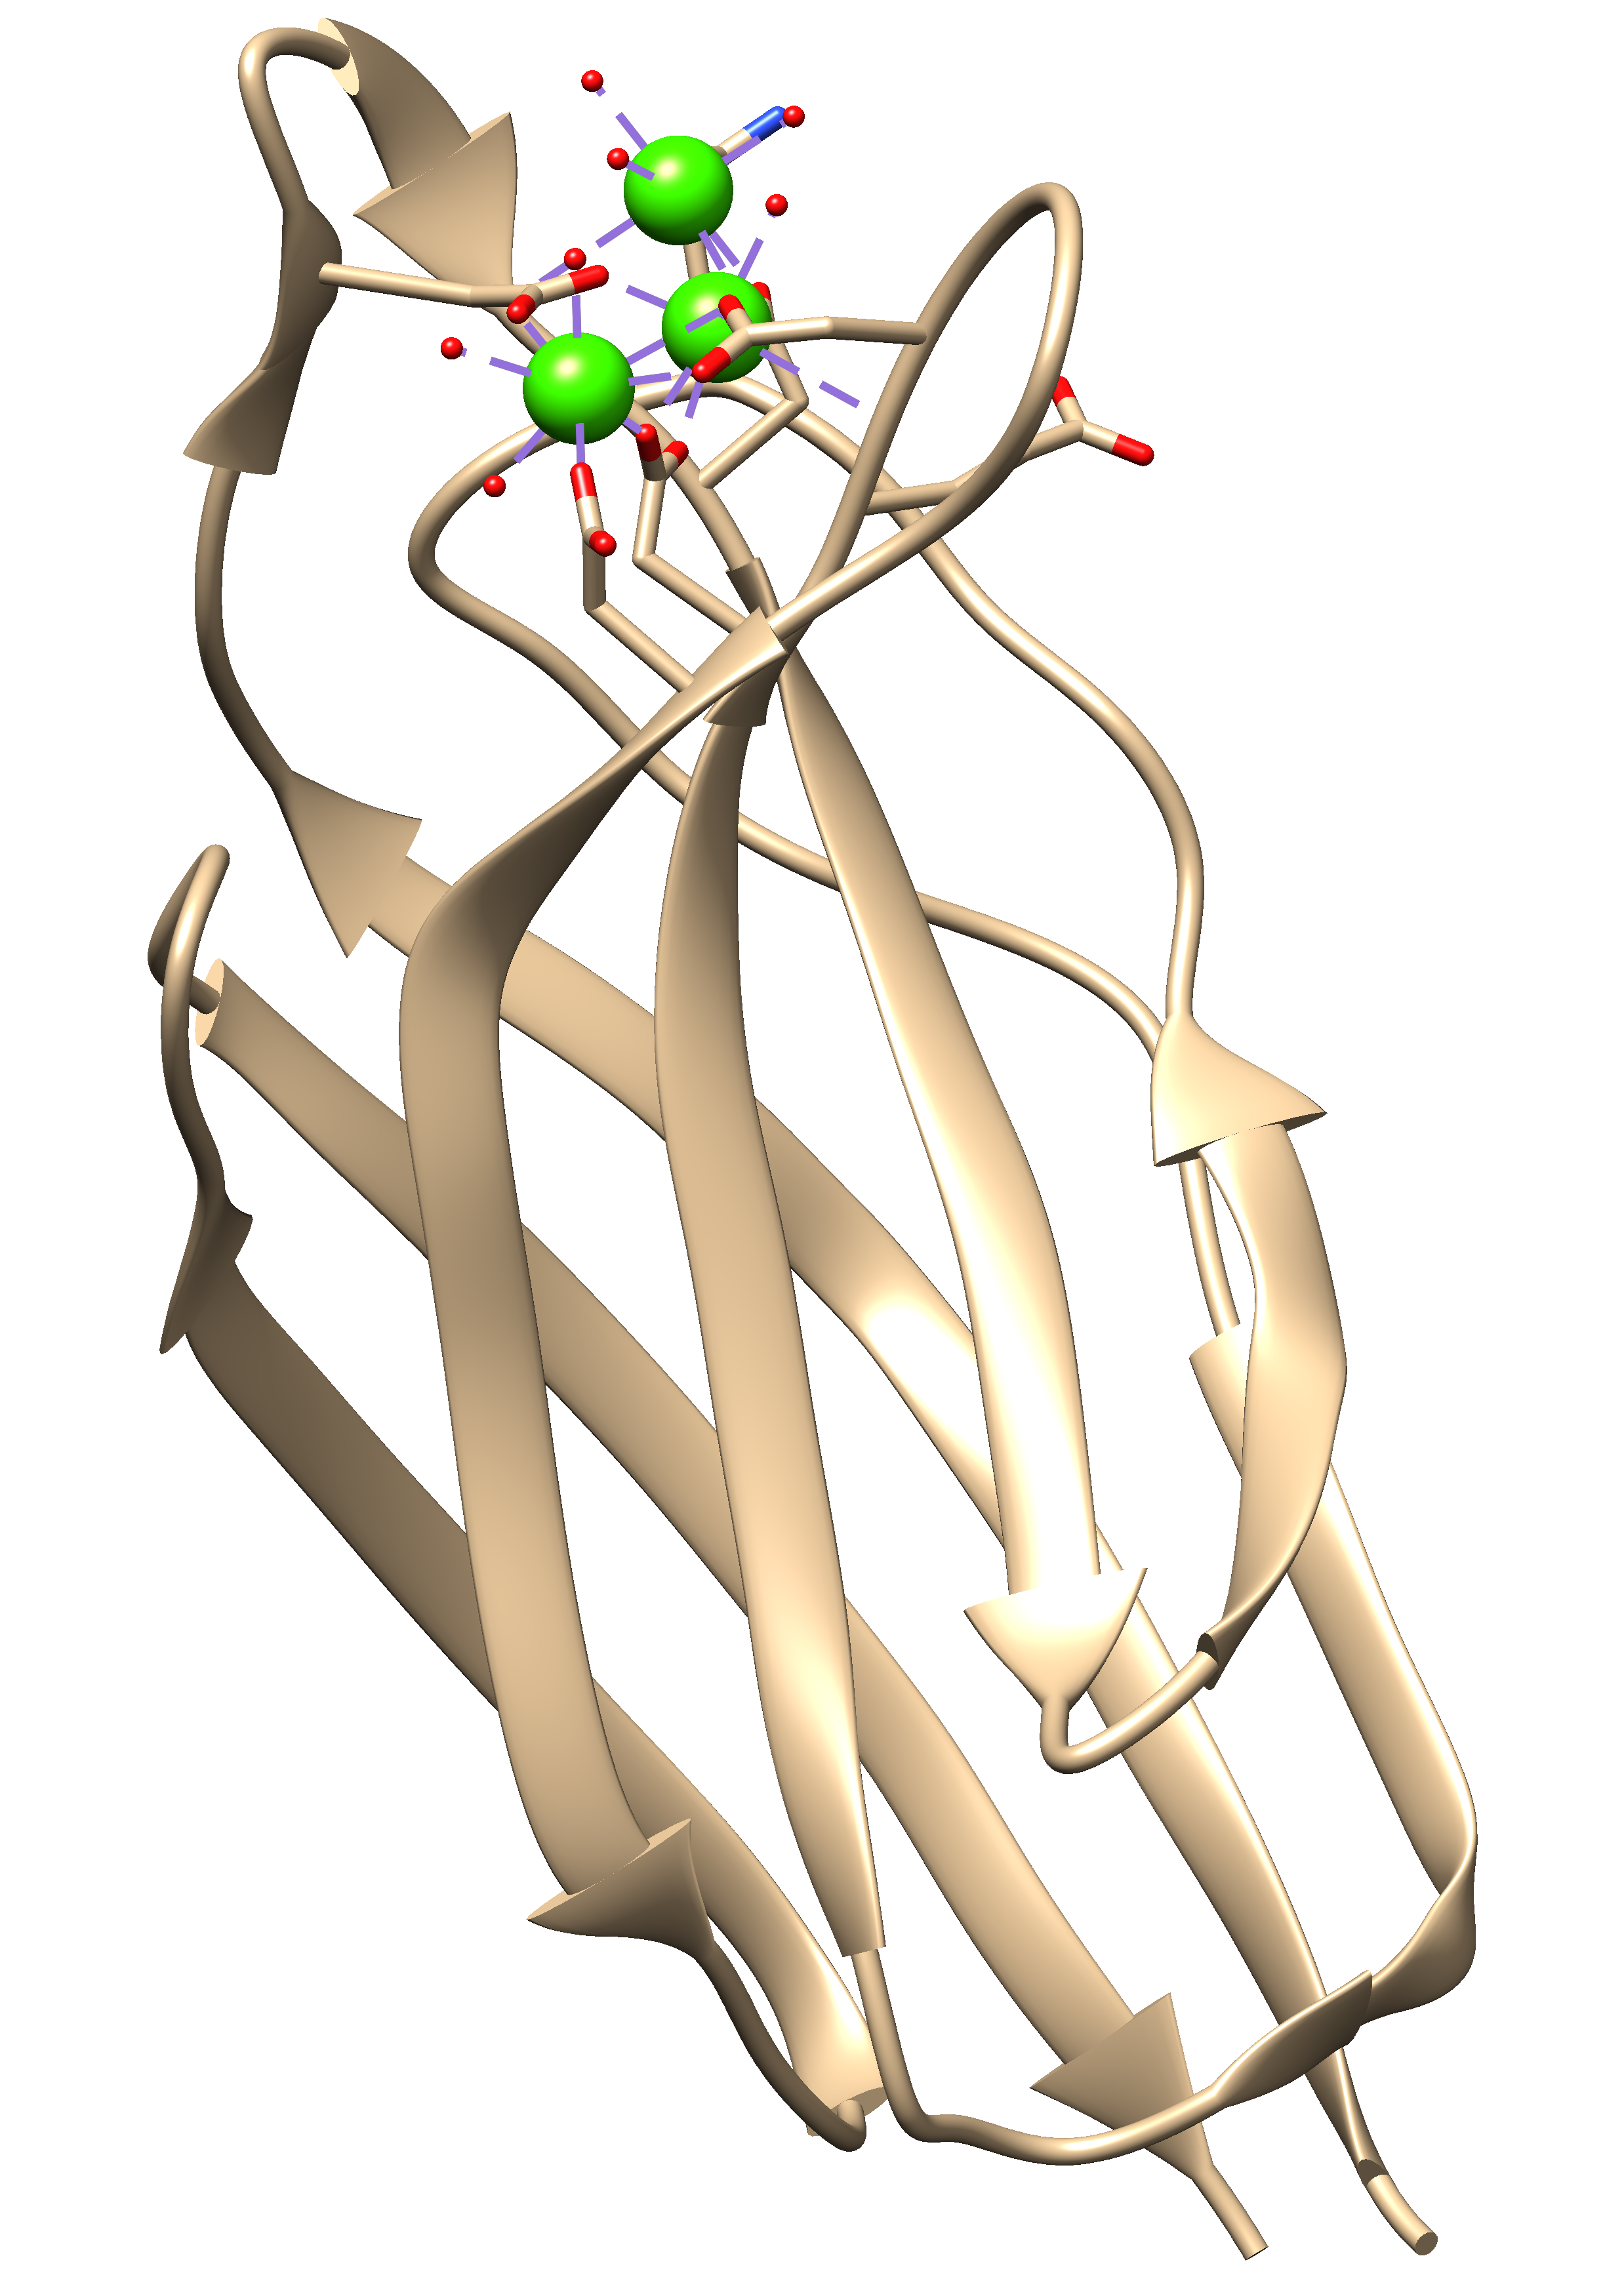
\includegraphics[width=0.5\textwidth]{rysunki/rozdzial_1/C2Ca.png}%
	\label{fig:c2right}%
	}
\caption[Motyw C2]{Wstążkowa reprezentacja struktury trzeciorzędowej motywu C2 \cite{Traore2013}.}
 \label{fig:C2}
\end{figure}

Kilka jonów potrafi wytworzyć pole elektrostatyczne, pozwalające znacznie przyśpieszyć wiązanie z białkami na powierzchni błony komórkowej (np. w przypadku fosfolipazy, która wykorzystuje domenę C2 do zbliżenia się do inozytolu na powierzchni błony). Związanie Ca$^{2+}$ w~pętlach obniża negatywny ładunek białka i pozwala na penetrację dwuwarstwy lipidowej przez reszty hydrofobowe i aromatyczne.

%\FloatBarrier
\subsection{Przepływy wapnia z i do komórki}

Poziom jonów wapnia w komórce podlega ścisłej regulacji. Stężenie tych jonów w~środowisku zewnątrzkomórkowych wynosi w przybliżeniu $\sim$~2mM, z kolei w cytozolu, podczas spoczynku jest stosunkowo niskie i wynosi 20 -- 100 nM w zależności od rodzaju komórki. Tak niski poziom wapnia jest konieczny ze względu na obecność fosforanów, których sole z wapniem są słabo rozpuszczalne, więc dochodziłoby do precypitacji i~utraty tych ważnych dla komórki związków. Duży gradient stężenia Ca$^{2+}$ występuje także pomiędzy cytozolem, a~siateczką śródplazmatyczną. Stężenie Ca$^{2+}$ w~ER jest ok. 1000 razy większe niż w cytoplazmie i wynosi $\sim$0.5 -- 1 mM. Stężenie wapnia w mitochondrium waha się pomiędzy 50 -- 500$\mu$M (Ryc.~\ref{fig:toolkit}) \cite{Clapham2007}. Szereg wyspecjalizowanych białek (Rozdz.~\ref{bialkaTransportowe}) zaangażowanych jest w utrzymaniu ,,status quo'', czyli niskiego poziomu wapnia w cytozolu. Tworzą układ pomp, kanałów i wymienników, które kontrolują stężenie Ca$^{2+}$ w cytozolu, utrzymując jego poziom w stanie równowagi dynamicznej. Sygnał wapniowy tworzą poszczególne przepływy: napływ jonów wapnia ze środowiska zewnątrzkomórkowego do wnętrza komórki oraz wypływ, uwalnianie z~magazynów wewnątrzkomórkowych i transport w przeciwnym kierunku.

Wapń do większości typów komórek napływa głównie poprzez \textbf{kanały bramkowane napięciem} (VGCC) \cite{Zamponi2005} lub \textbf{ligandem} (LGCC) \cite{Whitfield2001}, znajdujące się na błonie komórkowej. Istnieje jednak szereg innych mechanizmów napływu jonów wapnia, które wykorzystują wyspecjalizowane białka/kanały np.: kanały wapniowe zależne od receptorów (ROCC) \cite{Schwaller2012}, kanały pojemnościowego napływu wapnia (SOCEC) \cite{Parekh2005}, kanały TRP \cite{Pedersen2005}.


\begin{table}[h]
\centering
\begin{tabular}{p{2.7cm}p{4.55cm}p{7cm}}
\toprule[0.12em]
\textbf{Typ kanału}& \textbf{Miejsce} & \textbf{Opis} \\
& \textbf{występowania} & \\\midrule[0.06em]
%\multicolumn{3}{>{\columncolor[gray]{.9}}l}{\rule[-2ex]{0pt}{5.5ex}\textbf{Bramkowane napięciem}}\\[0.12em]
\rule[-2ex]{0pt}{5.5ex} \textbf{Typ L}\newline(Ca$_V$ 1.1-1.4) & komórki mięśniowe oraz inne komórki zwierzęce & aktywacja przy wysokim potencjale błony,regulacja skurczu komórek mięśniowych \\[1.2em]
\textbf{Typ N}\newline(Ca$_V$ 2.2) & neurony & aktywacja przy wysokim potencjale błony; wolniejsza inaktywacja niż kanały T; sekrecja neurotransmitterów \\[1.2em]
\textbf{Typ P}\newline(Ca$_V$ 2.1) & neurony gruszkowate (Purkinjego) inne kom. nerwowe & napięcie, fosforylacja, białka G; uwalnianie neurotransmitterów w szczelinach presynaptycznych, również znajdowane we włóknach Purkinjego serca.\\[1.2em]
\textbf{Typ Q}\newline(Ca$_V$ 2.1) \newline & komórki ziarniste móżdżka & wysoki poziom aktywacji i relatywnie niska kinetyka. \\[1.2em]
\textbf{Typ R} \newline(Ca$_V$ 2.3) & komórki ziarniste móżdżka & wysoki poziom aktywacji i relatywnie niska kinetyka działania. \\[1em]
\textbf{Typ T}\newline(Ca$_V$ 3.1-3.3) & powszechnie w~komórkach zwierzęcych & aktywacja przy niskim potencjale błony, regulacja wejścia wapnia przy ujemnym
potencjale błony \\[1em]
%\multicolumn{3}{>{\columncolor[gray]{.9}}l}{\rule[-2ex]{0pt}{5.5ex} \textbf{Bramkowane ligandem}}\\[.12em]
%\rule[-2ex]{0pt}{5.5ex} \textbf{IP$_3$}& w móżdżku i gładkich komórkach mięśniowych, także w trzustce, jelicie grubym i nerkach & Uwalnia jony wapnia z retikulum endoplazmatycznego\\[1.6em]
%\rule[-2ex]{0pt}{5.5ex} \textbf{RyR} & mięśnie szkieletowe, kardiomiocyty & Jest głównym czynnikiem odpowiedzialnym za mechanizm CICR \\[1.2em]
%\textbf{Uniporter} & wszystkie komórki zwierzęce & Odpowiedzialny głównie z a transport jonów wapnia do macierzy mitochondrium\\
\bottomrule[0.12em]
\end{tabular}
\caption [Kanały bramkowane napięciem]{Lista ważniejszych kanałów wapniowych, bramkowanym napięciem, występujących w komórkach eukariotycznych \cite{Fill2002,McDonough2004,Simms2014,Yoshida1997}.}
\label{tab:vgcc}
\end{table}





\FloatBarrier
\subsubsection{Kanały bramkowane napięciem (VGCC)}\label{ss:vgcc}

Kanały \textbf{VGCC}, które określane są również jako\textbf{ Ca$_V$}, występują w dużych ilościach w błonach komórek pobudliwych i stanowią niezbędny element prawidłowego funkcjonowania neuronów, gleju, mięśni szkieletowych, serca czy gruczołów wewnątrzwydzielniczych. Z reguły nie działają jako osobne kanały, lecz kooperują ściśle z innymi rodzajami kanałów jonowych - potasowymi i sodowymi lub kanałami aktywowanymi neuotransmiterami, wspierając potencjał czynnościowy (w neuronach) lub stanowiąc główną jego część (mięśnie serca). Ich otwarcie następuje w wyniku zmiany potencjału błonowego w stosunku do potencjału spoczynkowego komórki (-70 mV). VGCCs składane są z kilku podjednostek, które tworzą heteromultimery (najczęściej występujący kanał typu L składa się z się z pięciu podjednostek). Rdzeń kanału stanowi podjednostka $\alpha_1$ złożoną z czterech domen formujących pierścień w błonie białkowo-lipidowej o wielkości 170-250 kDa. Każda z domen zawiera 6 transbłonowych motywów o strukturze $\alpha$-helisy (Ryc.~\ref{fig:vgcc}). Co czwarty heliks posiada pozytywnie naładowane krótkie sekwencje transbłonowe o właściwości czujnika jonów Ca$^{2+}$. Już pojedynczy pierścień ma funkcjonalność kanału jonowego, ale z reguły podjednostka $\alpha$ sprzężona jest dodatkowo z innymi podjednostkami (np. $\alpha_2$, $\beta$, $\gamma$, $\delta$), które modyfikują kinetykę aktywacji/dezaktywacji i lokalizację kanału (Tab.~\ref{tab:vgcc}) \cite{Tang2014,Yamakage2002}.

\begin{figure}[h]
\centering
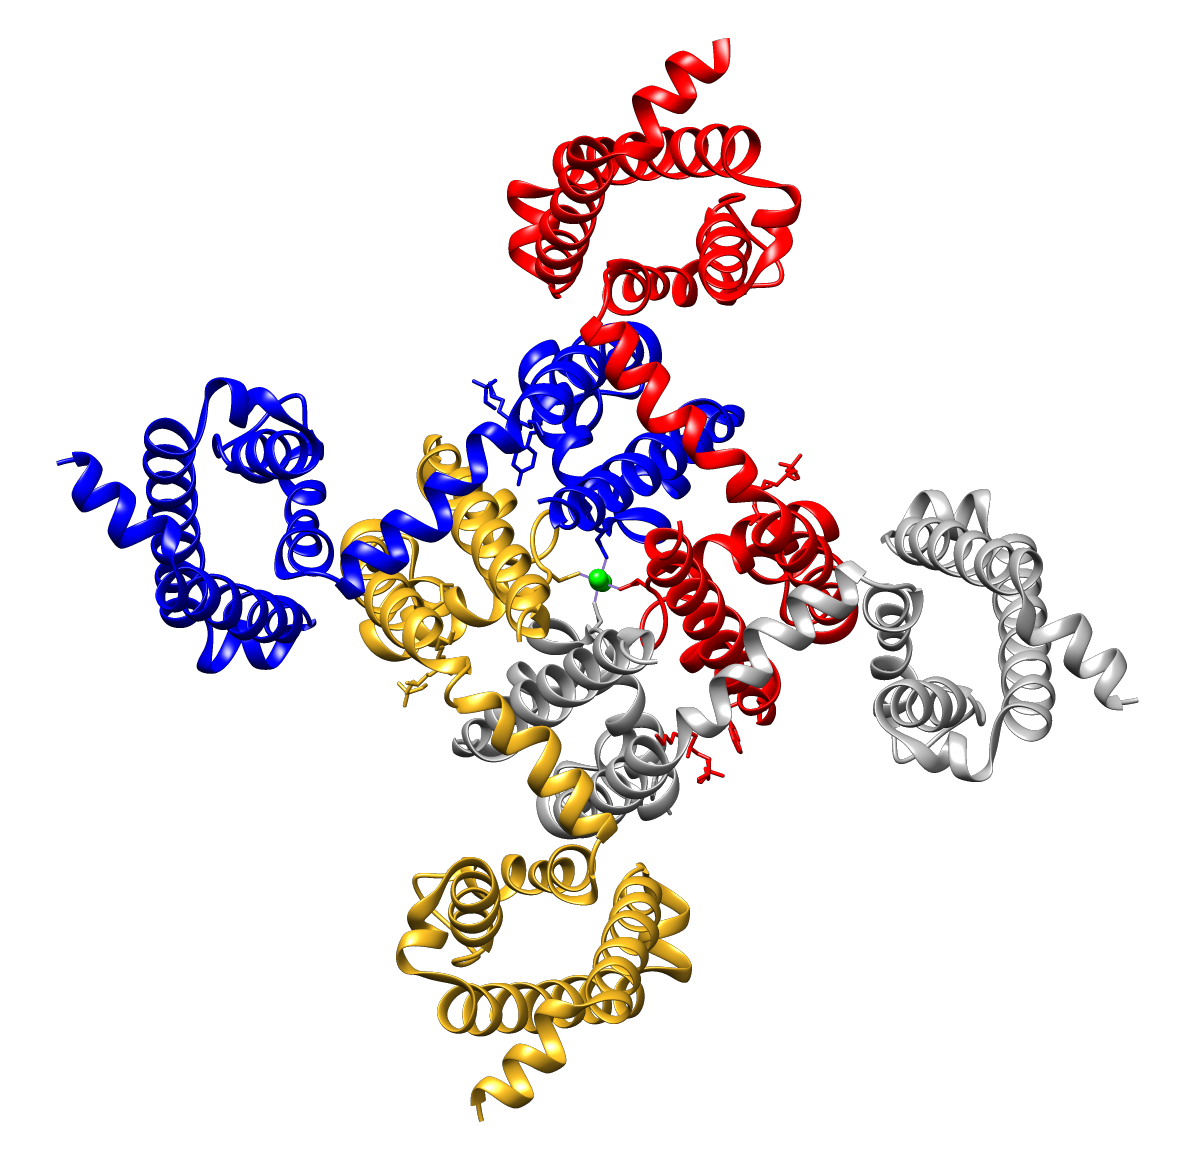
\includegraphics[width=0.5\textwidth]{rysunki/rozdzial_1/vgcc.png}%
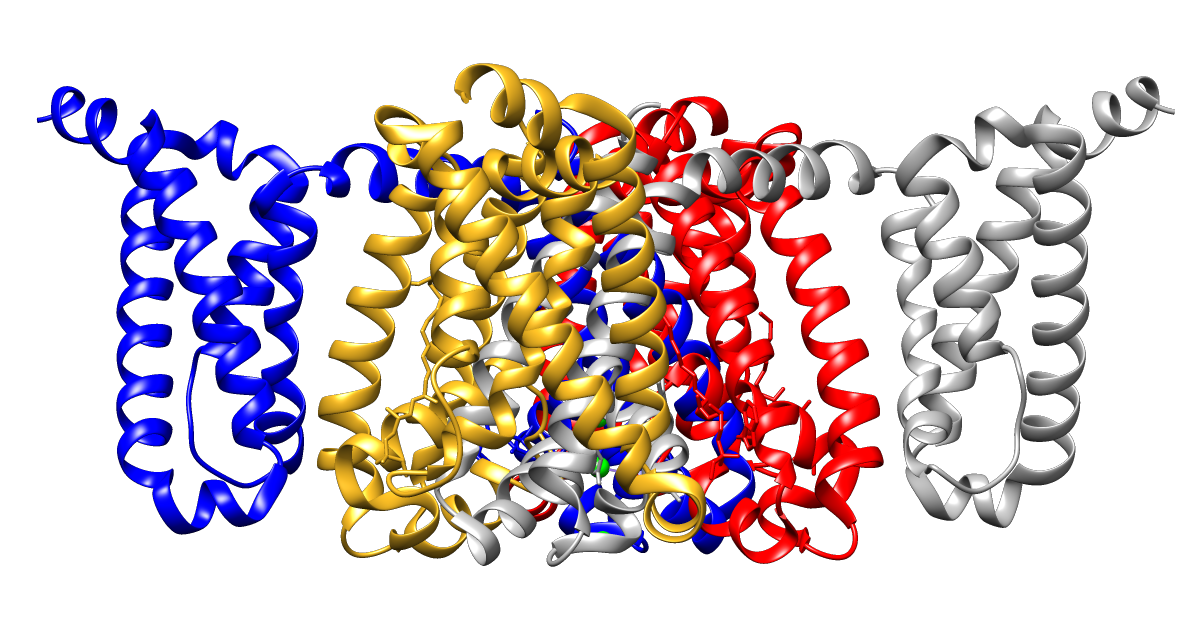
\includegraphics[width=0.5\textwidth]{rysunki/rozdzial_1/vgcc2.png}%
\caption [Struktura kanału VGCC]{Struktura czwartorzędowa kanału bramkowanego napięciem (kod PDB: \textbf{4MW3}). Kolorami oznaczono poszczególne łańcuchy tetrameru \cite{Tang2014}.}
\label{fig:vgcc}
\end{figure}

\begin{landscape}
\begin{table}
	\normalsize
\centering
\begin{tabular}{lccccccr}\toprule[0.12em]
\rule[-2ex]{0pt}{5.5ex}\textbf{Typ kanału} & \textbf{Typ L} & \textbf{Typ N} & \textbf{Typ P} & \textbf{Typ Q} & \textbf{Typ R} & \textbf{Typ T} & Referencje \\
& \textbf{Ca$_V$ 1.1-1.4} & \textbf{Ca$_V$ 2.2} & \textbf{Ca$_V$ 2.1} & \textbf{Ca$_V$ 2.1} & \textbf{Ca$_V$ 2.3} & \textbf{Ca$_V$ 3.1-3.3} & \\\midrule[0.06em]
Przewodność [pS]          & 25 & 11--20 & 9--20  & 15--16 & 15--20 &      8      & \cite{Sharman2013} \\
Selektywność (Ca$^{2+}$>Ba$^{2+}$) & 2:1     & 2:1   & 2:1  & --   & 1.3:1   & 1:1    & \cite{Sharman2013} \\
Potencjał aktywacji [mV]      & -10 -- -50 & -20   & -50  & -50  & -25 -- -40 & -70    & \cite{Sharman2013} \\
Czas deaktywacji [s]        & 0.15--2   & 0.1--0.2 & 0.5--1 & 0.5--1 & 0.05--0.1 & 0.01--0.07 & \cite{Sharman2013} \\\midrule[0.06em]
\textbf{Antagoniści (IC50) [$\mu$M]}& & &  &  & & &\\\midrule[0.06em]
$\omega$-konotoksyna MVIIA & brak & 0.078--1  & brak & brak & brak & brak & \cite{Pringos2011,Sharman2013} \\
$\omega$-konotoksyna GVIA  & brak & 0.028--2  & brak & brak & brak & brak & \cite{Pringos2011,Sharman2013} \\
$\omega$-agatoksyna AgaIVA & brak & brak    & 0.015 & 0.05--1 & 0.05 & brak & \cite{Pringos2011} \\
$\omega$-konotoksyna MVIIC & brak & 0.018   & 0.018 & 0.05--1 & brak & brak & \cite{McDonough1996,Pringos2011} \\
$\omega$-agatoksyna AgaIIIA & 0.001 & 0.001   & ND & ND & brak & brak & \cite{Ertel1994} \\
SNX-482           & brak    & brak & 0.03--0.75 & 0.03--0.75 & 0.015--0.03 & brak & \cite{Arroyo2003,Pringos2011} \\
Nimodypina         & 0.135--2.6 & brak & brak  & brak  & brak & 5--11  & \cite{Catterall2005,Furukawa2009,Stengel1998} \\
Nifedypina         & 0.1    & brak & brak  & brak  & brak & 39   & \cite{Stengel1998} \\
Efonidypina         & 10     & brak & brak  & brak  & brak & 1.3--13 & \cite{Furukawa2009,Masumiya2000} \\
Amplodypina         & 3--5    & brak & brak  & brak  & brak & 4--13  & \cite{Furukawa2009,Kwan1995} \\
Nikardypina         & 9--26   & brak & 32--97 & 32--97 & brak & 5--13  & \cite{Furukawa1999} \\
Verapamil          & 0.6--1   & brak & brak  & brak  & brak & 20--30 & \cite{Catterall2005,Freeze2006} \\
Diltiazem          & 3--33   & brak & brak  & brak  & brak & 30   & \cite{Catterall2005} \\
Mibefradil         & 1.7--21  & brak & 208  & 208  & brak & 0.5--11 & \cite{Aczel1998,Xi2001} \\\bottomrule[0.12em]
\end{tabular}
\caption [Podsumowanie właściwości VGCC]{Podział kanałów bramkowanych napięciem ze względu na wrażliwość na inhibitory i właściwości fizyko-chemiczne. \\Dane z IUPHAR-DB oraz \cite{Gurkoff2013,Simms2014}.}
\label{tab:vgccprop}
\end{table}
\end{landscape}

Istnieje kilka rodzajów VGCCs, które są strukturalnie homologiczne, lecz nie identyczne konstrukcyjnie. Wyszczególniono pięć podtypów kanałów VGCC, które różnią się właściwościami fizjologicznymi (np. czas otwarcia, przewodność i wrażliwość na potencjał) oraz wrażliwość na niektóre inhibitory. W zależności od tych różnic VGCCs dzielimy na kanały L, N, P, Q, R i T (Tab.~\ref{tab:vgcc}). Np. kanały typu L, są wrażliwe na zablokowanie przez 1,4-dihydropirydynę (DHP), ale nie przez $\omega$-konotoksynę, wyizolowana z jadu ślimaka \emph{Conus geographus} ($\omega$CTX) lub $\omega$-agatoksynę, wyizolowaną z jadu węży grzechotnikowatych ($\omega$AGA). Dane dotyczące pozostałych typów kanałów znajdują się w Tab.~\ref{tab:vgccprop} \cite{Gurkoff2013,Simms2014}.

Jak już wspomniano, kanały VGCCs aktywowane są zmianą potencjału elektrycznego na powierzchni błony komórkowej. Zmiana wpływa na układ sensorów jonów Ca$^{2+}$ w $\alpha$-helisach, dochodzi do zmiany konformacji i otwarcia kanału. Jony wapnia swobodnie przemieszczają się ze środowiska zewnątrzkomórkowego do cytozolu zgodnie z gradientem stężenia \cite{Lacinova2005}. Wapń wchodzący do komórki przez VGCC inicjuje dalsze etapy propagowania sygnału w komórce, poprzez aktywację mechanizmów efektorowych: kinaz białkowych, białek sensorowych i innych przekaźników drugiego rzędu.

Kanały te są wysoce selektywne, mimo to bardzo szybkie i mogą powodować lokalnie duży wzrost stężenia wapnia: >1 mM w~odległości $\sim$1$\mu$m od ujęcia wylotu kanału \cite{Piedras-Rentera2012}.

\subsubsection{Kanały bramkowane ligandem (LGCC)}\label{ss:lgcc}

Inną grupą kanałów, które uczestniczą w transporcie wapnia do wnętrza komórki jest grupa tzw. receptorów jonotropowych lub kanałów jonowych bramkowanych ligandem (LGCC). W wyniku wiązania ligandu z domeną receptorową, która znajduje się w miejscu allosterycznym białka z dala od samego kanału, receptor jonotropowy zmienia swoją konformację, w tym domen tworzących kanał jonowy. Kanał otwiera się umożliwiając napływ kationów (Ca$^{2+}$, K$^+$, Na$^+$) lub anionów (Cl$^-$), które przenikają przez błonę komórkową zgodnie z gradientem stężeń. Ze względu na specyficzny charakter wiązania receptora do ligandu, kanały te dzielimy właśnie według cząsteczki transmitera, który go aktywuje. Są to: acetylocholina (Ach), serotonina (5-HT), kwas $\gamma$-aminomasłowy (GABA), kwas glutaminowy oraz nukleotydy purynowe (np. ATP). Większość z wymienionych typów receptorów może transportować jony wapnia, jedynie receptopry GABA sprzężone są z kanałami transportującymi jony chlorkowe, zostaną więc pominięte w dalszym opisie.

Pod względem strukturalnym wyróżnić możemy trzy kategorie receptorów jonotropowych, w których kanał jonowy tworzony jest przez pięć, cztery i trzy podjednostki. Do jednej z rodzin należą tzw. receptory o budowie \textbf{pentamerycznej}, do której należą nikotynowe receptory cholinergiczne (nAChR - ang. \textit{\textbf{n}icotinic \textbf{a}cetyl\textbf{ch}oline \textbf{r}eceptors}) \cite{Beker2003,Weber2005}\nomenclature{nAChR}{receptory niktotynowe typu N (ang. \textit{\textbf{n}icotinic \textbf{a}cetyl\textbf{ch}oline \textbf{r}eceptors})}, serotoninergiczne typu 3 (5-HT$_3$R - ang. \textit{5-\textbf{h}ydroxy\textbf{t}ryptamine \textbf{r}eceptors}) \cite{Perez2005}.\nomenclature{5-HT$_3$R}{receptory serotoninowe (ang. \textit{\textbf{5}-\textbf{h}ydroxy\textbf{t}ryptamine \textbf{r}eceptors})} \textbf{Tetrameryczne} receptory glutaminergiczne (AMPAR - ang. \textit{$\alpha$-\textbf{a}mino-3-hydroxy-5-\textbf{m}ethyl-4-isoxazole\textbf{p}ropionic \textbf{a}cid \textbf{r}eceptor}\nomenclature{AMPAR}{ang. \textit{$\alpha$-\textbf{a}mino-3-hydroxy-5-\textbf{m}ethyl-4-isoxazole\textbf{p}ropionic \textbf{a}cid \textbf{r}eceptor}}; NMDAR - ang. \textit{\textbf{N}-\textbf{m}ethyl-\textbf{D}-\textbf{a}spartate \textbf{r}eceptor}\nomenclature{NMDAR}{ang. \textit{\textbf{N}-\textbf{m}ethyl-\textbf{D}-\textbf{a}spartate \textbf{r}eceptor}}) stanowią kolejną podgrupę~\cite{MacDermott1986} oraz \textbf{trymeryczne} receptory purynergicze (P2X) \cite{Egan2004,Jarvis2009,North2002}.

\bigskip

\begin{table}[h]
\centering
\begin{tabular}{lccr}
	\toprule[0.12em]
	Nazwa                       &      Agonista       &                 Warianty                 & Referencje \\
	                         &                 &                podjednostek                & \\ \midrule[0.06em]
	\ngray \multicolumn{4}{c}{\textbf{Pentamery}} \rule[-2ex]{0pt}{5.5ex} \\
	\rule[-2ex]{0pt}{5.5ex} nAChR           &     acetylocholina     & $(\alpha_1)_2\beta_1\delta\varepsilon$, $(\alpha_3)_2\beta_1\delta\gamma$ & \cite{Beker2003,Weber2005} \\
	                         &                 &      $(\alpha_3)_2(\beta_4)_3$, $(\alpha_4)_2(\beta_2)_3$      & \\
	                         &                 &               $(\alpha_7)_5$                & \\
	\rule[-2ex]{0pt}{5.5ex} 5HT$_3$          &      serotonina      &                5-HT$_{1-7}$                & \cite{Perez2005} \\
	\ngray \multicolumn{4}{c}{\textbf{Tetramery}} \rule[-2ex]{0pt}{5.5ex}  \\
	\rule[-2ex]{0pt}{5.5ex} NMDAR           & kwas N-metylo-D-        &                NR1-1a,NR1-1b                & \\
	                         & asparaginowy          &                NR1-2a,NR1-2b                & \cite{Laube1997,MacDermott1986} \\
	                         &                 &                NR1-3a,NR1-3b                & \\
	                         &                 &                NR1-4a,NR1-4b                & \\
	\rule[-2ex]{0pt}{5.5ex} AMPAR           &  $\alpha$-amino-3-hydroksy-  &                                      &  \\
	                         & 5-metylo-4-izoksazolo-     &                GluR1--4                  & \cite{MacDermott1986} \\
	                         & propionowy           &                                      & \\
	\ngray\multicolumn{4}{c}{\textbf{Trimery}} \rule[-2ex]{0pt}{5.5ex}  \\
	\rule[-2ex]{0pt}{5.5ex} P2X            &  nukleotydy purynergiczne   &                P2X$_{1-7}$                & \cite{Egan2004,Jarvis2009,North2002} \\ \bottomrule[0.12em]
\end{tabular}
\caption{Podział i struktura receptorów bramkowanych ligandem}
\end{table}

%Klasycznym przykładem takiego receptora jest receptor dla acetylocholiny, który funkcjonuje w płytce nerwowo-mięśniowej. Ligandem dla tego typu receptorów mogą być: acetylocholina, serotonina, ATP i kwas glutaminowy. Każdy z typów receptorów składa się z pięciu podjednostek
%
%W wyniku wiązania ligandu z białkami receptorowymi, receptor metabotropowy zmienia swoją konformację, umożliwiając przyłączenie się białek związanych z guanozyno-5-difosforanem, zwanych białkami G (nazwa pochodzi od zdolności wiązania nukleotydów guanylowych). Białka G są białkami wewnątrzbłonowymi zbudowanymi z trzech podjednostek: alfa, beta i gamma. Różnią się od siebie masą cząsteczkową, strukturą oraz charakterem podjednostki alfa, co decyduje o charakterze całego białka. I tak wyróżniamy:
%
%
%Kanały jonowe są bramkowane przez acetylocholina, serotonina,$\gamma$-Aminomaślanu oraz glicyna są nadrodziną receptorów neuroprzekaźników homologicznych (nach, 1 5-HT3, GABAA / C, i receptory glicynowe, odpowiednio). Każda z tych czterech rodziny receptorów składa się z wielu podtypów receptorów pochodzących z charakterystycznymi zespołów pięciu podjednostek homologicznych (1, 2). Choć zidentyfikowano wiele różnych genów podjednostek w genomach ssaków (ludzi), w 42, z których każda podjednostka może być przypisane do jednego z czterech rodziny receptorów na podstawie podobieństwa sekwencji, a w większości przypadków, aktywność funkcjonalną.

\begin{figure}[tb]
\centering
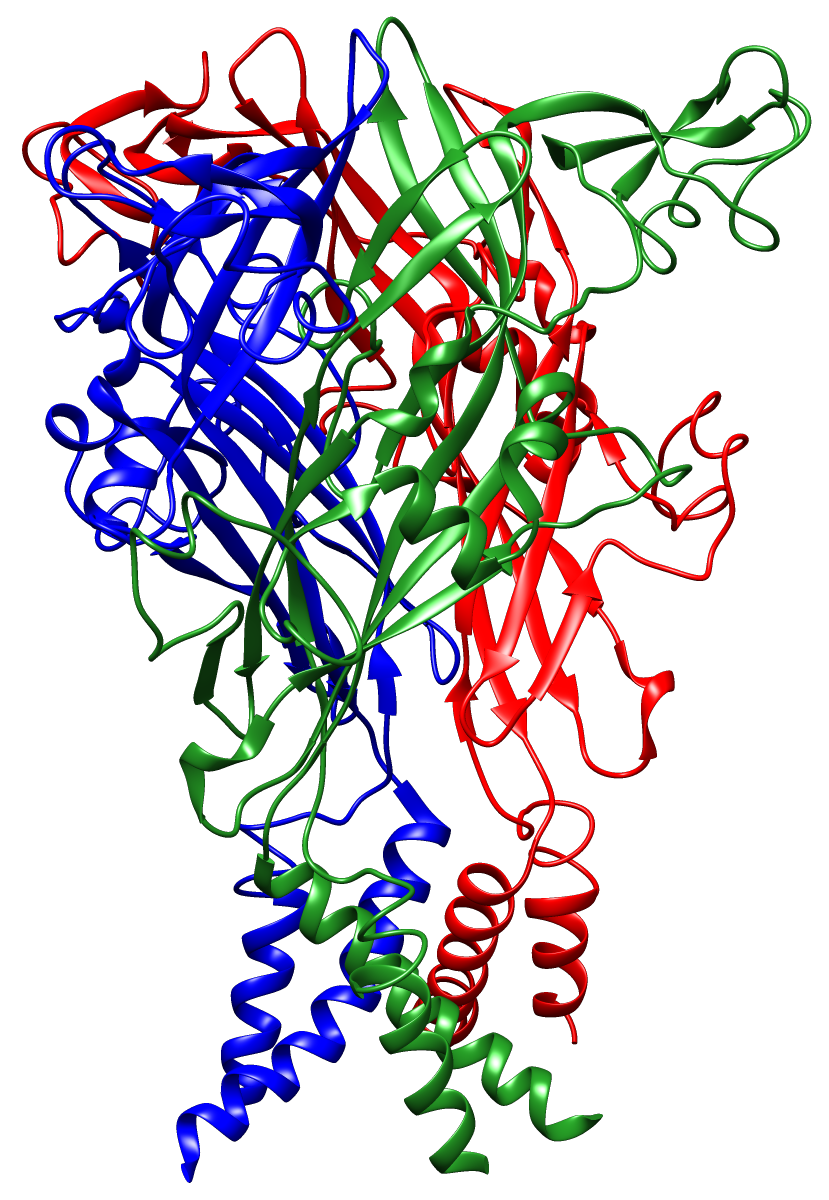
\includegraphics[width=0.5\textwidth]{rysunki/rozdzial_1/p2x.png}%
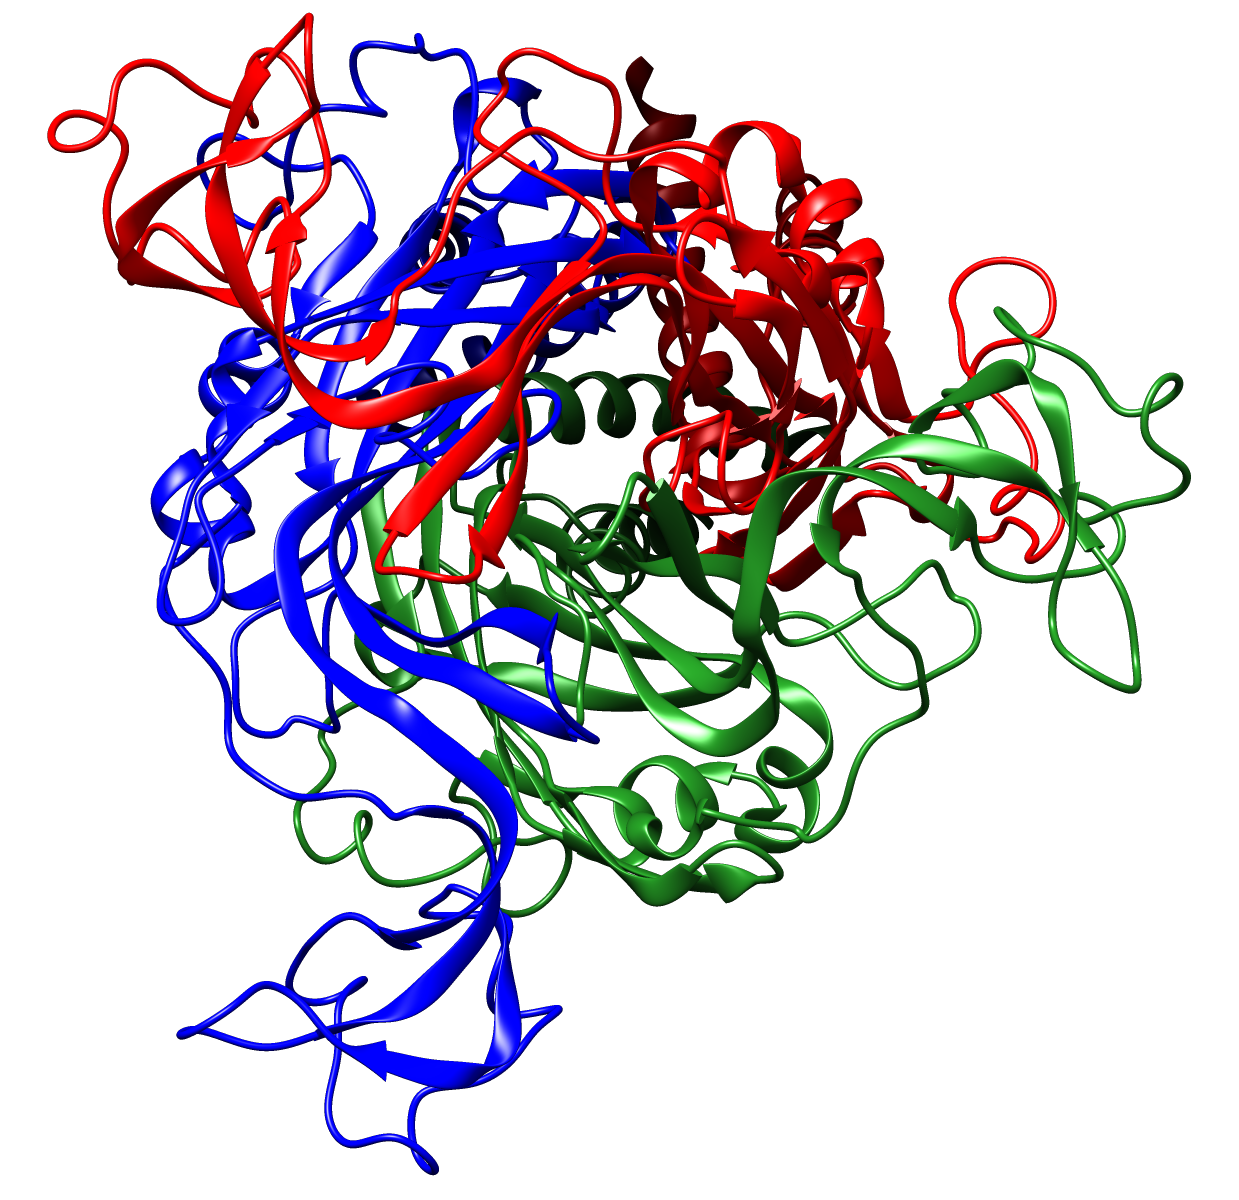
\includegraphics[width=0.5\textwidth]{rysunki/rozdzial_1/p2x2.png}%
\caption [Struktura kanału P2X]{Struktura czwartorzędowa kanału bramkowanego ligandem P2X (kod PDB: \textbf{3I5D}). Kolorami oznaczono poszczególne łańcuchy trimeru \cite{Kawate2009}.}
\label{fig:p2x}
\end{figure}

\begin{figure}[tb]
\centering
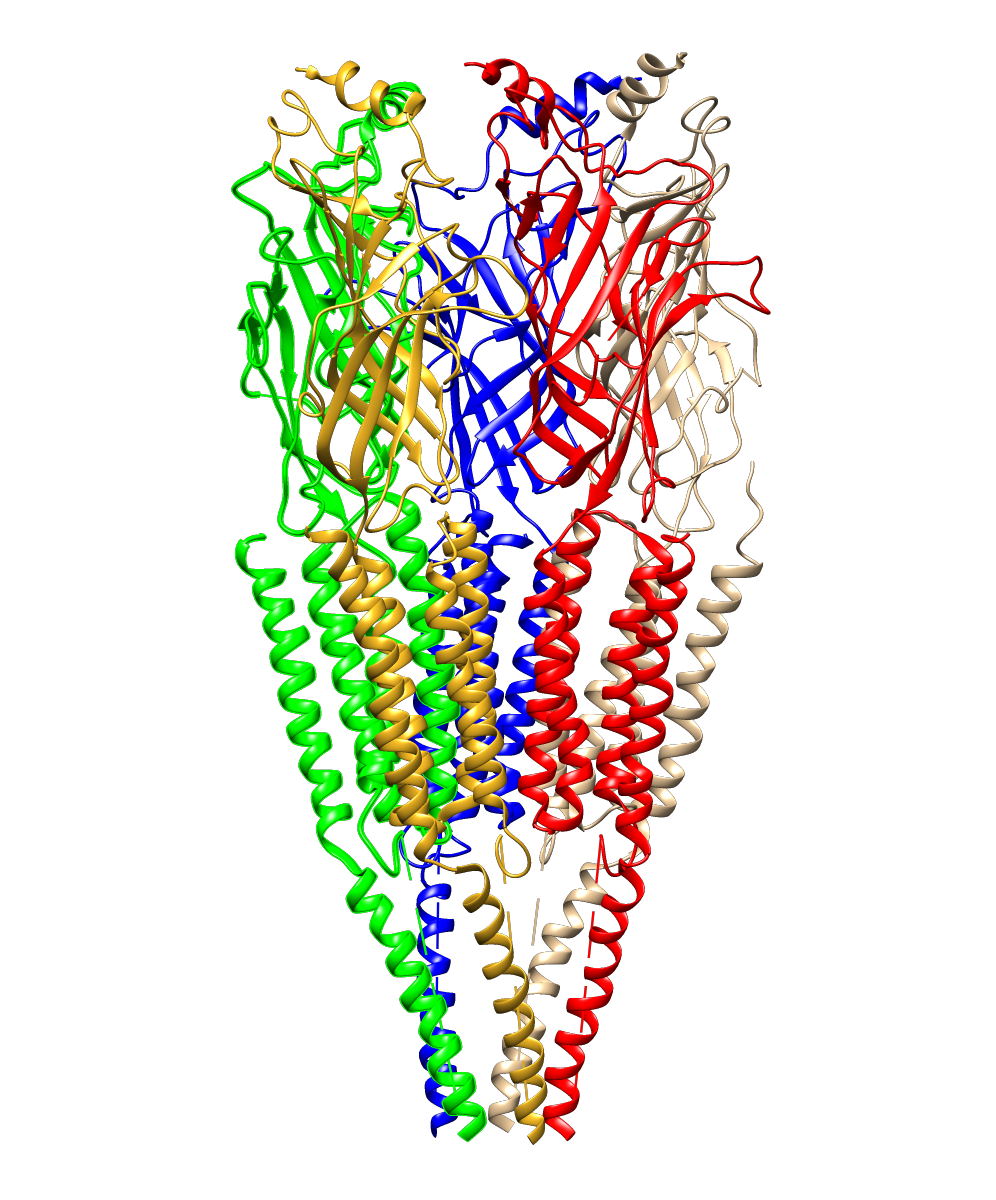
\includegraphics[width=0.45\textwidth]{rysunki/rozdzial_1/2bg9nAChRside.png}%
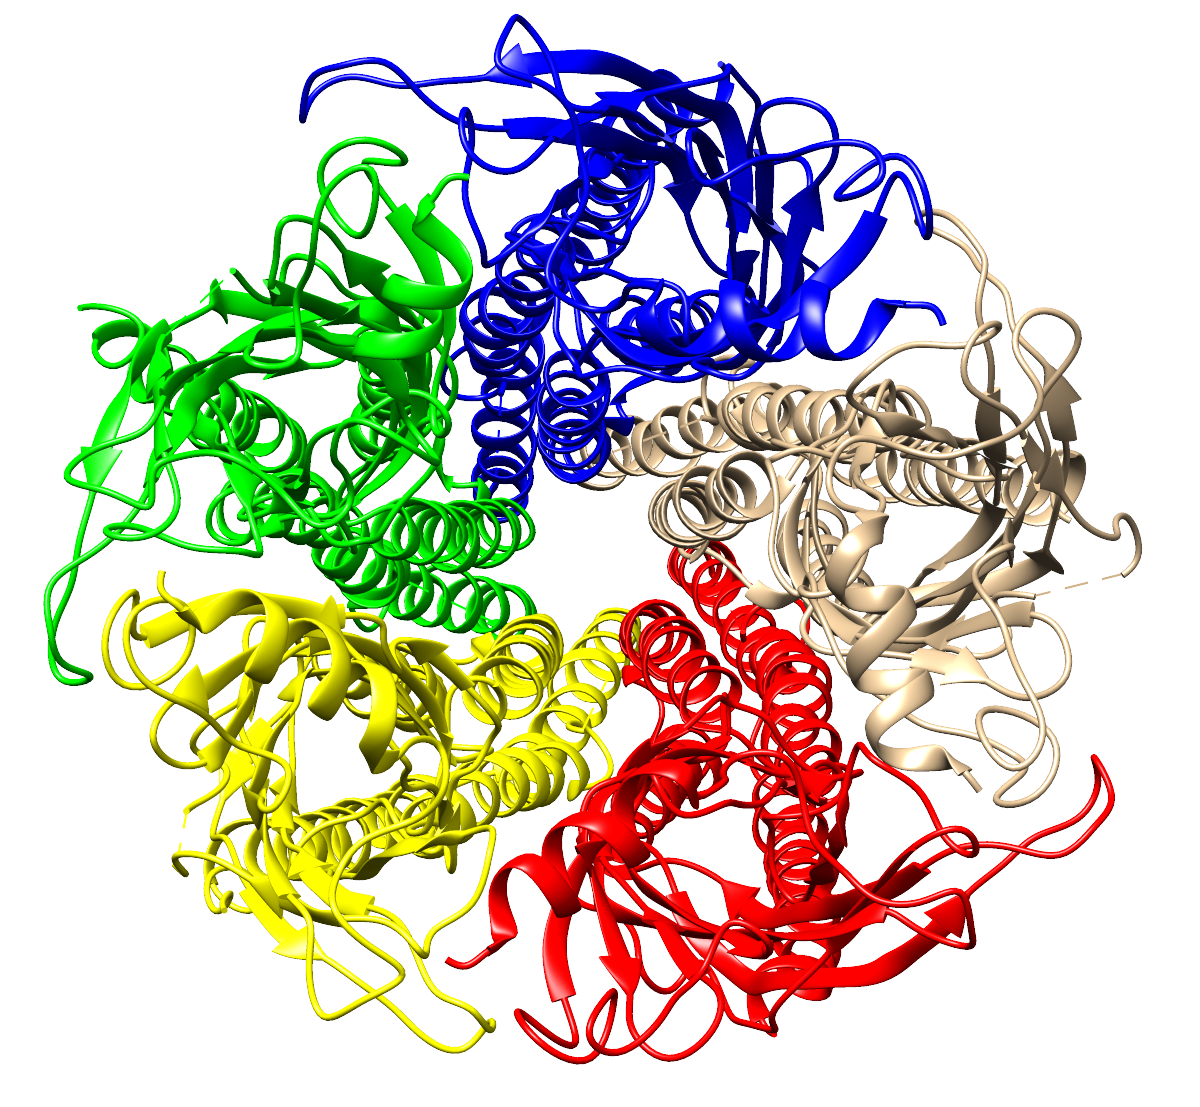
\includegraphics[width=0.45\textwidth]{rysunki/rozdzial_1/2bg9nAChR.png}%
\caption [Struktura kanału nAChR]{Struktura czwartorzędowa kanału nAChR (kod PDB: \textbf{2BG9}). Kolorami oznaczono poszczególne łańcuchy pentameru \cite{Unwin2005}.}
\label{fig:nachr}
\end{figure}

\FloatBarrier
\subsubsection{Pompa plazmatyczna (PMCA)}\label{sss:PMCA}

W komórce obecne są dwa oddzielne mechanizmy usuwania wapnia: za pomocą białka ATPazy, który jest pompę wapniową i wymiennika jonowego. Pozwala to na utrzymanie bardzo niskiego stężenia jonów wapnia w cytozolu, które jest utrzymywane na poziomie 50-100 nM.

\textbf{Pompa wapniowa} zlokalizowana na błonie komórkowej należy do rodziny \mbox{ATPaz} typu P, do której należą trzy rodzaje pomp wapniowych: PMCA (pompy błony komórkowej), SERCA (pompy magazynów wewnątrzkomórkowych) i SPCA (pompy na powierzchni aparatów Golgiego). PMCA składa się z 10 transbłonowych domen, przy czym obydwa końce: NH2, i~COOH znajdują się od strony cytoplazmatycznej. Cytoplazmatyczny fragment pompy zawiera 3 ważne rejony: pętlę cytoplazmatyczną, pełniącą istotną rolę podczas cyklu transportowego, centrum aktywne z asparaginianem w pozycji D465 (ten aminokwas ulega fosforylacji) oraz domeną regulatorową na końcu karboksylowym \cite{DiLeva2008,Guerini2005}.

ATPazy charakteryzuje wysokie powinowactwo do jonów Ca$^{2+}$, mechanizm działania opiera się o wykorzystanie energii zawartej w ATP, która pozwala usunąć wapń z cytoplazmy \cite{Brini2000}. W~trakcie cyklu pracy pompy wytwarzany jest nietrwały związek pośredni, który powstaje z reszty fosforanowej z ATP i reszty asparaginianu, który znajduje się w centrum aktywnym enzymu. W~wyniku fosforylacji enzym zmienia konformację i zmniejsza się jego powinowactwo do jonów wapnia, które pierwotnie wiążą się do domen po cytoplazmatycznej stronie. Zmiana konformacyjna powoduje, że jony wapnia są eksponowane do środowiska zewnętrznego. Zmniejszone powinowactwo powoduje oddysocjowanie jonu. PMCA transportuje jeden jon wapnia podczas jednego cyklu hydrolizy ATP \cite{DiLeva2008}.

Aktywność PMCA regulowana jest na kilka sposobów. Podstawowym mechanizmem jest fosforylacja reszt serynowych, treoninowych i tyrozynowych przez kinazy typu A (PKC) oraz typu A (PKA)\nomenclature{PKA}{kinaza białkowa typu A}. Modyfikacje reszt treoninowych i serynowych zwiększają V$_{max}$ oraz powinowactwo do jonów wapnia, natomiast fosforylacje reszt tyrozynowych hamują aktywność pompy \cite{DiLeva2008}. Aktywność PMCA regulowana jest również przez skład lipidowy otoczenia. W szczególności obecność fosfolipidów: 4,5-difosforan fosfatydyloinozytolu (PIP$_2$)\nomenclature{PIP$_2$}{4,5-difosforan fosfatydyloinozytolu} i fosfatydyloseryny. Obecność tych związków obniża stałą półaktywacji pompy do 100 nM. Pompa wapniowa PMCA wchodzi również w interakcje z szeregiem białek, które modyfikują jej aktywność m. in kalmodulina, kalpainy, oraz rodziny białek posiadających tzw. domenę PDZ \cite{Ranganathan1997}.

\subsubsection{Wymiennik Na$^+$/Ca$^{2+}$ (NCX)}\label{ch:NCX}
\textbf{Wymiennik sodowo-wapniowy} może znajdować się w jednym z dwóch stanów konformacyjnych: w~konformacji skierowanej w stronę przestrzeni miedzybłonowej lub zewnątrzkomórkowej, oraz konformacji skierowanej w~stronę cyzolu/macierzy mitochondrium. Białko posiada trzy miejsca wiązania jonów sodowych i jedno miejsce wiązania jonów wapniowych. Przełączenie pomiędzy konformacjami następuje w~dwóch sytuacjach: kiedy wszystkie miejsca wiązania sodu są związane, a miejsce wiązania wapnia wolne lub kiedy miejsce wiązania wapnia jest zajęte, a miejsca wiązania sodu wolne. Otwarcie nośnika w stronę cytozolu powoduje, że wypełniane są miejsca wiązania jonów wapnia (ze względu na niewielką ilość jonów Na$^+$ w cytozolu). Odwrotnie wygląda sytuacja, kiedy wymiennik znajduje się w konformacji otwartej na zewnątrz komórki. Tam stężenie jonów sodu jest niemal 70 razy wyższe niż stężenie jonów wapnia, więc z~większym prawdopodobieństwem obsadzone zostaną wszystkie miejsca wiązana jonów sodu. W ten sposób wprowadzenie zasad dotyczących możliwości zmiany konformacji wytworzyło nośnik jonów, który wykorzystuje ich potencjał chemiosmotyczny do zamiennego przenoszenia ich w poprzek błony biologicznej \cite{Altimimi2007a}.

\begin{wrapfigure}{o}{0.5\textwidth}
%\vspace{-1cm}\hspace{10pt}
  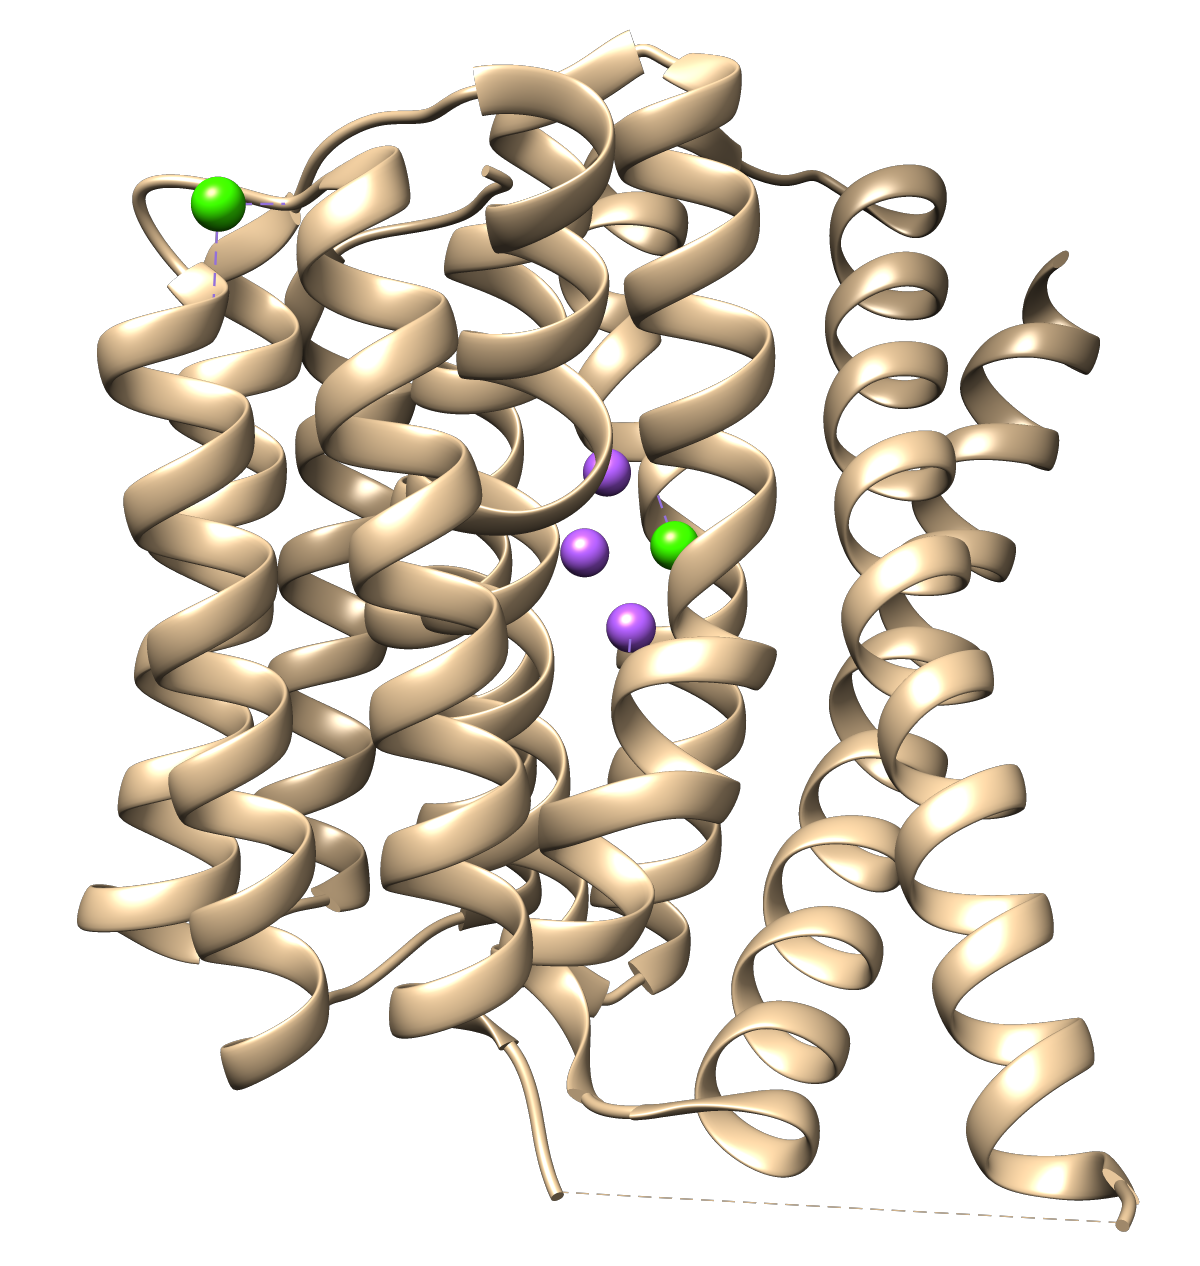
\includegraphics[width=0.5\textwidth]{rysunki/rozdzial_1/ncx.png}
 \caption[Wymiennik NCX]{Schemat wstążkowy przedstawiający strukturę wymiennika sodowo-wapniowego. Zielonym kolorem oznaczone zostały jony Ca$^{2+}$, purpurowym jony Na$^+$ (kod PDB: \textbf{3V5U}) \cite{Liao2012}.}
 \label{fig:NCX}
\end{wrapfigure}

Wymiennik \textbf{NCX} jest zatem typowym przykładem antyportu drugiego rzędu w komórce. Zużywa energię zmagazynowaną w wyniku przeniesienia trzech jonów sodowych do przetransportowania jednego jonu wapnia na zewnątrz komórki.
NCX to wymiennik o bardzo niskim powinowactwie, ale wysokiej sprawności transportowej w stosunku do jonów wapnia. Dlatego ich działanie istotne jest na początku sygnału wapniowego, kiedy stężenie wapnia jest najwyższe. Pozwala to na szybkie usuniecie z cytozolu dużych ilości wapnia. Wykorzystuje ruch do komórkowy ruch jonów sodu zgodny z gradientem stężeń do transportu jonów wapnia wbrew gradientowi \cite{Shibukawa2007}. NCX odgrywa szczególną rolę w komórkach pobudliwych, gdzie z dużą wydajnością usuwa znaczne ilości jonów wapnia, który napływa do cytozolu w trakcie aktywacji na styku synaps lub płytki moto-nerwowej \cite{Annunziato2004}. Oprócz jonów wapnia niektóre przenośniki są w stanie transportować potas. Mówimy wówczas o wymiennikach Na$^+$/K$^+$/Ca$^{2+}$ (\textbf{NCKX}), które stanowią osobną podrodzinę i wymieniają sód na jony potasu i wapnia. U ssaków opisano trzy geny kodujące białka NCX i sześć kodujących białka NCKX \cite{Lytton2007}.


\FloatBarrier
\subsection{Przepływy wapnia w magazynach ER}\label{ss:transportER}

Wypływ wapnia z magazynów wewnątrzkomórkowych aktywowany jest dwoma oddzielnymi mechanizmami. Pierwszy polega na oddziaływania białko-białko i polega na serii zmian konformacyjnych będących efektem tych oddziaływań. Sensory wapnia na powierzchni błony komórkowej (np. kanał Ca$_V$1.1 typu L) oddziałują bezpośrednio z~kanałami uwalniającymi wapń, głównie RyR-1, zmieniając konformacje tego ostatniego. Mechanizm ten występuje główne w~mięśniach szkieletowych i niektórych neuronach podwzgórza \cite{Berridge2012b}. Drugi mechanizm oparty jest o~syntezę przekaźnika drugiego rzędu. Aktywacja receptorów lub kanałów na błonie komórkowej, prowadzi do wytworzenia drugorzędowego przekaźnika dyfundującego w cytozolu i aktywującego uwolnienie wapnia z magazynów wewnątrzkomórkowych. Jednym z głównych przekaźników drugiego rzędu jest sam wapń, który jest w stanie aktywować kanały RyR/IP$_3$R na drodze \textbf{wypływu wapnia indukowanego wapniem} (CICR - ang. \textbf{c}alcium \textbf{i}nduced \textbf{c}alcium \textbf{r}elease). Ten autokatalityczny mechanizm jest podstawą utrzymujących się oscylacji wapniowych. Kolejnym ważnym przekaźnikiem drugiego rzędu jest trójfofsatydylo-1,4,5-inozytolu (IP$_3$) produkowany po wewnętrznej stronie błony komórkowej.

Pobudzenie komórki powoduje aktywacje receptorów błonowych inicjując kaskadę sygnalizacyjną, która uwalnia Ca$^{2+}$ z magazynów wewnątrzkomórkowych. Stężenie jonów wapnia w~cytoplazmie gwałtownie wzrasta. Wzrost ten spowodowany jest uwalnianiem jonów wapnia z~ER za pośrednictwem zlokalizowanych w błonie ER \textbf{receptorów trojfofsatydylo-1,4,5-inozytolu} (IP$_3$R) oraz \textbf{receptorów rianodynowych} (RyR). Uwalnianie jonów wapniowych z ER za pośrednictwem IP$_3$R wymaga związania wtórnego przekaźnika - trojfofsatydylo-1,4,5-inozytolu (IP$_3$), natomiast receptory RyR aktywowane są poprzez wzrost stężenia wapnia w cytozolu (CICR). Impuls aktywujący klaster receptorów może spowodować lokalną zmianę stężenia wapnia w~cytoplazmie, zwaną ,,iskrą Ca$^{2+}$'' (ang. \textit{blip}), ta z kolei powoduje otwarcie kanałów kolejnych klastrów (ang. \textit{,,puf''}) \cite{Foskett2007} i masowy napływ wapnia do cytozolu. Na skutek pobudzenia komórki wzrost jonów wapnia w~cytozolu rośnie do wartości rzędu 0.5--2 $\mu$M.

Osobnym zagadnieniem jest wymiana wapnia między cytozolem i mitochondriami. Wysokie stężenie jonów wapnia w mitochondrium związane jest z obecnością dużego gradientu elektrochemicznego pomiędzy wnętrzem mitochondrium - tzw. macierzy, a~przestrzenią perymitochondrialną, która znajduje się pomiędzy zewnętrzną (OMM)\nomenclature{OMM}{zewnętrzna błona mitochondrium (ang. \textit{\textbf{o}uter \textbf{m}itochondrial \textbf{m}embrane})} wewnętrzną błoną mitochondrium (IMM)\nomenclature{IMM}{wewnętrzna błona mitochondrium (ang. \textit{\textbf{i}nner \textbf{m}itochondrial \textbf{m}embrane})}. Różnica potencjałów nosi również nazwę potencjału błonowego mitochondriów i~określana jest jako $\Delta\Psi_m$. Pobieranie Ca$^{2+}$ przez mitochondria zachodzi przy udziale wyspecjalizowanego kanału wapniowego - uniportera mitochondrialnego, który wykorzystuje potencjał $\Delta\Psi_m$ do przemieszczenia pozytywnie naładowanych jonów do macierzy. Za uwalnianie jonów wapnia z mitochondrium odpowiadają dwa rodzaje transporterów: wymiennik Na$^+$/Ca$^{2+}$ oraz wymiennik H$^+$/Ca$^{2+}$ \cite{Laude2009}.

Jony wapnia uwalniane są z siateczki po aktywacji jednego z rodzajów kanałów wapniowych. W komórkach pobudliwych często występują kanały rianodynowe (RyR), natomiast w~komórkach niepobudliwych receptory IP$_3$ (IP$_3$R).

\subsubsection{Receptor rianodynowy (RyR)}

Receptor rianodynowy (Ryc.~\ref{fig:ryr}) jest bardzo popularnym typem kanału wapniowego, który występuje w większości w komórkach pobudliwych (komórki mięśniowe, kardiomiocyty, komórki Purkinjego). Kanał rianodynowy należy do grupy dużych kanałów jonowych, składa się z czterech monomerów o masie > 2 MDa (każda z czterech podjednostek masę około 550 kDa). RyR zlokalizowany jest w błonie szorstkiej i~gładkiej siateczki śródplazmatycznej \cite{Berridge2012}· Większość tetrameru znajduje się po stronie cytoplazmatycznej (ponad 4/5), a jedynie 1/5 białka stanowią domeny transbłonowe i~fragment luminalny \cite{Wehrens2005}. Receptory rianodynowe sklonowano po raz pierwszy z komórek mięśni szkieletowych \cite{Marks1989,Takeshima1989} i kardiomiocytów \cite{Otsu1990} królika. Wyizolowano trzy izoformy RyR1, RyR2, RyR3 i każda z nich ulega ekspresji na wysokim poziomie w~komórkach mięśni szkieletowych, oraz na niższym poziomie w komórkach nerwowych, jądrach, nadnerczach i jajnikach \cite{Wehrens2005}. Istnieje zróżnicowanie w poziomie ekspresji poszczególnych form, np. RyR1 ulega w większości ekspresji w komórkach mięśni i komórkach Purkinjego móżdżka \cite{Furuichi1994,Hertle2008,Otsu1990,Takeshima1989}, RyR2 ulega ekspresji głównie w~kardiomiocytach [12, 13] i komórkach nerwowych \cite{Hertle2008}, natomiast RyR3 ulega ekspresji głównie w~neuronach kory mózgowej, w obszarze hipokampa i~w~komórkach mięśniowych przepony \cite{Franzini-Armstrong2005,Lanner2012,Mackrill2012}. Sam kanał stanowią domeny transbłonowe, które natywnie tworzą kanał w formie zamkniętej \cite{Kimlicka2013}. Kanały RyR modulowane są przez szereg małych cząsteczek, jonów i białek, do których należą m.in.: Ca$^{2+}$, Mg$^{2+}$, PKA, kalmodulina, FKBP12/12.6, CaMKII, kalsekwestryna. Tworzą one kompleks makromolekularny, który moduluje strukturę tetrameru, za czym idzie przepustowość jonów wapnia.


\begin{figure}[h]
 \begin{center}
	\subfloat[Homotetramer - widok z góry]{%
		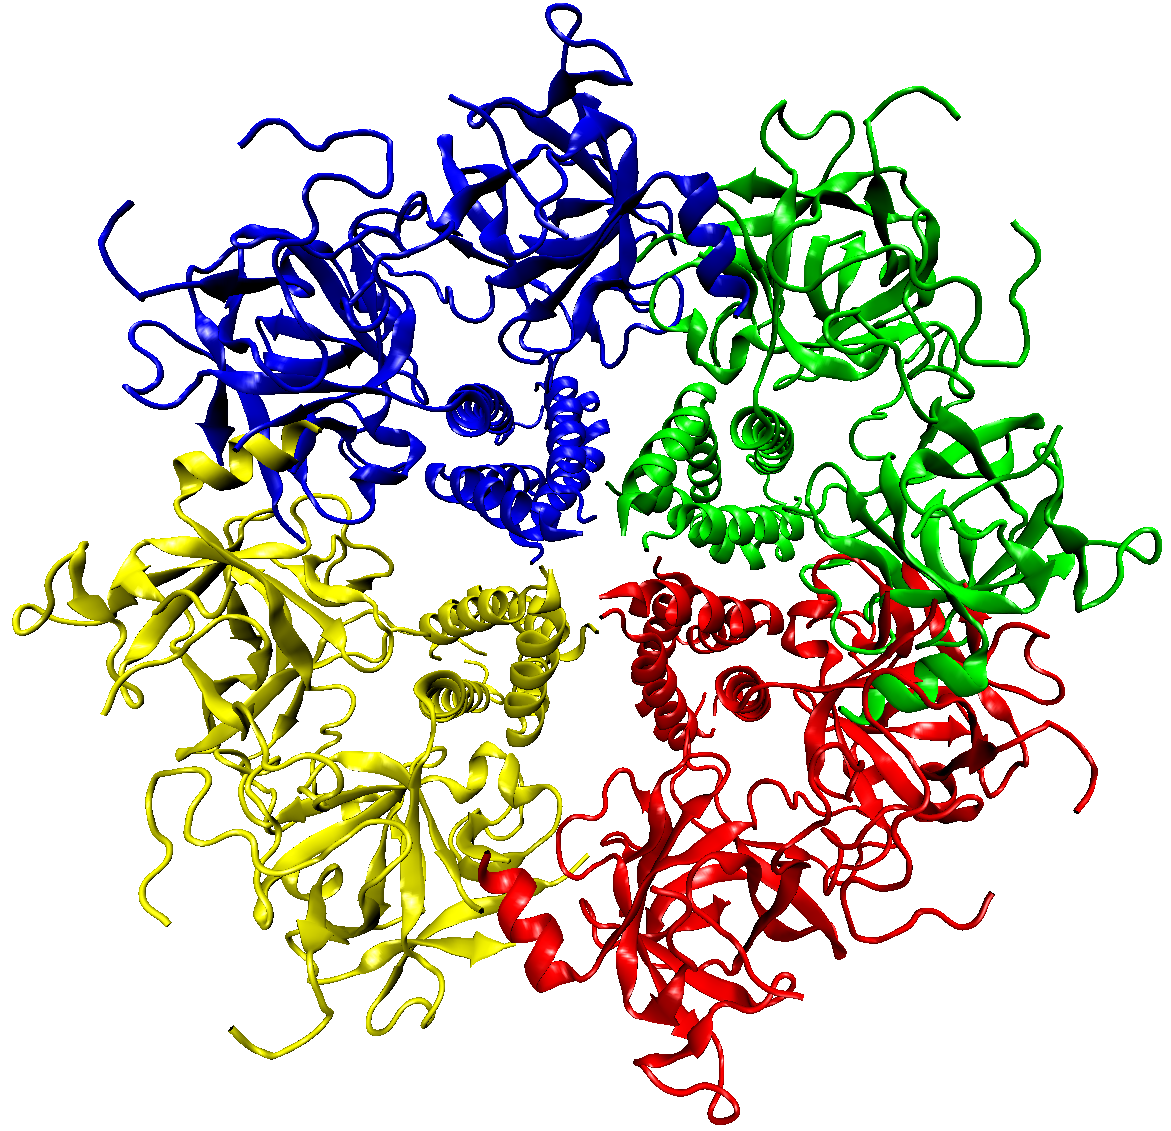
\includegraphics[width=0.5\textwidth]{rysunki/rozdzial_1/ryrtopcolor3.png}%
	\label{fig:RyrLeft}%
	}
	\subfloat[Widok horyzontalny dwóch podjednostek]{%
	\vspace{-3cm}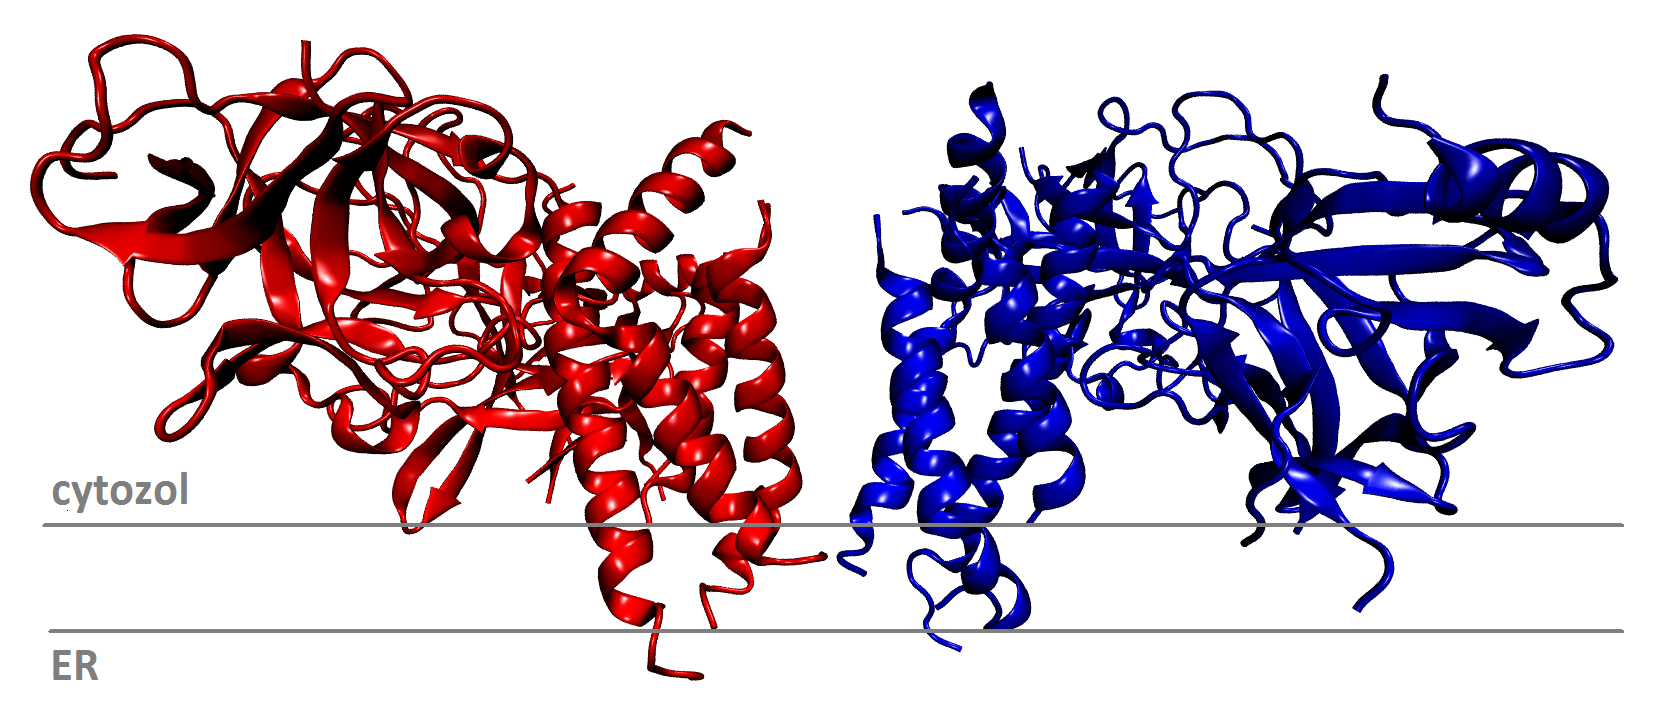
\includegraphics[width=0.5\textwidth]{rysunki/rozdzial_1/ryrhorizontal2.png}%
	\label{fig:RyrRight}%
	}
\end{center}
\caption[Receptor rianodynowy - struktura]{Wstążkowa reprezentacja struktury czwartorzędowej receptora rianodynowego złożonego z czterech podjednostek, które jako homotetramer tworzą kanał wapniowy RyR-1 - dokowanie monomerów przy użyciu oprogramowania \textbf{MultiFit Webserver} \cite{Tjioe2011}. Kod PDB monomeru: \textbf{2XOA} \cite{Tung2010}, kod EMDB mapy gęstości elektronowej \textbf{EMDB-1606} \cite{Samso2009}.}
\label{fig:ryr}
\end{figure}

\begin{figure}[tb]
 \begin{center}
  \subfloat[Widok z góry.]{%
  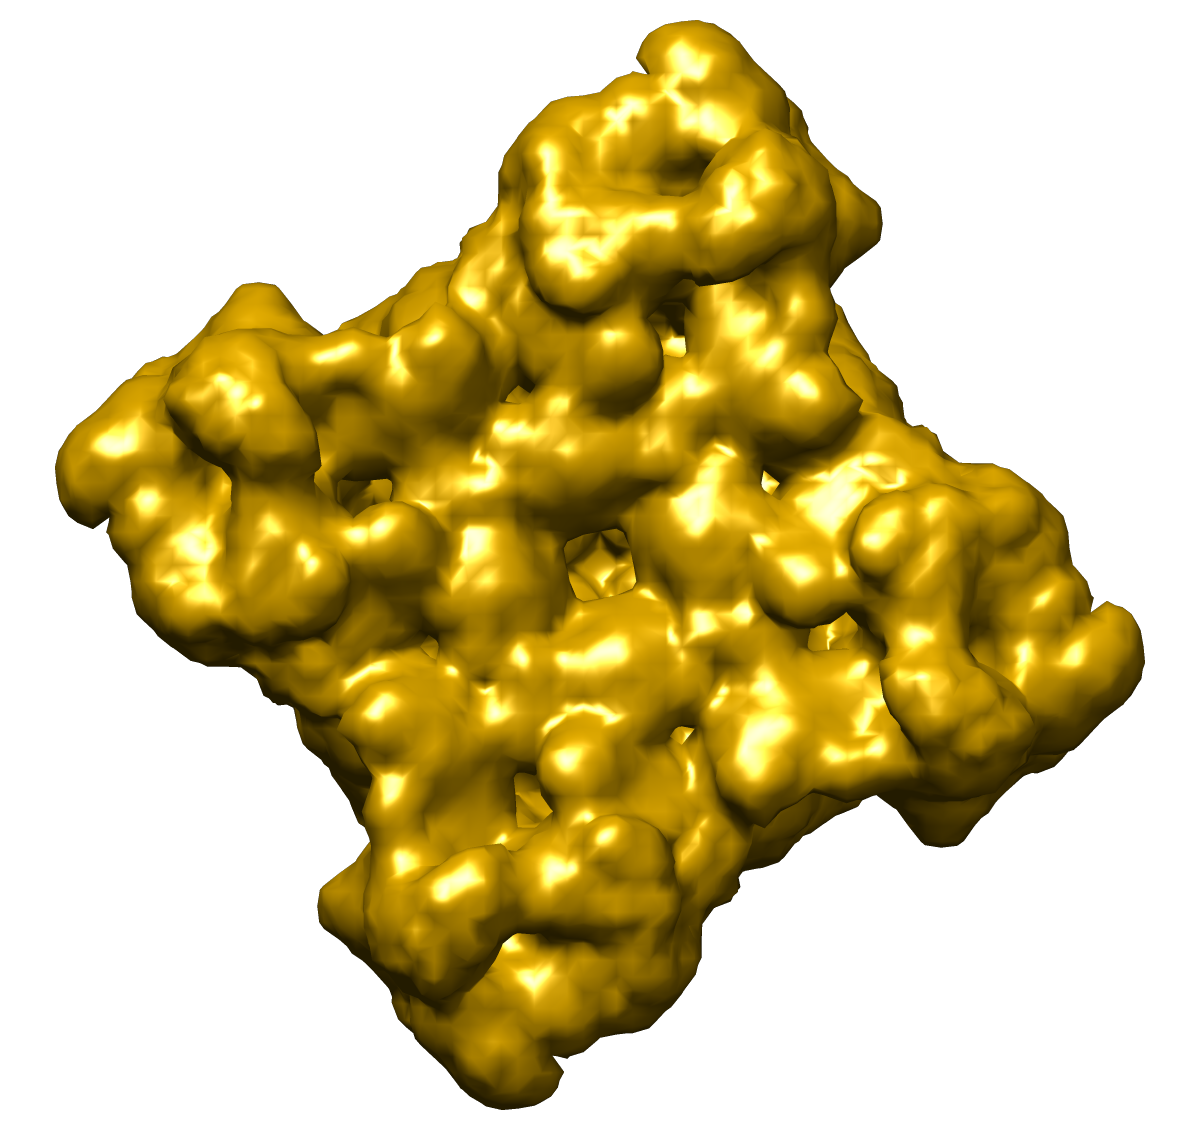
\includegraphics[width=0.47\textwidth]{rysunki/rozdzial_1/ryrcryoem.png}
  }
  \subfloat[Widok z boku]{%
  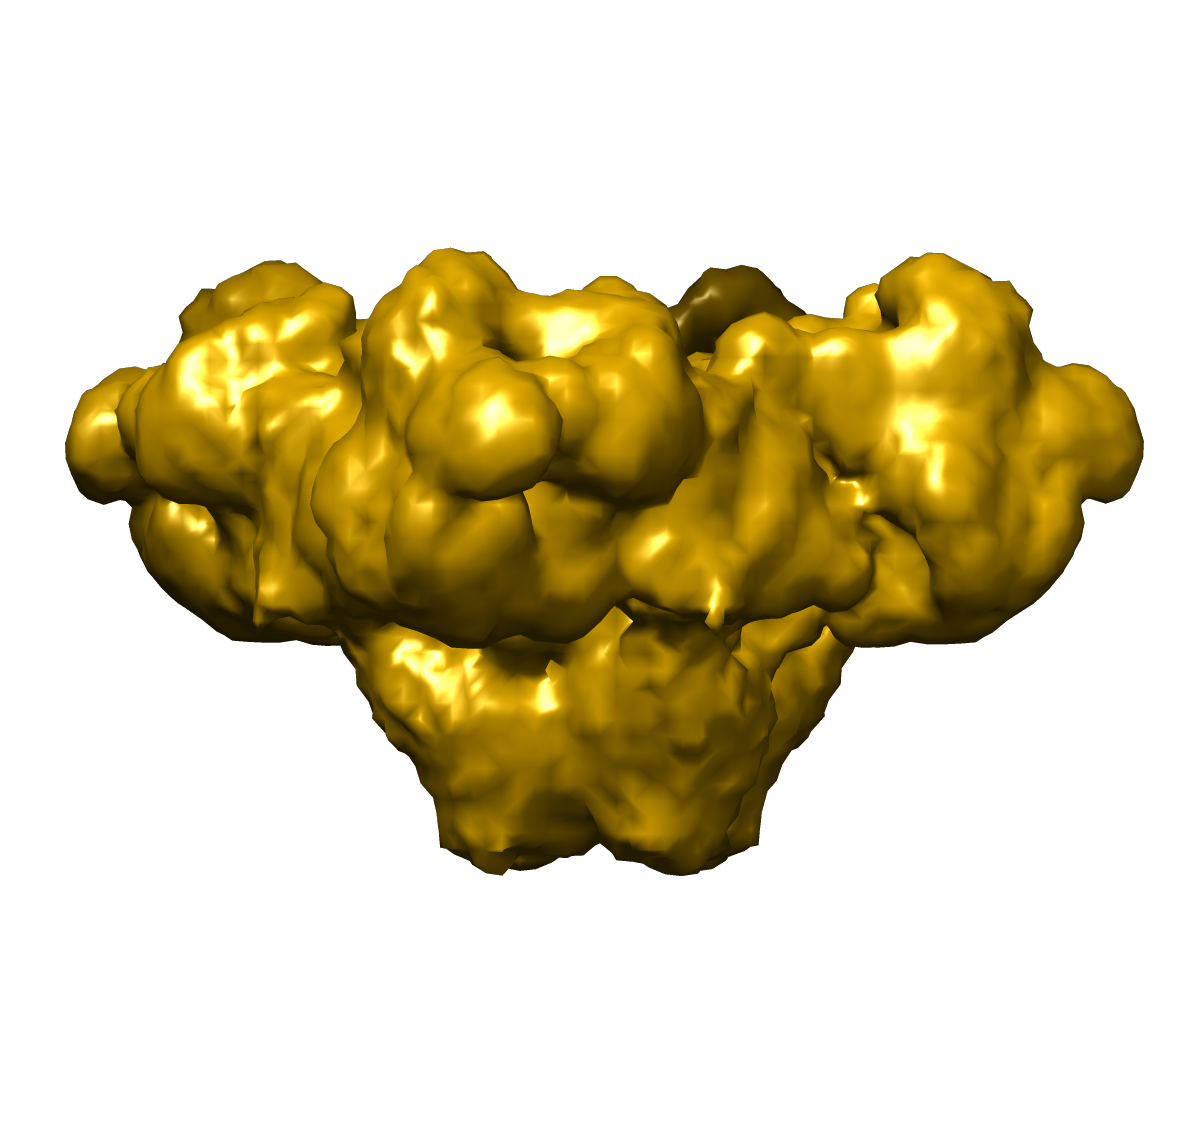
\includegraphics[width=0.47\textwidth]{rysunki/rozdzial_1/ryrcryoem2.png}
  }
 \end{center}
 \caption[Mapa gęstości elektronowej receptora RyR1]{Mapa gęstości elektronowej receptora rianodynowego RyR-1 w stanie zamkniętym, uzyskana metodą cryo-EM (kod EMDB: \textbf{EMDB-1606}) \cite{Samso2009}. Mapa gęstości elektronowej pozwala określić kształt cząsteczki.}
 \label{fig:RyRcryo}
\end{figure}

Domena N-terminalna zawiera miejsca wiązania szeregu modulatorów (np. białka FKBP12/12.6), które wiążą się do kanału wapniowego w konformacji zamkniętej i stabilizuje go.


\FloatBarrier
\subsubsection{Receptor IP$_3$ (IP$_3$R)}

Aktywacja komórek przez czynniki pozakomórkowe (agonistów) może prowadzić do aktywacji białek G, co z kolei  prowadzi do wytworzenia 1,4,5-trifosforanu inozytolu (IP$_3$). IP$_3$ jest uważany za ogólny przekaźnik drugiego rzędu, który łatwo dyfunduje w cytozolu. Jego receptor - IP$_3$R jest z kolei kanałem uwalniającym jony wapnia do cytozolu (Rozdz. ~\ref{ss:transportER}). Kanał ten usytuowany jest na błonie retikulum endoplazmatycznego szorstkiego i gładkiego (ER). Jednym z najważniejszych czynników kontrolujących aktywność IP$_3$R są jony wapnia obecne po cytozolicznej stronie kanału. Dlatego też określane są czasem jako ko-agonista tego kanału. W stężeniach do 300 nM obecność jonów wapnia po cytozolicznej stronie znacznie zwiększa przepuszczalność kanału dla tych jonów. W wyższych stężeniach wapń hamuje aktywność białka \cite{Parys2012}. W~organizmach wyższych odkryto trzy podstawowe izoformy kanału kodowane przez trzy różne geny. Różne izoformy posiadają bardzo podobną strukturę i funkcję. Różni je wrażliwość na poszczególne regulatory, czy lokalizacja subkomórkowa. Białko odkryto w latach 80-tych poprzedniego stulecia. Pierwsze doświadczenia z białkiem początkowo określanym jako P4000 od razu skojarzone zostało z mechanizmem zwiększania ilości wapnia w cytozolu. 

\begin{figure}[h]
	 \begin{center}
	 	\subfloat[Widok z góry.]{ %
	 		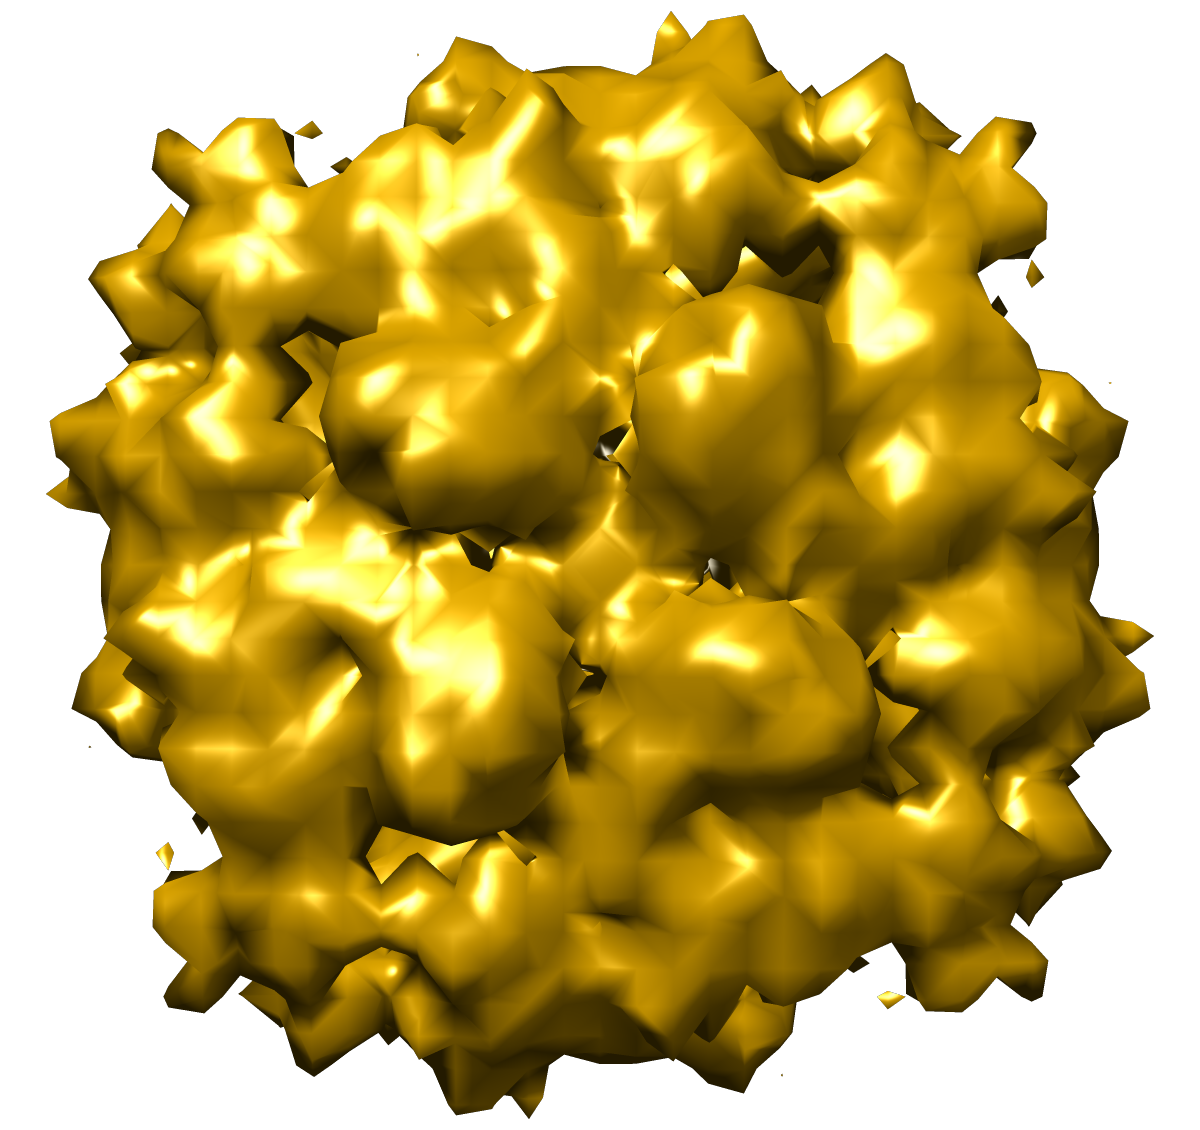
\includegraphics[width=0.47\textwidth]{rysunki/rozdzial_1/ip3cryoem.png}
	 	}
	 	\subfloat[Widok z boku]{%
	 		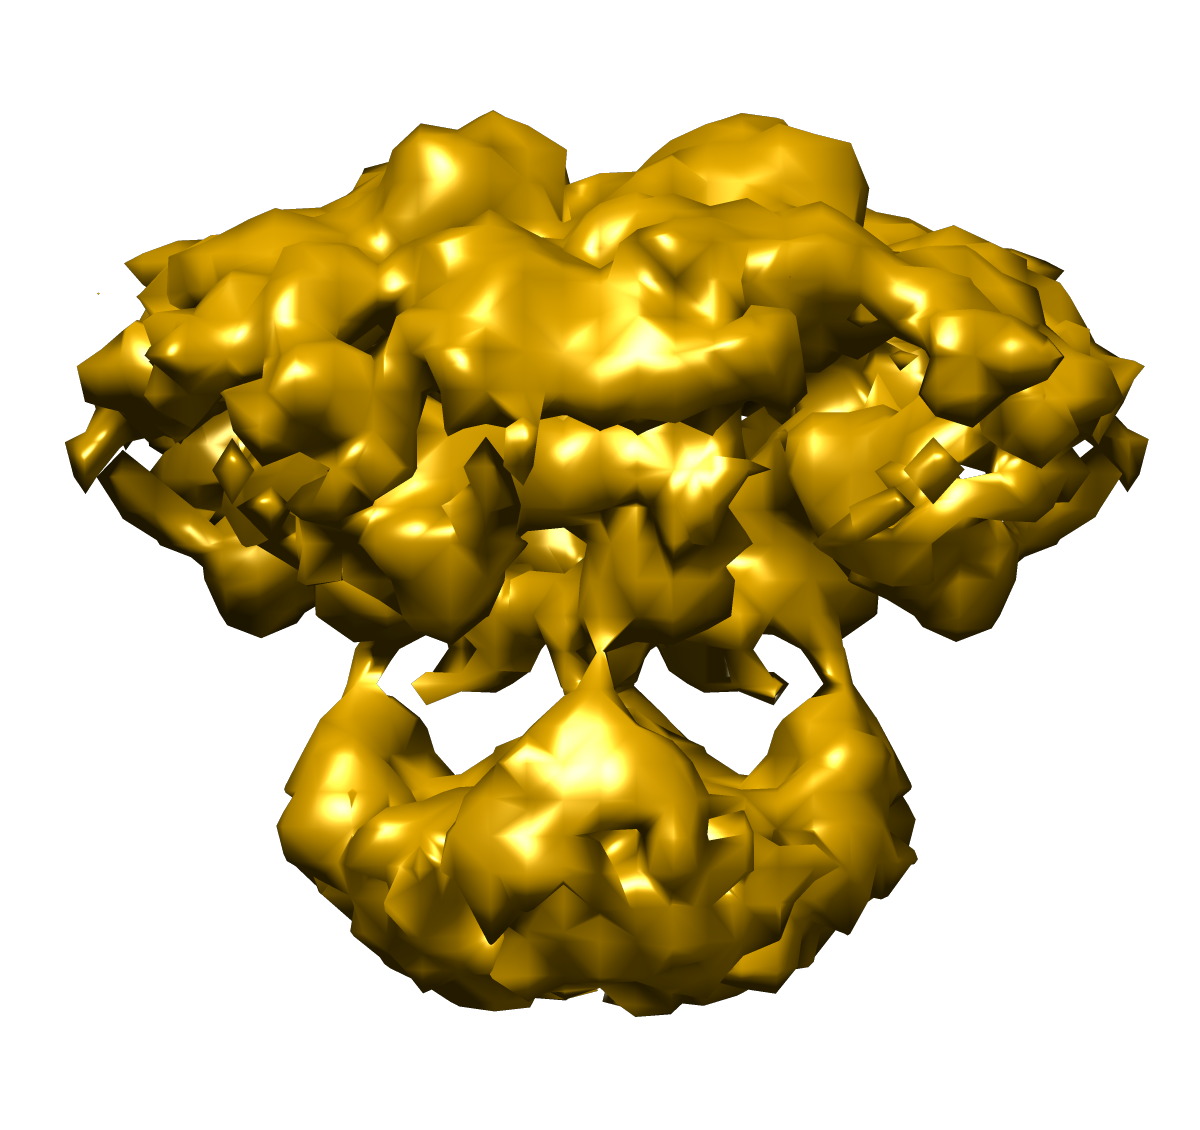
\includegraphics[width=0.47\textwidth]{rysunki/rozdzial_1/ip3cryoem2.png}
	 	}
	 \end{center}
	\centering
	\caption[Mapa gęstości elektronowej receptora IP$_3$R]{Mapa gęstości elektronowej receptora inozytolo-3,4,5-trifosforanu (kod EMDB: \textbf{EMD-5278}) \cite{Seo2012}.}
	\label{fig:IP3Rcryo}
\end{figure}


Wykazano, że w przypadku organizmów zmutowanych, u których ekspresja P4000 nie występuje lub jest znacznie zredukowana dochodzi do szeregu zaburzeń OUN - obumieranie komórek Purkinjego, znacznie zredukowany rozrost dendrytów. Immunoprecypitacja pozwoliła wyizolować białko i dopiero w latach 90-tych udało się wyizolować samo białko i przeprowadzić analizę genetyczną. Sklonowano cDNA o długości 2700 aa, czyli $\sim$10 kpz. Oczyszczone białko zostało zanalizowane i~po wkomponowaniu w~dwuwarstwę lipidową okazało się działać jako kanał wapniowy \cite{Mikoshiba2012}. Strukturę krystaliczną jądra kompleksu IP$_3$R z ligandami określono w 2002 roku \cite{Bosanac2002}. Analiza struktury wykazała, że każda z izoform charakteryzuje się innym powinowactwem białka w stosunku do IP$_3$. Domena odpowiedzialna za wiązanie IP$_3$ znajduje się w pobliżu N-końca. Jądro kompleksu obejmuje aminokwasy od 226-558 i jest to podstawowa funkcjonalna jednostka odpowiedzialna za wiązanie trifosforanu inozytolu. 
Badania mutantów receptora IP$_3$R wskazują na jeden wspólny typ dysfunkcji, który pojawia się po upośledzeniu funkcji kanału lub jego wyciszeniu, czyli występowanie zaburzeń funkcji OUN, napady padaczkowe, obniżona plastyczność neuronalna. Myszy, u których sztucznie wywołano podwójny nokaut genu IP$_3$R (IP$_3$R$^{-/-}$) ginęły krótko po narodzinach \cite{Katsuhiko2007}.

\FloatBarrier
\subsubsection{Pompa sarko-endoplazmatyczna (SERCA)}

Pompa wapniowa jest ATP-azą typu P, która transportuje jony wapnia w kierunku wyższego gradientu gradientu stężenia jonów wapnia w świetle ER. Energia do transportu pochodzi z hydrolizy ATP. Na każdą cząsteczkę ATP zużytą do zmiany konformacji przypadają dwa jony wapnia przetransportowane z cytozolu do ER.


%Tutaj mamy rozwiązał struktury krystalicznej ATPazy wapniowej mięśni szkieletowych sarkoplazmatycznej (SERCA1a) 2,6 AE
%Rezolucja z dwóch jonów wapnia związany w domenie, która zawiera transmembranowej alfa-helisy. Dwa jony wapnia są
%położone obok siebie i są otoczone przez czterech helis transbłonowych, z których dwa są rozwijana przez ef koordynacji ® tywnego
%geometria.Region składa się z trzech cytoplazmy dobrze rozdzielonych domen, z miejscem fosforylacji w centrum katalitycznego
%domeny i miejsce wiązania adenozyny na innej domenie.Domeny fosforylacji ma taką samą krotność haloacid
%dehalogenase. Porównanie z niskiej rozdzielczości mapy gęstości elektronów enzymu przy braku wapnia oraz
%Dane biochemiczne wskazują, że duże ruchy domen odbywa się podczas aktywnego transportu.
%
%Za wytworzenie tak dużego gradientu stężenia jonów pomiędzy cytozolem a ER odpowiada ATP-aza SERCA zlokalizowana w błonie ER, aktywnie pompująca jony wapnia do światła siateczki śródplazmatycznej.
%Wapń transportowany jest do wnętrza retikulum przez retikularną pompę wapniową - SERCA. Na każdą cząsteczkę ATP zużyta do zmiany konformacji przypadają dwa jony wapnia przetransportowane z cytozolu do ER.


\begin{figure}[h]
 \begin{center}
  \includegraphics[width=0.45\textwidth]{rysunki/rozdzial_1/serca.png}
  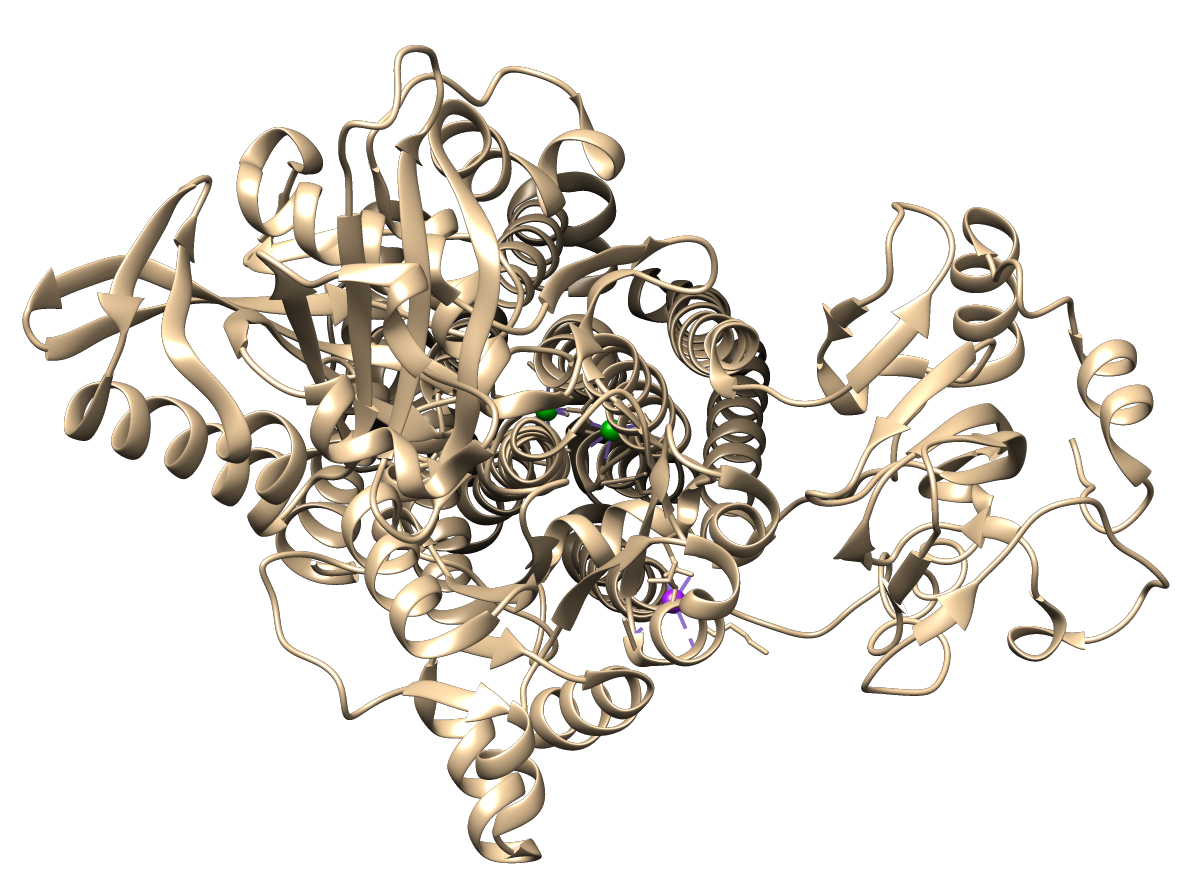
\includegraphics[width=0.52\textwidth]{rysunki/rozdzial_1/serca2.png}
 \end{center}
 \caption[Pompa wapniowa SERCA]{Schemat wstążkowy struktury trzeciorzędowej pompy wapniowej SERCA komórek mięśniowych (kod PDB: \textbf{1SU4})\cite{Toyoshima2000}.}
 \label{fig:SERCA}
\end{figure}


Mechanizm działania SERCA oparty jest o czterostopniowy model. Miejsce hydrolizy ATP położone jest blisko asparaginianu 351, który odbiera resztę fosforanową z~ATP. Miejsce hydrolizy jest znacznie oddalone od miejsca transportowego, wiec kontrola stanu pompy zachodzi w wyniku dużych ruchów domeny wiążącej ATP, która otwiera i zamyka kanał, przez który przechodzi wapń. SERCA transportuje również H$^+$. Jeden cykl przenosi dwa jony wapnia do lumen i cztery jony wodoru do cytoplazmy \cite{Laude2009}.

Pompa SERCA występuje głównie w błonie siateczki śródplazmatycznej oraz sarkoplazmatycznej. Podobnie jak wszystkie ATPazy typu P posiada 10 transbłonowych domen z końcami -NH$_2$ oraz -COOH ułożonymi po stronie cytoplazmatycznej. Aktywacja następuje w wyniku fosforylacji reszty asparaginowej znajdującej się w centrum aktywnym enzymu. SERCA nie zawiera obszaru dodatnio naładowanych reszt w obrąbie pierwszej pętli cytoplazmatycznej, co sprawia, że w przeciwieństwie do PMCA nie oddziałuje z kwasowymi fosfolipidami. Miejsce aktywne znajdujące się w drugiej pętli cytoplazmatycznej zawiera kwas asparaginowy ulegający fosforylacji (patrz Rozdz. \ref{sss:PMCA}) \cite{Brini2000,Lopreiato2014}.


\subsection{Przepływy wapnia w magazynach mitochondrialnych}\label{ss:transportmito}


\begin{figure}[tb]
 \begin{center}
  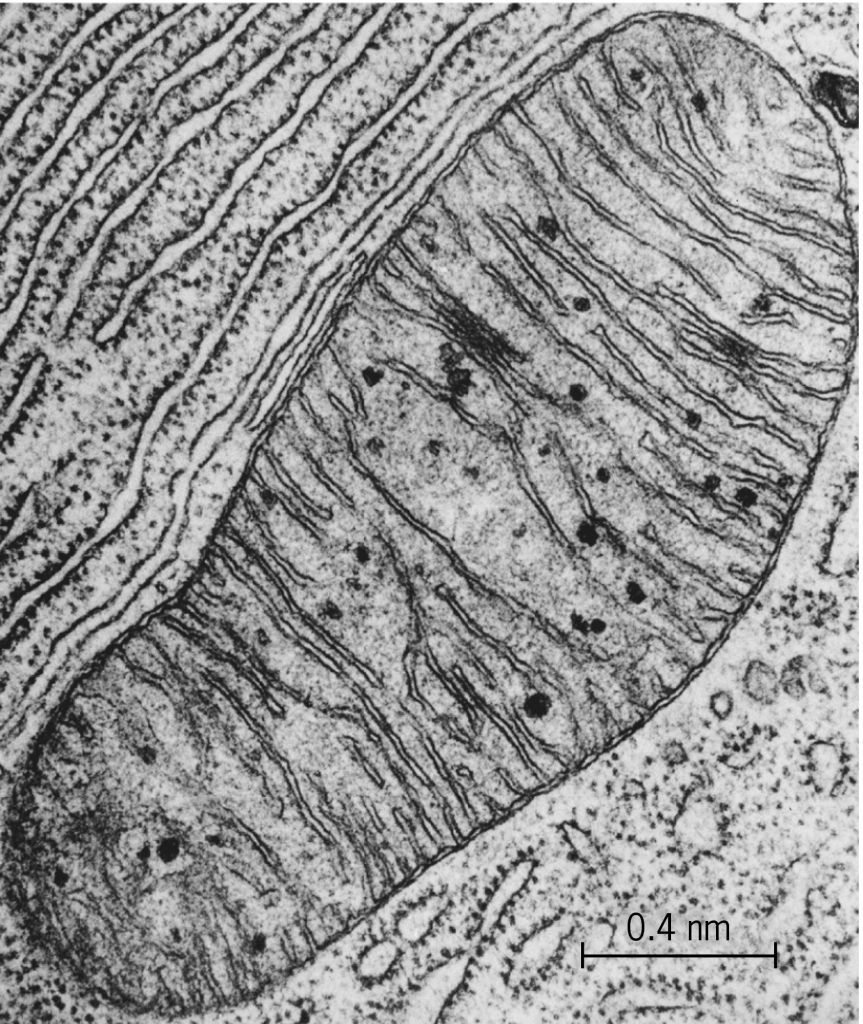
\includegraphics[width=0.95\textwidth]{rysunki/rozdzial_1/mitochondrium.jpg}
 \end{center}
 \caption[Mitochondrium i ER - mikrografia]{Mitochondrium i siateczka śródplazmatyczna szorstka - mikrografia~\cite{Scheffler1999}.}
 \label{fig:mitoER}
\end{figure}

Mitochondria mogą przyjmować w komórce różnorodne kształty. Od małych globularnych struktur do skomplikowanych sieci tubul. Na początku lat osiemdziesiątych, kiedy identyfikowane były podstawowe elementy odpowiedzialne za homeostazę wapniową rola mitochondriów została ograniczona. Uważano, że stanowią magazyn o~dużej pojemności, który aktywuje się w~sytuacjach patologicznych, gdy jony wapnia ,,przeładują'' cytozol. Uwaga badaczy skierowała się na badaniu aktywności siateczki śródplazmatycznej. Sytuacja zmieniła się, kiedy zaczęto oznaczać poziom wapnia bezpośrednio w macierzy mitochondrialnym. Użycie białka hybrydowego - sensora wapniowego aequoryny i mitochondrialnej sekwencji kierunkowej pozwoliło na precyzyjne pomiary wskazujące, że wzrost poziomu wapnia w mitochondrium odbywa się równolegle ze wzrostem wapnia w cytozolu zanim poziom wapnia osiągnie wielkość progową dla uniportera \cite{Rizzuto2000}. Równolegle podobne wyniki uzyskano wykorzystując znaczniki fluorescencyjne z pozytywnym ładunkiem, które lokowały się w macierzy mitochondrialnym ze względu na negatywny ładunek po wewnętrznej stronie IMM (np. rhod-2) \cite{Jou1996}. Od ponad dekady wykorzystywane są również białka wrażliwe na obecność jonów wapnia na bazie GFP \cite{Nagai2001}, które pozwalają na śledzenie niewielkich zmian stężenia wapnia. Zastosowanie tych metod pozwoliło na dokładne zbadanie rzeczywistych zmian stężenia wapnia w komórce i zbadanie dynamiki wymiany wapnia dla poszczególnych kompartmentów. Stosując te metody wykazano, że napływ wapnia aktywowany np. agonistą wiąże się również z następującym po nim wzroście stężenia jonów Ca$^{2+}$ w~mitochondrium. Proces ten ma miejsce zarówno w komórkach pobudliwych (np. kardiomiocyty \cite{Trollinger1997}), jak i~komórkach niepobudliwych (hepatocyty, HeLa \cite{Rizzuto1994,Thomas1991}).


\subsubsection{Mitochondrialny uniporter}
\label{ss:uniporter}

\begin{figure}[tb]
\centering
\includegraphics[width=0.95\textwidth]{rysunki/rozdzial_1/micu1.png}
\caption[Mitochondrium i ER - mikrografia]{Struktura trzeciorzędowa heksameru MICU1, kontrolującego pobór jonów wapnia przez uniporter mitochondrialny (kod PDB: \textbf{4NSC})~\cite{Wang2014}.}
\label{fig:micu1}
\end{figure}


Mitochondrialny uniporter wapniowy (MCU \textit{ang. \textbf{m}itochondrial \textbf{c}alcium \textbf{u}niporter})\nomenclature{MCU}{mitochondrialny uniporter wapniowy (ang. \textit{\textbf{m}itochondrial \textbf{c}alcium \textbf{u}niporter})} odpowiedzialny jest za pobieranie jonów wapniowych z cytozolu komórki do macierzy mitochondrium. Główną siłę napędową funkcjonowania uniportera jest gradient elektrochemiczny w poprzek wewnętrznej błony mitochondrialnej, zwany $\Delta\Psi_m$ = -180mV. Ponieważ wewnętrzna strona IMM naładowana jest ujemnie, transport pozytywnie naładowanych jonów Ca$^{2+}$ kierowany jest do wnętrza mitochondrium. Każdemu przeniesionemu przez IMM jonowi wapniowemu towarzyszy spadek potencjału elektrycznego $\Delta\Psi_m$. Badania techniką ,,patch-clamp'' wykazały, że białko uniportera jest w stanie tworzyć kanał wapniowy, selektywny dla jonów wapniowych \cite{Kirichok2004}. Obecność selektywnego kanału wapniowego na wewnętrznej błonie mitochondrialnej postulowana już wcześniej, kiedy w latach 80-tych po raz pierwszy zaobserwowano kanał o przewodnictwie elektrycznym ok. 20 pS. Izolacja glikoproteiny o masie 40 kDa pozwalała na rekonstytucję takiego kanału do sztucznych błon lipidowych \cite{Debska-Vielhaber2006}.

Dane eksperymentalne ostatnich lat potwierdzają, że uniporter mitochondrialny składa się z~wielu podjednostek, które pełnią różne funkcje, organizując transport jonów wapnia przez wewnętrzną błonę mitochondrialną. Trzon kanału stanowi podjednostka \textbf{MCU}, która może występować w alternatywnej formie - \textbf{MCUb}~\cite{Raffaello2012}. Z~niektórych prac wynika, że MCU oraz MCUb tworzą por przewodzący jony wapnia \cite{Chaudhuri2013}. \textbf{MICU1} to podjednostka o masie 50kDa, regulująca przepustowość kanału, która posiada w swojej strukturze dwa kanoniczne motywy EF-hand \cite{Perocchi2010}, które przyłączają jony wapnia (po jednym dla każdego motywu) i szereg niekanonicznych, które prawdopodobnie nie posiadają tej funkcjonalności \cite{Wang2014}. Podjednostka ta zlokalizowana została po stronie matrix mitochondrium \cite{Hoffman2013}. Pojawiły się również doniesienia o istnieniu podjednostek regulatorowych \textbf{MCUR1} i \textbf{EMRE}, które mogą kontrolować przepustowość kanału \cite{Chaudhuri2013,Sancak2013}. Mechanizm otwierania i zamykania kanału został niedawno opisany przez Wanga i współpracowników \cite{Wang2014}. MCU i MCUb tworzą por, który połączony jest z heksamerem powstałym po połączeniu podjednostek MICU1. Zgodnie z modelem przedstawionym przez Wanga w takiej formie kanał pozostaje zamknięty. \cite{Wang2014}. Białko MICU1 może przyłączyć dwa jony wapnia, które zmieniają jego konformację i~odsłaniają miejsca interakcji z drugą, analogiczna podjednostką (MICU1+Ca$^{2+}$). Podjednostki w dimerze oddziałują ze sobą silniej, niż podjednostki w heksamerze, więc w~obecności jonów wapnia i formowanie się dimerów jest raczej nieuniknione. Dimery mogą tworzyć oligomery za sprawą C-końca MICU1, który pozwala im łączyć się ze sobą. Otwarcie kanału następuje po destabilizacji heksameru MICU1+Ca$^{2+}$ \cite{Wang2014}.

Dalsze mechanizmy oddziaływania dimerów lub oligomerów MICU1 + Ca$^{2+}$ z podjednostką są obecnie przedmiotem badań i stopniowo ujawniane są kolejne szczegóły mechanizmu kontroli aktywności tego kanału wapniowego. Wiadomo jest, że MICU1 kontroluje poziom aktywacji kanału uniportera i jego przepustowość, która jest zależna od obecności jonów wapnia w~środowisku \cite{Csordas2013}. Jednak mechanizm regulacyjny przepustowości uniportera mitochondrialnego wydaje się być o wiele bardziej złożony w~świetle doniesień Patrona i współpracowników \cite{Patron2014}, którzy opisują oddziaływanie paralogu MICU1, stanowiącego kolejną podjednostkę regulatorową - \textbf{MICU2} (Ryc.~\ref{fig:micu2control}). MICU2 różni się od swojego poprzednika masą molekularna (45 kDa) i dzieli z nim około 42 \% sekwencji białkowej \cite{Patron2014}. Wg. autorów zarówno MICU1 i~MICU2 regulują pobieranie wapnia przez uniporter. MICU1 ma niewątpliwie efekt stymulujący na aktywność transportera. MICU2 zaś ma wpływ hamujący aktywność kanału. Razem tworzą heterodimer o masie 95 kDa \cite{Csordas2013,Mallilankaraman2012}. Dodatkowo Plovanich i współpracownicy, używając metod bioinformatycznych, zidentyfikowali kolejny paralog MICU1, który nazwali \textbf{MICU3} \cite{Plovanich2013}.

\begin{figure}[ht]
\centering
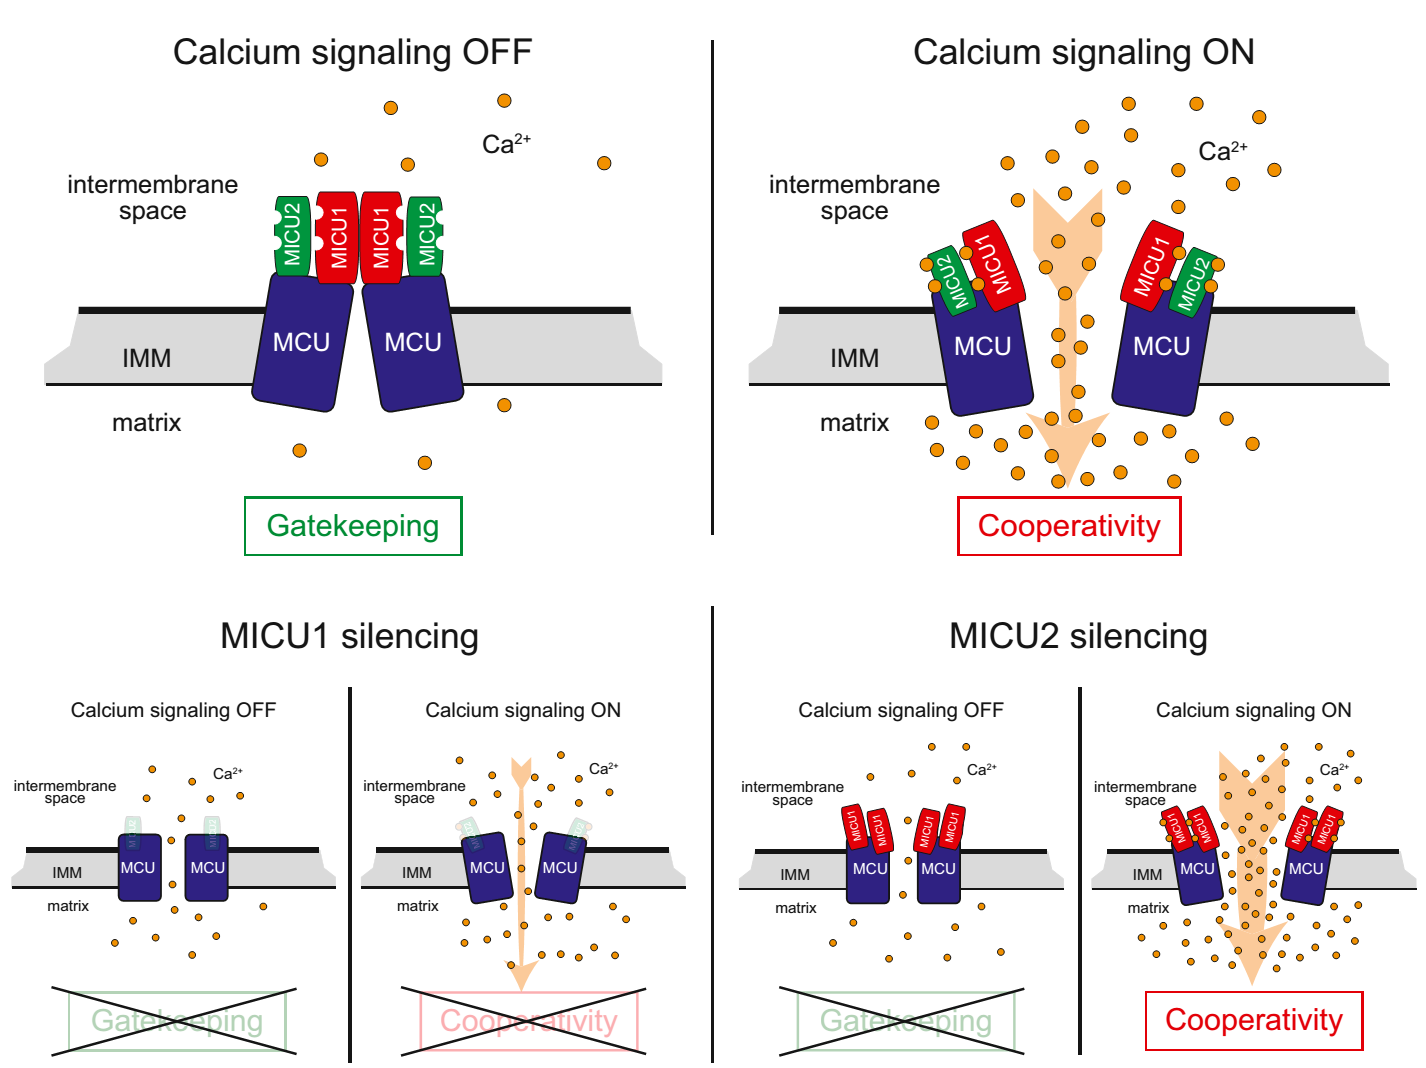
\includegraphics[width=0.95\textwidth]{rysunki/rozdzial_1/micu2control.png}
\caption[Proponowany model kontroli uniportera]{Proponowany model kontroli aktywności uniportera mitochondrialnego \cite{Patron2014}.}
\label{fig:micu2control}
\end{figure}

Doświadczenia Patron i współpracowników potwierdzają, że białka MICU1 i MICU2 znajdują się bardzo blisko siebie (w odległości nie większej niż 10 \AA). Znakowanie histochemiczne wykazało, że oba białka zajmują zbliżone lokalizacje w komórce (Ryc.~\ref{fig:micu2}, panel A). Dodatkowo wykonane przez nich doświadczenia z wykorzystaniem transferu energii F\''{u}rstera pomiędzy specjalnie skonstruowanymi białkami hybrydowymi obejmującymi MICU1 i MICU2 oraz ich połączenia z białkami fluorescencyjnymi GFP i~mCherry (\ref{fig:micu2}, panel B). Trawienie proteolityczne (Ryc.~\ref{fig:micu2}, panel C) wykazało, że monomer MICU1 ma masę molową 50 kDa, z kolei w kompleksie z MICU2 tworzą prążek na wysokości 95 kDa \cite{Patron2014}. 

\begin{figure}[ht]
	\centering
	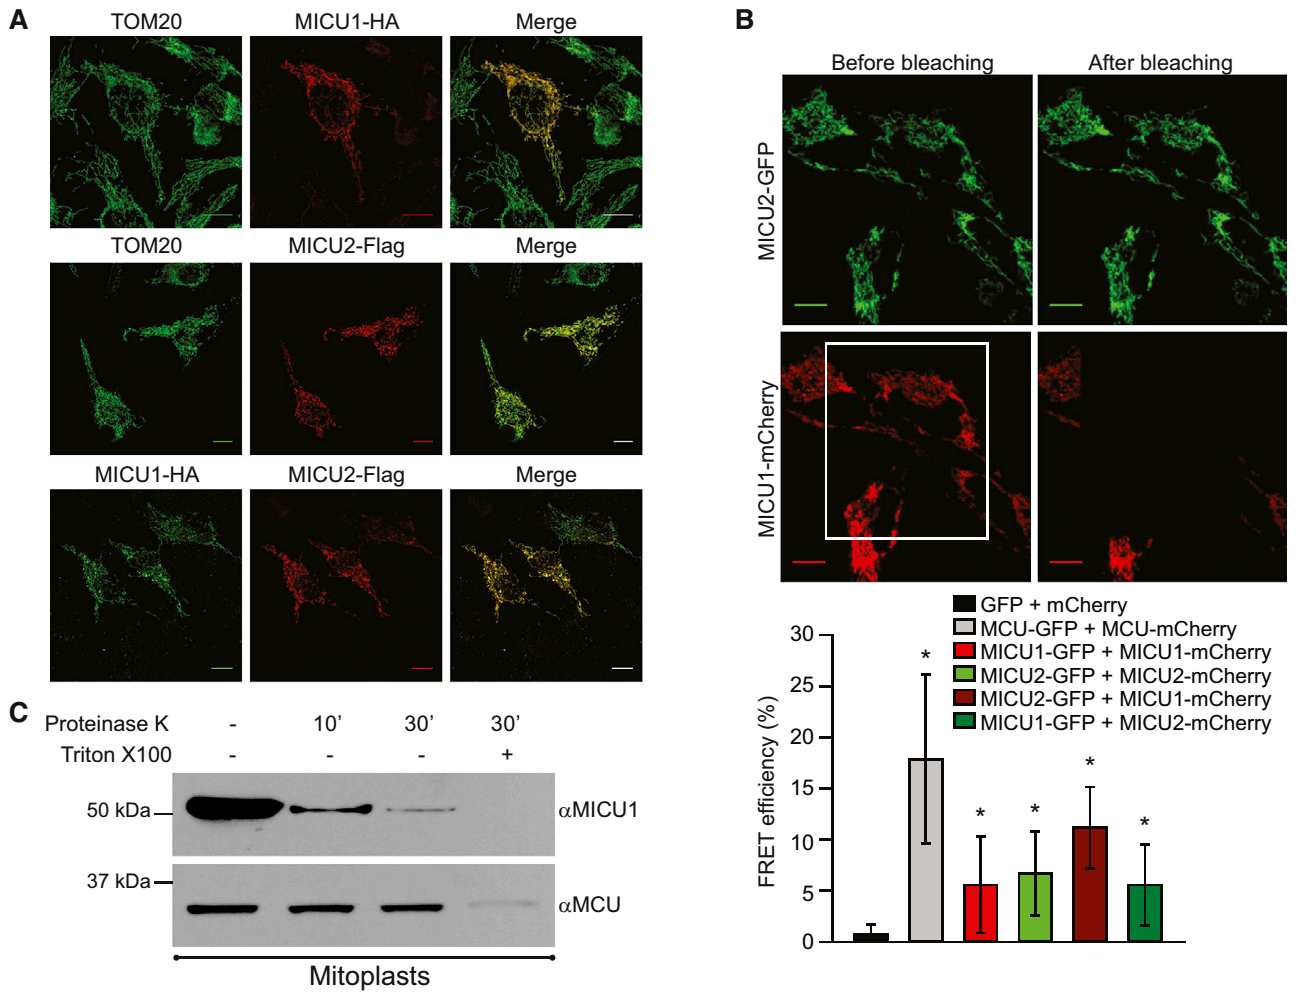
\includegraphics[width=1\textwidth]{rysunki/rozdzial_1/micu1micu2.png}
	\caption[Oddziaływanie pomiędzy MICU1 i MICU2]{Oddziaływania MICU1 i MICU2 w przestrzeni perymitochondrialnej. \textbf{(A)}: Komórki HeLa transfekowane były dwoma różnymi plazmidami, zawierającymi hybrydowe białka MICU-HA i/lub MICU2-Flag. Po 24. godzinach komórki były utrwalane i przeprowadzano barwienie histochemiczne z użyciem przeciwciał przeciwko fragmentom: $\alpha$HA, $alpha$Flag oraz przeciwko markerowi mitochondrialnemu $\alpha$Tom20. \textbf{(B)}: Analiza transferu energii FRET dla białek: MCU,MICU1, MICU2 transfekowanych GFP oraz mCherry. Poniżej zdjęcia z mikroskopu konfokalnego histogram oddziaływania między sobą poszczególnych par białek. \textbf{(C)} Delikatna proteoliza białek mitoplastów pozyskanych z wątroby myszy proteinazą K, znakowanych na obecność MICU1 (prążek 50 kDa) i MCU (prążek 37 kDa)~\cite{Patron2014}.}
	\label{fig:micu2}
\end{figure}

Kolejne mechanizmy kontroli aktywności obejmują wpływ nukleotydów adeninowychna kanał uniportera. Głównym czynnikiem aktywującym mitochondrialny uniporter wapniowy jest podwyższone stężenie Ca$^{2+}$ w cytozolu. Po akumulacji Ca$^{2+}$ w macierzy mitochondrialnej i powrocie do fizjologicznego stężenia Ca$^{2+}$ w cytozolu, aktywność uniportera obniża się. Allosteryczne oddziaływaniem jonów wapniowych reguluje aktywność MICU. Dla prawidłowego funkcjonowania uniportera wapniowego niezbędny jest również wysoki potencjał w poprzek błony mitochondrialnej. Ważnymi fizjologicznymi modulatorami aktywności uniportera wapniowego są nukleotydy adeninowe. Białko hamowane jest przez wysokie stężenie ATP, natomiast ADP stymuluje pobieranie wapnia do mitochondriów.

Prawdopodobnie oddziaływanie nukleotydów adeninowych z uniporterem wapniowym odbywa się za pośrednictwem mitochondrialnych receptorów purynergicznych: mP2y1, którego stymulacja prowadzi do zwiększenia aktywności uniportera i mP2y2, którego pobudzeniu towarzyszy hamowanie MCU. ADP może aktywować obydwa receptory, natomiast ATP jedynie mP2y2. W ten sposób szybkość pobierania wapnia do mitochondriów jest uzależniona od stosunku stężeń ATP/ADP w cytoplazmie. Endogennymi aktywatorami mitochondrialnego uniportera Ca$^{2+}$ są także poliaminy, a~przede wszystkim spermina. Związki te obniżają stężenie Ca$^{2+}$ wymagane do aktywacji uniportera. Również flawonoidy (kwercetyna, kempferol, genisteina i genistyna) aktywują MCU prawdopodobnie bezpośrednio oddziałując z uniporterem wapniowym.

W latach 90-tych zidentyfikowano kolejny mechanizm pobierania jonów wapniowych przez uniporter mitochondrialny. Mechanizm ten aktywny jest podczas krótkotrwałej ekspozycji mitochondriów na submikromolowe stężenie Ca$^{2+}$, które stanowią tzw. fizjologiczny puls wapniowy, związany z oscylacjami wapnia w komórce. Doświadczenia przeprowadzone przez Gunter i współpracowników oraz Vinogradow i Sparagna sugerują, że w tych warunkach mitochondria pobierają Ca$^{2+}$ znacznie wydajniej. Mechanizm został zdefiniowany jako tzw. szybki mechanizm pobierania jonów wapniowych \textbf{RaM} (ang. \textbf{ra}pid \textbf{m}ode of Ca$^{2+}$ uptake)\nomenclature{RaM}{szybki mechanizm pobierani jonów wapnia (ang. \textbf{ra}pid \textbf{m}ode of Ca$^{2+}$ uptake)} \cite{Buntinas2001,Gunter1990,Sparagna1995,Vinogradov1973}. Obecnie wiadomo już jest, że RaM realizowany jest przez uniporter, który może występować w kilku konformacjach charakteryzujących się różnym powinowactwem i przewodnictwem dla jonów wapnia.

\subsubsection{Mitochondrialny wymiennik Na$^+$/Ca$^{2+}$ (mNCX)}
\label{ch:mNCX}

Działanie mitochondrialnych transporterów drugiego rzędu, czyli mitochondrialnego wymiennika sodowo-wapniowego nie różni się od funkcjonowaniem od swojego cytoplazmatycznego odpowiednika (por. Rozdz.~\ref{ch:NCX}).

\bigskip

\subsubsection{Megakanał (PTP)}\label{ss:ptp}
Pod wpływem substancji osmotycznie czynnych, np. Ca$^{2+}$, mitochondria zwiększają objętość. Proces ten nazywany jest ,,pęcznieniem mitochondriów'' i może prowadzić do mechanicznego rozerwania błony wewnętrznej. Ponieważ wewnętrzna błona mitochondrialna posiada szereg wpukleń (tzw. grzebieni mitochondrialnych), jej powierzchnia jest kilkakrotnie większa od powierzchni błony zewnętrznej~\ref{app:b}. Uważa się, że za pęcznienie mitochondriów odpowiedzialny jest nieselektywny \textbf{megakanał PTP} (ang. \textbf{p}ermeability \textbf{t}ransition \textbf{p}ore) o średnicy 2.8 nm, którego aktywacja powoduje, że wewnętrzna błona mitochondriów staje się przepuszczalna dla molekuł o masie cząsteczkowej poniżej 1500 Da. to do pęcznienia mitochondriów, a nawet do mechanicznego rozerwania ich błony wewnętrznej.

Jedną z pierwszych zmian w mitochondriach jest powstanie i otwieranie się specyficznych porów mitochondrialnych określanych mianem PTP (por. Podrodz.~\ref{ss:ptp}). Powstają na styku zewnętrznej i wewnętrznej błony mitochondrialnej, a w ich skład wchodzą białka będące składnikami obu błon mitochondrialnych. Należą do nich m.in. należąca do IMM m.in. translokaza nukleotydów adeninowych -- ANT (ang. \textit{\textbf{a}denine \textbf{n}ucleotide \textbf{t}ranslocator}), która tworzy kompleks z białkiem VDAC i obwodowym receptorem benzodiazepiny - BPR\nomenclature{BPR}{obwodowy receptor benzodiazepiny (ang. \textit{\textbf{b}enzodiazepine \textbf{p}eripheral \textbf{r}eceptor})}, będących składnikami błony zewnętrznej. Model megakanału PTP przedstawiono schematycznie na Ryc.~\ref{fig:PTP}. W~strukturze poru zidentyfikowano również szereg enzymów, np. kinaza kreatynowa. Jony wapniowe stanowią istotny czynnik aktywujący megakanał w układach doświadczalnych, natomiast w~komórce, oprócz Ca$^{2+}$ na modulację aktywności megakanału mogą wpływać również białka z rodziny Bcl-2/Bax oraz obecność związków związanych z metabolizmem lipidów takich jak ceramid i kwas arachidonowy.

\begin{figure}[tb]
\centering
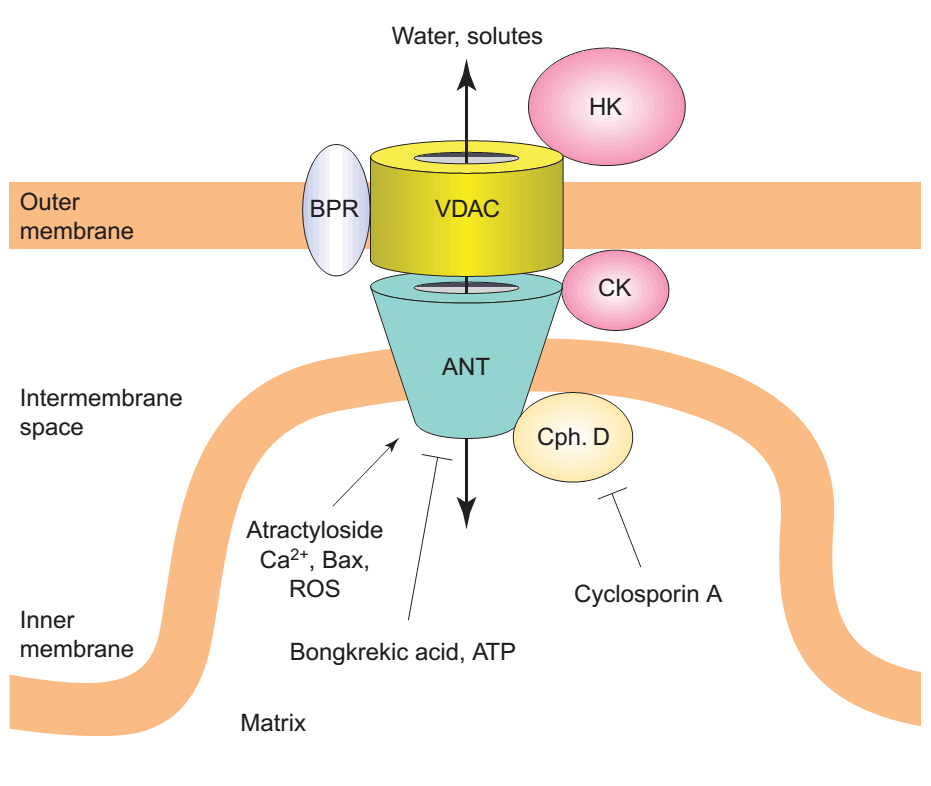
\includegraphics[width=0.85\textwidth]{rysunki/rozdzial_1/ptp.png}
\caption[Megakanał PTP]{Strukturalne przedstawienie megakanału PTP. Przy otwarciu kanału woda i rozpuszczone w niej substancje wnikają do macierzy, powodując zwiększenie jej objętości. \textbf{ANT} - translokaza nukleotydów adeninowych, \textbf{BPR} - obwodowy receptor benzodiazepiny; \textbf{CK} - kinaza kreatyninowa; \textbf{CL-S} - syntaza kardiolipiny; \textbf{HSD/I} - dehydrogenaza/izomeraza 3$\beta$=hydroksysteroidów; \textbf{GK} - kinaza glicerolowa; - peroksydaza glutationowa; \textbf{HK} - heksokinaza; \textbf{VDAC} - poryna; Na schemacie uwzględniono również miejsca działania niektórych aktywatorów (atraktylozyd, Bax, Ca$^{2+}$, ROS) i~inhibitorów (cyklosporyna A, kwas bongkrekowy (BA), ATP) otwarcia kanału \cite{Leo2005}.}
\label{fig:PTP}
\end{figure}

\section{Kompleksy błonowe}\label{s:kompleksy_blonowe}

Komórka jest struktura dynamiczną. Tysiące procesów biochemicznych zachodzących w~bardzo małej przestrzeni możliwe jest dzięki kompartmentalizacji. Cytozol podzielony jest na mniejsze przedziały, dzięki czemu blisko siebie mogą zachodzić wykluczające się procesy biochemiczne lub składowane są produkty tych przemian. Kompartmenty różnych rodzajów mogą się ze sobą łączyć w odpowiedzi na stan fizjologiczny komórki lub w wyniku aktywacji szlaku sygnałowego. Sytuacja taka ma miejsce np. w~przypadku sygnalizacji wapniowej. Większość dużych organelli jest w~stanie magazynować wapń: retikulum, mitochondria, aparat Golgiego \cite{Micaroni2012}, jądro komórkowe\cite{Alonso2006}, czy drobne pęcherzyki - mikrosomy \cite{Neher1998}. Większość tych struktur może oddziaływać ze sobą w~sposób bezpośredni, tworząc \textbf{kompleksy błonowe}. Pozwala to na szybkie i~efektywne przekazywanie sygnałów i integrację różnych szlaków sygnałowych \cite{Laude2009,Petersen2002}. Miejsca kontaktu określane są również jako mikrodomeny \cite{Berridge2006,Rizzuto2006}. Są to wyizolowane przestrzenie, gdzie stężenie wapnia może zwiększyć się kilkunastokrotnie w bardzo krótkim czasie. W zależności od organelli wchodzących ze sobą w~interakcje wyróżnia się szereg mikrodomen. Niektóre tworzone \textit{,,ad hoc"} w~wyniku aktywacji szlaku sygnałowego, inne z kolei będące stałym elementem szlaku, tworzone konstytutywnie.


Połączenie błony retikulum z błoną komórkową pozwala na szybkie uzupełnienie jonów wapnia w ER z puli zewnątrzkomórkowej. Podobnie mitochondria mogą łączyć się zarówno z ER, jak i błoną komórkową, kształtując dynamikę sygnału wapniowego w komórce \cite{Hayashi2009}. Najważniejszymi przedziałami, które uczestniczą w sygnalizacji wapniowej są mitochondria i~siateczka śródplazmatyczna (Ryc.~\ref{fig:mitoER}). Struktury te ściśle współpracują ze sobą, tworząc fizyczne połączenia przypominające synapsy, umożliwiające bezpośrednie przekazywanie sygnału z jednego kompartmentu do drugiego. Struktury takie nazywane są kompleksami błonowymi. Kompleks powstający na styku mitochondria-ER określany jest jako \textbf{kompleksy błon związanych z mitochondriami - MAM} (ang. \textit{\textbf{m}itochondria \textbf{a}ssociated \textbf{m}embranes})\nomenclature{MAM}{błony związane z mitochondriami (ang. \textit{\textbf{m}itochondria \textbf{a}ssociated \textbf{m}embranes})}. Szacuje się, że większość jonów wapniowych uwolnionych z ER buforowana jest w mitochondriach~\cite{Marhl2000}. Aktywacja kanałów IP$_3$R może spowodować wzrost stężenia jonów wapnia w przestrzeni mitochondrialnej, przekraczającego nawet $\approx$20 krotnie globalne wzrosty jonów wapnia wywołanych aktywacją tych receptorów~\cite{Csordas1999}. Zaobserwowano też, że wzrost stężenia jonów wapnia w cytozolu indukowany aktywacją receptorów IP$_3$R, powoduje odpowiadający mu wzrost stężenia jonów wapnia w matriks \cite{Rizzuto2006}. Dodatkowo badania mikroskopowe potwierdzają, że większość mitochondriów (80\%) jest połączona z retikulum endoplazmatycznym \cite{Mannella1998}. Ostateczne Csord\'{a}s i współpracownicy wykazali, że miejsca uwalniania jonów wapniowych z retikulum (obecność receptora IP$_3$R) powiązane są z obszarami występowania uniportera mitochondrialnego, odpowiedzialnego za transport jonów wapniowych do matriks. \cite{Csordas1999}

\subsection{MAM}\label{ss:MAM}

Istnienie kompleksów błonowych, które wyróżniały się obecnością enzymów charakterystycznych dla frakcji retikularnej i mitochondrialnej zostało odkryte już w latach 70-tych. W swoje pracy Dennis i Kennedy wyizolowali ze szczurzych hepatocytów specyficzny rodzaj frakcji błonowej, którą określili jako ,,frakcja x'' \cite{Dennis1972}. Intensywne badania tej frakcji rozpoczęły się dopiero 20 lat później, kiedy to powiązano frakcję x~z~intensyfikacją metabolizmu lipidów \cite{Rusinol1994}. ,,Frakcja x'' to kompleks błon siateczki śródplazmatycznej i mitochondrium, które łączą się w przypominający synapsą interfejs spajający te dwa organella (schemat przedstawiony został na Ryc.~\ref{fig:MAMschemat}).

\begin{figure}[!ht]
  \centering
  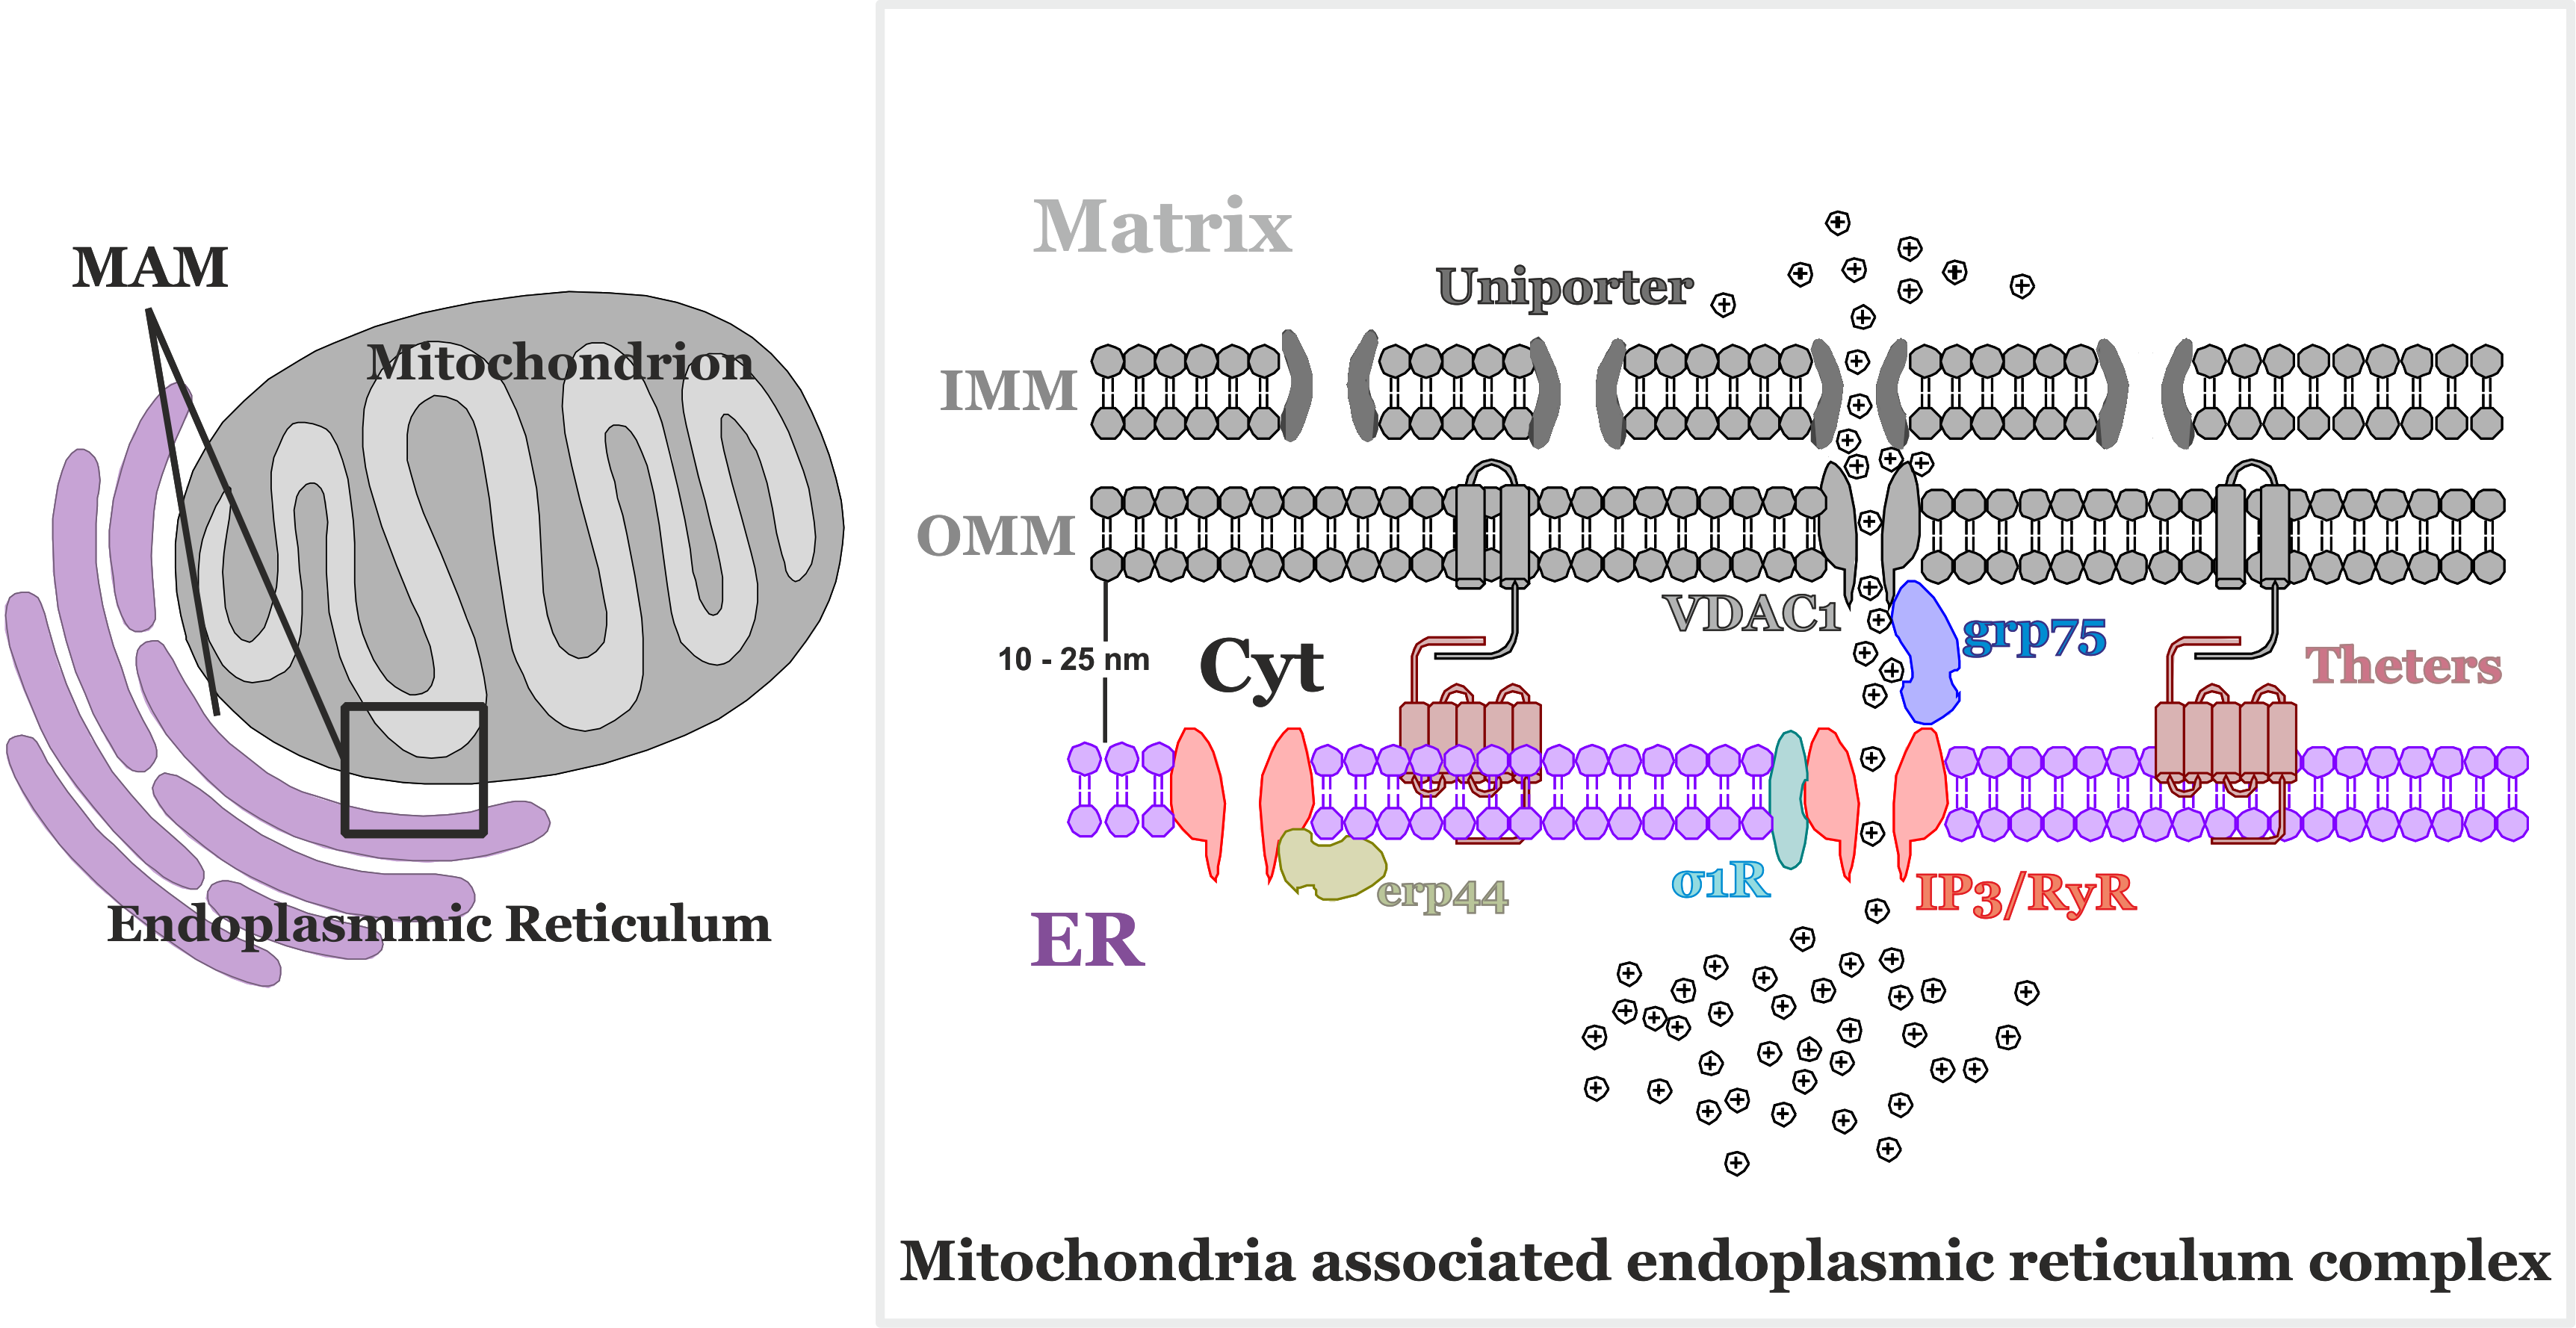
\includegraphics[width=1\textwidth]{rysunki/rozdzial_1/MAM}
  \caption[MAM - kompleks mitochondrialno-retikularny, schemat]{Kompleks mitochondrialno-retikularny (MAM), ER - siateczka śródplazmatyczna, Cyt - cytozol, IP$_3$R/RyR - kanały wapniowe na powierzchni ER, \mbox {VDAC-1/uniporter} - kanały wapniowe mitochondrium; białka stabilizujące połączenie: erp44/erp57 - białka siateczki śródplazmatycznej 44/57, $\sigma_1$R - \mbox {sigma-1 receptor} oraz chaperon grp75 \cite{Dyzma2012,Szopa2013}.}
  \label{fig:MAMschemat}
\end{figure}


Odległość między błonami kompleksu waha się od 9 nm dla gładkiej siateczki śródplazmatycznej, do 30 nm w przypadku szorstkiej \cite{Csordas2006}. Interfejs mitochondrialno-retikularny stabilizowany jest przez szereg protein, które w większości powiązane są z głównymi elementami przewodzącymi sygnał wapniowy w tych kompartmentach, tj. receptorem IP$_3$, pompą wapniową SERCA oraz kanałem VDAC~(Tab. \ref{tab:MAMproteins}, Ryc.~\ref{fig:MAMschemat}). Jak już wspomniano, struktury te mogą powstawać ,,\textit{de novo}'' w trakcie aktywacji szlaku sygnalizacji wapniowej \cite{Csordas2010}.


Błony białkowo-lipidowe pozostają ze sobą połączone nawet podczas ekstrakcji opartej na frakcjonowaniu komórek za pomocą wirowania \cite{Wieckowski2009}. Struktury te widoczne są na mikrografii z mikroskopu elektronowego - Ryc.~\ref{fig:MAMelectro1} \cite{Pereda1992} oraz Ryc.~\ref{fig:MAMelectro3} \cite{Lebiedzinska2009,Scheffler1999}, jak i mikrografiach uzyskanych za pomocą tomografii elektronowej - Ryc.~\ref{fig:MAMfoto2} \cite{Rowland2012}.

\begin{figure}[!ht]
  \centering
  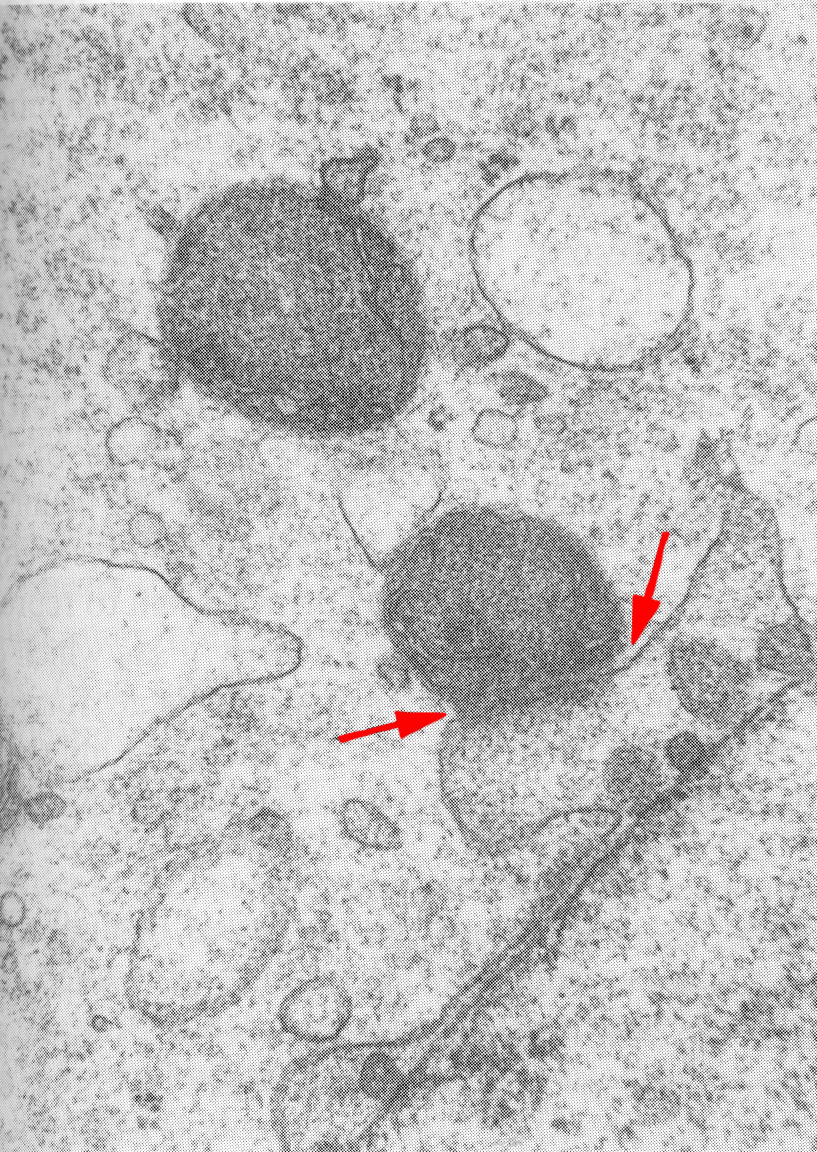
\includegraphics[width=0.65\textwidth,angle=90]{rysunki/rozdzial_1/MAM_electro_1}
  \caption[Miejsca kontaktu mito-ER w blastomerach człowieka]{Mikrografia wykonana transmisyjnym mikroskopem elektronowym z blastomeru (czterokomórkowy embrion \emph{in vitro}). Strzałki wskazują miejsca bliskiego kontaktu mitochondrium z~wypukleniami pochodzącymi z otoczki jądrowej, które następnie przechodzą w struktury retikularne (powiększenie x40000)~\cite{Pereda1992}.}
  \label{fig:MAMelectro1}
\end{figure}


\begin{sidewaysfigure}[!!ht]
  \centering
  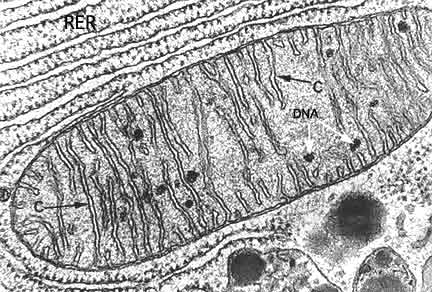
\includegraphics[width=0.545\textwidth]{rysunki/rozdzial_1/mitochon_ER}
  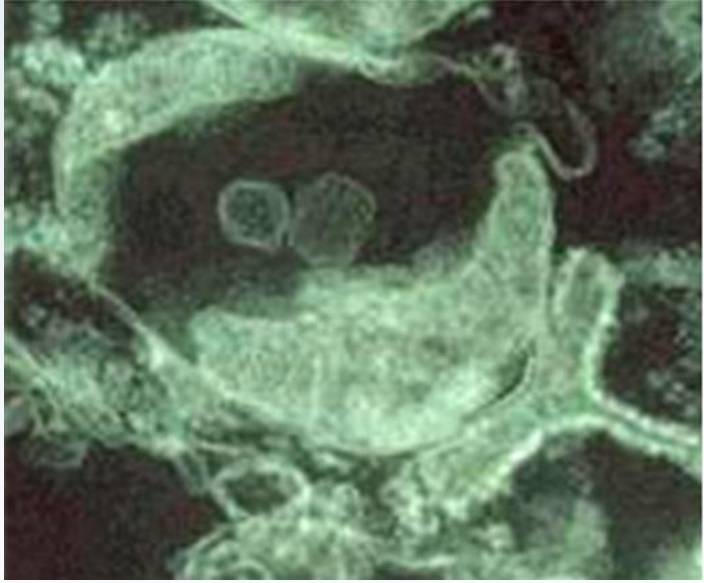
\includegraphics[width=0.45\textwidth]{rysunki/rozdzial_1/MAM_picture1}
  \caption[Miejsca kontaktu mito-ER w komórce]{Miejsca kontaktu mito-ER w komórce. Prawy panel - mikrografia z mikroskopu elektronowego autorstwa R. Więckowskiego -powiększenie $\times$26000~\cite{Lebiedzinska2009}. Lewy panel - mikrografia przedstawiająca ułożenie mitochondrium i szorstkiej siateczki śródplazmatycznej (RER) na podstawie ~\cite{Scheffler1999}. Strzałki wskazują grzebienie mitochondrialne (\textbf{C}).}
  \label{fig:MAMelectro3}
\end{sidewaysfigure}


\begin{table}[!ht]
  \centering
  \begin{tabular}{lp{9cm}r}
    \toprule[0.12em]
    \textbf{Białko} & \textbf{Funkcja} & \textbf{Referencje} \\ \midrule[0.06em]
    \ngray \multicolumn{3}{c}{\textbf{Siateczka śródplazmatyczna}}\rule[-2ex]{0pt}{5.5ex} \\
    \rule[-2ex]{0pt}{5.5ex} IP$_3$R1-3/RyR & kanały wapniowe w ER & \cite{Hayashi2009} \\
    \rule[-2ex]{0pt}{5.5ex} BiP & chaperon ER  & \cite{Gething1999} \\
    \rule[-2ex]{0pt}{5.5ex} Sigma1-R  & reguluje funkcjonowanie IP$_3$R1 & \cite{Hayashi2007,Szabadkai2006} \\
    \rule[-2ex]{0pt}{5.5ex} FKBP12  & reguluje funkcjonowanie kanałów RyR & \cite{Chelu2004}   \\
    \rule[-2ex]{0pt}{5.5ex}ERp44   & reguluje funkcjonowanie IP$_3$R3   & \cite{Szabadkai2006} \\
    \rule[-2ex]{0pt}{5.5ex} ERp57  & białko związane z Ca$^{2+}$-ATP-azą  & \cite{Szabadkai2006} \\
    \rule[-2ex]{0pt}{5.5ex}SERCA  & pompa wapniowa membrany ER  & \\
    \rule[-2ex]{0pt}{5.5ex} kalretikulina & bufor wapniowy  & \cite{Szabadkai2006} \\
    \rule[-2ex]{0pt}{5.5ex} kalneksyna  & bufor wapniowy  & \cite{Szabadkai2006} \\
    \ngray \multicolumn{3}{c}{\textbf{Cytozol}}\rule[-2ex]{0pt}{5.5ex} \\
    \rule[-2ex]{0pt}{5.5ex} PACS-2  & kontroluje połączenia ER-Mit i apoptozę wywołaną białkiem Bid \nomenclature{PACS}{ang. \textit{\textbf{p}hosphofurin \textbf{a}cidic \textbf{c}luster \textbf{s}orting protein}}  & \cite{Simmen2005} \\
    \rule[-2ex]{0pt}{5.5ex} AMF-R (i.e gp78) & pomaga w stabilizacji MAM - rekrutuje p97 & \cite{Wang2000}\\
    \rule[-2ex]{0pt}{5.5ex} S100A1 & reguluje napływ Ca$^{2+}$ do ER& \cite{Volkers2010} \\
    \rule[-2ex]{0pt}{5.5ex} S100B   & białko spinające membrany, bierze udział w transporcie lipidów & \cite{Wen2012} \\
    \rule[-2ex]{0pt}{5.5ex} grp75   & białko powiązane z VDAC  & \cite{DeBrito2010,Szabadkai2006} \\
    \rule[-2ex]{0pt}{5.5ex} hsp60   & białko szoku cieplnego, stabilizator połączenia & \cite{Szabadkai2006}  \\
    \rule[-2ex]{0pt}{5.5ex}Mitofuzyna-2& spina ER z mitochondrium  & \cite{DeBrito2008,Merkwirth2008} \\[0.1cm]
    \ngray \multicolumn{3}{c}{\textbf{Mitochondria}}\rule[-2ex]{0pt}{5.5ex} \\
    \rule[-2ex]{0pt}{5.5ex} VDAC-1   & kanał Ca$^{2+}$ na OMM   & \cite{Hayashi2009,Hayashi2007} \rule[-2ex]{0pt}{5.5ex} \\
    \rule[-2ex]{0pt}{5.5ex} Uniporter & kanał dla Ca$^{2+}$ na IMM & \cite{Hayashi2007,Hayashi2009} \\[0.1cm] \bottomrule[0.12em]
  \end{tabular}
  \caption{Najważniejsze białka tworzące kompleksy MAM.}
  \label{tab:MAMproteins}
\end{table}

\FloatBarrier

Według \cite{Rowland2012}, połączenia pomiędzy retikulum endoplazmatycznym, a mitochondriami obserwowane są w wielu typach komórek należących do różnych gromad organizmów żywych: w komórkach drożdży, linii komórkowej DT40 kurzych limfocytów, hepatocytach szura (Ryc.~\ref{fig:MAMfoto2}, A-C) i zdefiniowane są tam jako obszary, w których błony obu organelli zbliżone są do siebie, ale nie zlewają się,a odległość między nimi wynosi 10--30 nm. Niewielka odległość pomiędzy błonami pośrednio sugeruje, że mogą być one spinane ze sobą za pomocą białek zlokalizowanych na powierzchni przeciwległych błon (\ref{fig:MAMfoto2}, C). Ponadto z tego powodu w miejscach kontaktu problematyczna wydaje się lokalizacja rybosomów w przypadku RER. Z obserwacji dokonanych przy użyciu tomografii elektronowej wynika, że miejsca kontaktu mogą przybierać bardzo różnorodne formy, od niewielkich ,,łat'', po pierścienie ER otaczających podłużne mitochondria. Wydaje się też, że połączenia MAM są stosunkowo stabilne i nawet gdy jedno z organelli porusza się, drugie podąża wraz z nim, nie zrywając kontaktu. (\ref{fig:MAMfoto2}, Ea-Eb). Jak wynika z obserwacji żywych komórek, połączenia mitochondriów i ER nie wpływają na rozmieszczenie tych organelli w komórce (\ref{fig:MAMfoto2}, D).



\begin{figure}[ht]
  \centering
  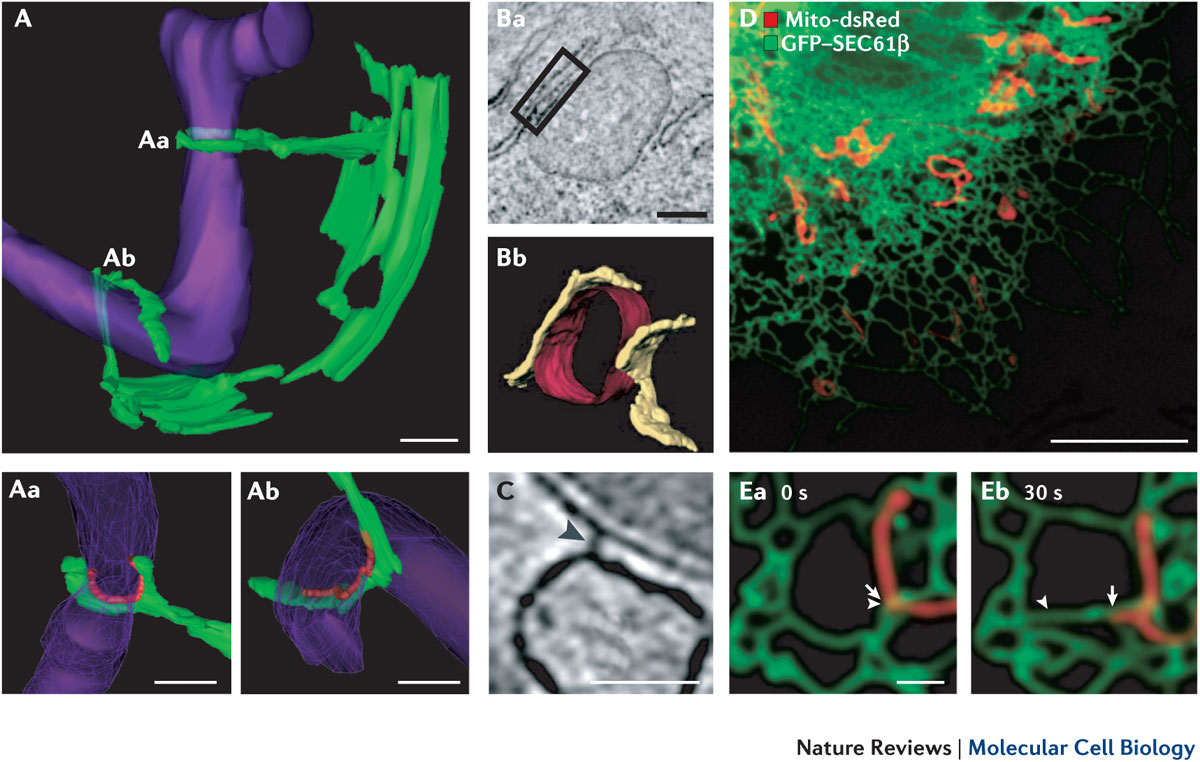
\includegraphics[width=1\textwidth]{rysunki/rozdzial_1/MAM_picture2}
  \caption[MAM - mikrografia z tomografii elektronowej]{\textbf{A)} Trójwymiarowe obrazy połączeń mitochondriów z ER, uzyskane za pomocą tomografii elektronowej, ukazane w powiększeniu na panelach Aa oraz Ab. ER kolor zielony, mitochondrium kolor fioletowy w komórkach drożdży. \textbf{B)} Mikrografia połączeń mitochondrium (kolor czerwony) oraz ER (kolor żółty) z tomografii cryo-EM (Ba) i zbudowany na jej podstawie model 3-D (Bb) w komórkach kurzych z~linii DT40 z dezaktywowanym genem \textit{ip3r}. \textbf{C)} Tomografia elektronowa hepatocytów szczura, ukazujących w powiększeniu elementy spinające (theters) ER i mitochondria. \textbf{D)} Barwienie przyżyciowe za pomocą białek fluorescencyjnych: dsRED (znakuje mitochondria na czerwono) oraz GFP (pokazuje retikulum endoplazmatyczne, a dokładnie kompleks transportujący Sec61$\beta$, na zielono). \textbf{E)} powiększone miejsce kontaktu z panelu D, w~dwóch krokach czasowych (0 i 30 sekund) wskazują, że ER porusza się wraz z~mitochondrium. Znacznik odległości dla \textbf{A} wynosi 200nm, \textbf{B} wynosi 250nm, \textbf{C}~wynosi 50nm, \textbf{D} wynosi~10$\mu$m oraz \textbf{E} wynosi 1 $\mu$m~\cite{Rowland2012}.}
  \label{fig:MAMfoto2}
\end{figure}

Szczególną rolę w procesie ustawienia kanałów jonowych w apozycji odgrywają specjalne białka spinające, wzmacniające połączenia mitochondrium-ER (w dalszej części akapitu nazywane połączeniami Mit-ER) i odgrywające olbrzymia rolę w~przepływie wapnia między tymi organellami. W jednym z doświadczeń Csord\'{a}s i współpracownicy wykazali, że kontrola przepływu jonów wapniowych z~ER do mitochondrium może odbywać się nie tylko poprzez regulację pracy kanałów białkowych, ale także poprzez odpowiednią kontrolę odległości i stabilizację połączenia w~interfejsie MAM \cite{Csordas2006}. Aby zbadać wpływ stabilności połączeń na transmisję Ca$^{2+}$ autorzy zaczęli od wykorzystania tomografii elektronowej do obserwacji izolatów mitochondriów z wątroby szczura i~szczegółowego uwidocznienia połączeń Mit--ER z bardzo dużą rozdzielczością. W sekcji A Ryc.~\ref{fig:MAMfoto3} widać cienkie struktury łączące pęcherzyki ER z~OMM (powiększone na panelach 1, 2 i 3). Widoczne struktury spinające występują w klastrach po 6 i więcej, rozciągając się na długości 13--22 nm. Odległość pomiędzy powierzchniami błon wynosi 6--15 nm. Autorzy obserwowali również podobne struktury w nieuszkodzonych hepatocytach szczura i linii komórkowej DT40 uzyskanej z kurzych limfocytów B, zarówno w~przypadku gładkiej, jak i szorstkiej siateczki śródplazmatycznej, jednak z powodu większego ,,zagęszczenia'' ośrodków w nieuszkodzonych komórkach były one o wiele słabiej widoczne (Ryc.~\ref{fig:MAMelectro3}, B). Obserwacje wskazują, że struktury spinające w przypadku gładkiej siateczki śródplazmatycznej mają średnią długość 9--16 nm, natomiast w przypadku szorstkiej siateczki śródplazmatycznej minimum 19--30 nm. Dlatego też w pracy tej autorzy sugerują, iż zróżnicowanie odległości między organellami może być jednym z mechanizmów kontroli propagacji sygnału wapniowego z ER do mitochondrium.

\begin{figure}[ht]
\centering
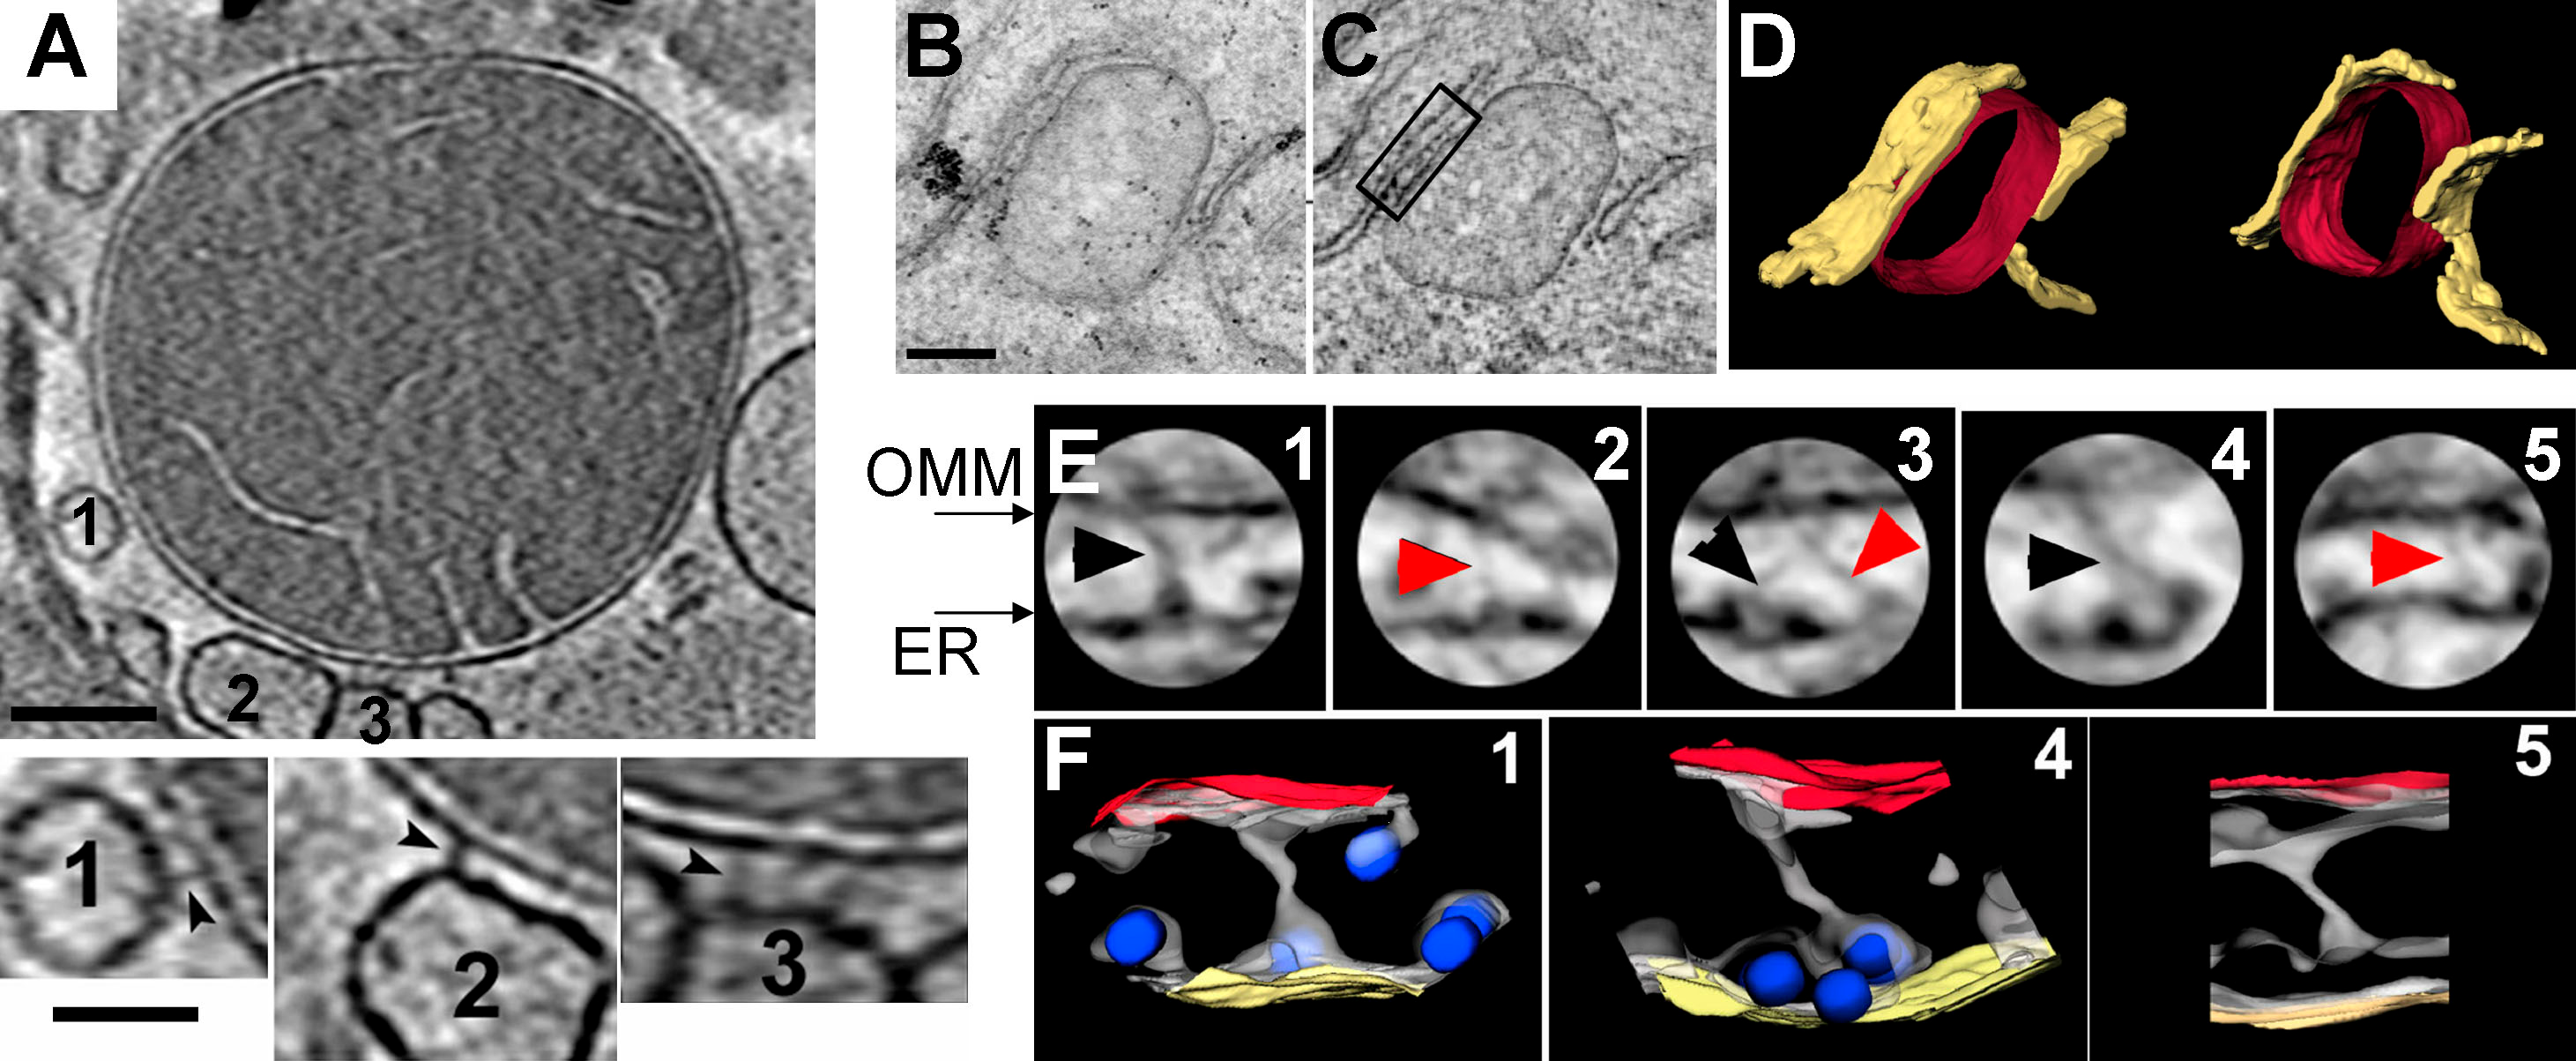
\includegraphics[width=1\textwidth]{rysunki/rozdzial_1/MAMfoto3.png}
\caption[MAM - kompleks mitochondrialno-retikularny, białka spinające]{\textbf{A)} Mikrografie cry-ET izolatów mitochondriów z hepatocytów szczura, ukazujących szereg połączonych pęcherzyków z mitochondriami (znacznik odległości 100 nm), pokazanych w powiększeniu na dolnych panelach A (znacznik odległości 50 nm). \textbf{B,C)} mikrografie kurzych komórek DT40, pokazujących połączenie Mito-ER. \textbf{D)} trójwymiarowy model połączenia, gdzie ER oznaczono kolorem żółtym, natomiast mitochondria kolorem czerwonym. \textbf{E)} skany obszaru kontaktu o średnicy 130 nm z~zaznaczonymi strukturami spinającymi (kolorem czarnym wyróżniono struktury spinające kończące się na rybosomach). \textbf{F)} modele regionów prezentowanych na panelach w sekcji \textbf{E}. OMM kolorowane na czerwono, ER na żółto, struktury spinające na szaro. Rybosomy oznaczono kolorem niebieskim~\cite{Csordas2006}.}
\label{fig:MAMfoto3}
\end{figure}

W celu osłabienia połączeń Mit--ER, Csord\'{a}s i współpracownicy \cite{Csordas2006} zastosowali ograniczoną proteolizę. Badanie uwalniania jonów wapnia z kanałów IP$_3$R w komórkach poddanych wcześniej ograniczonej proteolizie, wykazały że proteoliza wpływa na poziom akumulacji jonów wapniowych w mitochondriach. W grupie kontrolnej podanie 8 $\mu$M IP$_3$ powodował wyrzut jonów wapnia z ER do cytozolu, co skutkowało wzrostem stężenia tych jonów w mitochondriach. Po zastosowaniu enzymu proteolitycznego - proteinazy K - wyrzut jonów wapnia z ER nie powodował wzrostu stężenia jonów wapnia w mitochondriach \cite{Csordas2006}.

\begin{figure}[ht]
\centering
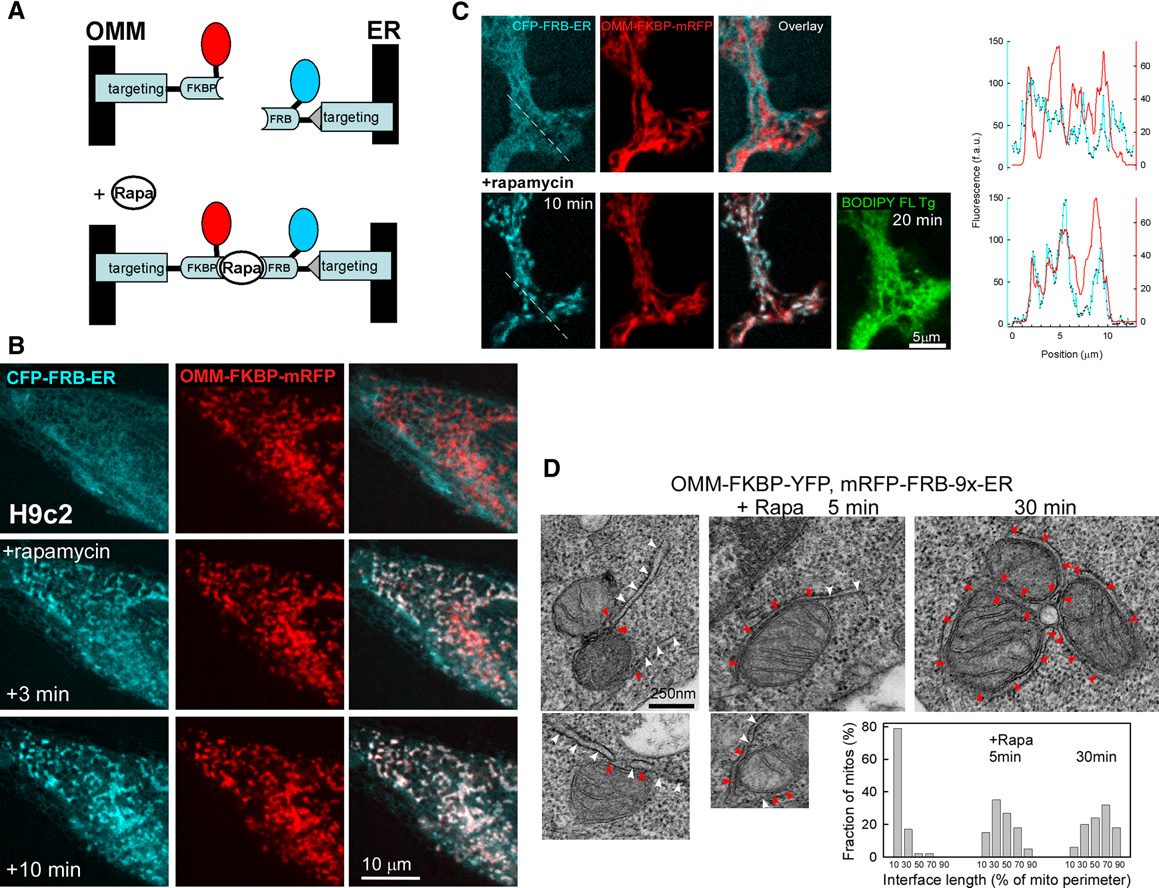
\includegraphics[width=0.9\textwidth]{rysunki/rozdzial_1/rapa.png}
\caption[Struktury spinające kompleksy mitochondrialno-retikularne]{Schemat opisujący eksperyment ukazujący połączenia powstające pomiędzy zewnętrzną błoną mitochondrialną (OMM) oraz błona ER. (\textbf{A}) Zdjęcie ilustrujący indukowane rapamycyną mostki białkowe. (\textbf{B}) Zdjęcia wykonane pod mikroskopem konfokalnym, ukazujące pojedyncze komórki RBL-2H3 ze wzbudzoną nadekspresją mostków OMM-ER, ukazujące rozmieszczenie powiązanych z nimi barwników 1, 3 oraz 15 minut po potraktowaniu 100 nM roztworem rapamycyny. (\textbf{C}) Zdjęcia spod mikroskopu konfokalnego komórek H9c2 z wywołana nadekspresją mostków OMM-ER, przed i po 10 minutach ekspozycji na rapamycynę (100nM) \cite{Csordas2010}.}
\label{fig:rapamycin}
\end{figure}

Dodatkowo w \cite{Csordas2010} Csord\'{a}s i współpracownicy zsyntetyzowali indukowane rapamycyna sztuczne miejsca połączeń ER-mitochondrium (Ryc.~\ref{fig:rapamycin}). Doświadczenie polegało na uzyskaniu mutantów linii komórek RBL-2H3, z~genami białek hybrydowych, które symulowały obecność protein spinających na powierzchni ER i mitochondrium - tzw. linkery ER-OMM. Jedno z białek fuzyjnych składało się z fragmentu białka AKAP1 (ang. \textit{\textbf{A}-\textbf{k}inase \textbf{a}nchor \textbf{p}rotein \textbf{1}})\nomenclature{AKAP1}{ang. \textit{\textbf{A}-\textbf{k}inase \textbf{a}nchor \textbf{p}rotein \textbf{1}}}, który stanowiła jego sekwencja sygnałowa (reszty od 34-63), kierująca białko do OMM i białka wiążącego rapamycynę (FKBP12) z czerwonym białkiem fluorescencyjnym (mRFP1 - ang. \textit{\textbf{m}itochondrial \textbf{r}ed \textbf{f}luorescent \textbf{p}rotein 1})\nomenclature{mRFP1}{czerwone białko fluorescencyjne (ang. \textit{\textbf{m}itochondrial \textbf{r}ed \textbf{f}luorescent \textbf{p}rotein 1})}. Drugie białko fuzyjne skierowane było z kolei do ER i składało się z: sekwencji kierunkowej do ER (wziętej z białka SAC1), białka wiążącego rapamycynę (FRB) oraz niebieskiego białka fluorescencyjnego (CFP - ang. \textit{\textbf{c}yan \textbf{f}luorescent \textbf{p}rotein})\nomenclature{CFP}{niebieskie białko fluorescencyjne (ang. \textit{\textbf{c}yan \textbf{f}luorescent \textbf{p}rotein})} \cite{Csordas2010}. Podanie rapamycyny powodowało dimeryzacje białek FKBP12 i FRB, co ,,zszywało'' ze sobą błony ER i OMM, zbliżając je znacznie do siebie. W publikacji autorzy nie ograniczyli się jedynie do wizualizacji połączeń między ER i mitochondriami. Konstruując kolejne białka, które łączyły linkery ER-OMM z~,,ratiometric-pericam'' uzyskali białko pomostowe, wrażliwe na obecność jonów wapnia, czyli most OMM-pericam-FKBP-FRB-ER, który pozwalał na pomiar stężenia jonów wapnia w interfejsie ER-OMM.

%\begin{figure}[ht]
%\centering
%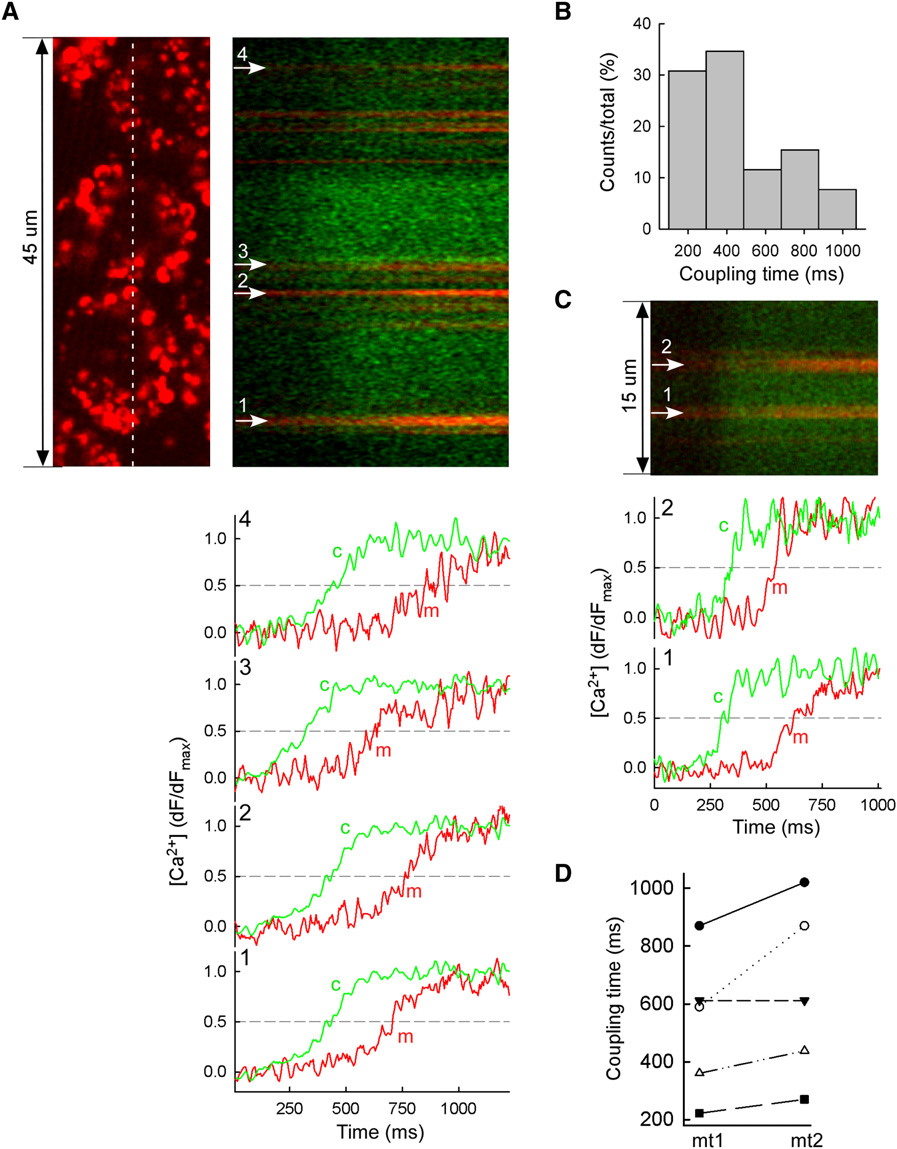
\includegraphics[width=0.9\textwidth]{rysunki/rozdzial_1/er_omm_ca.png}
%\caption[Pomiar stężenia Ca$^{2+}$ w MAM]{Pomiar stężenia Ca$^{2+}$ w MAM}
%\label{fig:caMAMmeasurement}
%\end{figure}

\FloatBarrier
\subsection{PAM}


Uwalnianie jonów wapnia z ER do cytoplazmy prowadzi do częściowego opróżnienia magazynów wapniowych w świetle siateczki śródplazmatycznej. Spadek stężenia jonów wapnia w~ER aktywuje napływ Ca$^{2+}$ ze środowiska zewnątrzkomórkowego do cytoplazmy poprzez zlokalizowane w błonie komórkowej kanały wapniowe typu \mbox{SOCEC} (ang. \textbf{s}tore \textbf{o}perated \textbf{c}alcium \textbf{c}hannel), zapewniające przepływ jonów określany mianem \textbf{CRAC} (ang. Ca$^{2+}$ Release Activated Ca$^{2+}$ Current). Wprowadzone w ten sposób do komórki jony wapnia mogą zostać wykorzystane do uzupełnienia magazynów wapniowych w świetle ER, na drodze aktywności ATPazy SERCA. Zjawisko to określa się mianem pojemnościowego napływu jonów wapniowych lub napływu regulowanego przez magazyny wapniowe (CCE/SOCE, ang. \textbf{c}apacitative \textbf{c}alcium \textbf{e}ntry/\textbf{s}tore \textbf{o}perated \textbf{c}alcium \textbf{e}ntry). Sposób, w jaki funkcjonalnie powiązane są ze sobą magazyny wapniowe w ER z kanałami SOC w błonie komórkowej jest w ostatnich latach przedmiotem intensywnych badań. Momentem przełomowym owych studiów było niedawne odkrycie, że białka \textbf{STIM1} i \textbf{Orai1/CRACM1} są niezbędne dla przebiegu SOCE, co wykazano stosując m.in. technikę interferencji RNA. Co więcej, naturalnie występująca w białku Orai1 mutacja R91W prowadzi do zniesienia CCE w limfocytach T, co klinicznie manifestuje się ciężkim, złożonym niedoborem odporności (SCID, ang. \textbf{s}evere \textbf{c}ombined \textbf{i}mmunodeficiency). Wykazano również, że równoczesna nadekspresja białek STIM1 i Orai1 prowadzi do znacznego nasilenia pojemnościowego napływu wapnia.

\begin{figure}[tb]
	\centering
	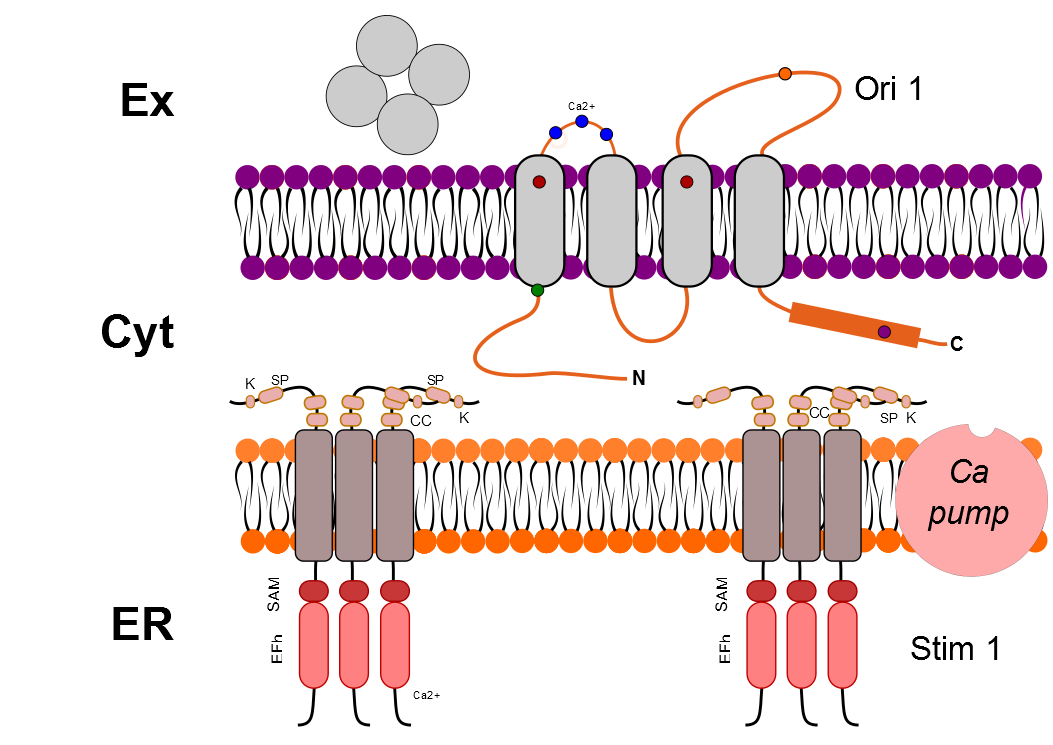
\includegraphics[width=0.9\textwidth]{rysunki/rozdzial_1/PAM.png}
	\caption [PAM - kompleks białkowy]{PAM - kompleks białkowy, przez który odbywa się pojemnościowy napływ wapnia. \textbf{Ex} - środowisko zewnątrzkomórkowe; \textbf{Cyt} - cytozol; \textbf{ER} - retikulum endoplazmatyczne. \textbf{EFh} - domeny EF-hand.}
	\label{fig:PAM}
\end{figure}

Orai1 to zlokalizowane w błonie komórkowej białko zawierające cztery segmenty błonowe, którego zarówno N- jak i C-koniec znajdują się w cytoplazmie. Choć białko to przez długi czas nie było uznawane za kanał SOC, to jednak niedawne badania wykazały, że Orai1 nie tylko posiada wszystkie cechy takich kanałów, ale rzeczywiście stanowi drogę pojemnościowego napływu wapnia do komórki. Oprócz białka Orai1 w komórkach kręgowców stwierdzono obecność białek Orai2 i Orai3. Wszystkie trzy białka wykazują wysoki stopień podobieństwa i nie wyklucza się możliwości, że mogą tworzyć w błonie komórkowej funkcjonalne heterooligomery.

Białko STIM1 zostało odkryte jako cząsteczka zaangażowana w proliferację komórek prekursorowych dla limfocytów B w szpiku kostnym. Manji i wsp. \cite{Manji2000}, stosując metody immunofluorescencyjne oraz biotynylację białek powierzchniowych, wykazali obecność STIM1 w błonie komórkowej. Badacze określili również masę cząsteczkową tego białka na ok. 90 kDa na podstawie jego migracji w żelu poliakryloamidowym. Stwierdzili także, że STIM1 ulega fosforylacji na resztach serynowych i treoninowych oraz wykazali, że białko to jest N-glikozylowane.

Wkrótce odkryto białko STIM2, wykazujące bardzo duże podobieństwo do białka STIM1, które w zależności od stopnia glikozylacji migruje w żelu poliakryloamidowym w postaci podwójnego prążka na wysokości 100 i 115 kDa. Zarówno STIM1, jak i~STIM2 są białkami błonowymi typu I, zawierającymi pojedynczą domenę SAM (ang. Sterile Alpha-Motif) oraz wiążącymi wapń poprzez motyw dłoni (EF-hand), zlokalizowany w N-końcowej części cząsteczki. W części C-końcowej obydwu białek znajdują się domeny CC (ang. Coiled-Coil) oraz regiony bogate w~prolinę. Dodatkowo, w przeciwieństwie do STIM1, białko STIM2 zawiera sygnał zatrzymujący je w błonie ER (KKXX), który sprawia, że podczas gdy STIM1 występuje zarówno w błonie komórkowej, jak i w błonie ER, to STIM2 lokuje się jedynie w siateczce śródplazmatycznej \cite{Dziadek2007}.